\documentclass{iopjournal}
\usepackage{amsmath,amssymb}
% figures share their page with text: no float page unless it is mostly full, at most one float on top
\renewcommand{\topfraction}{0.7}
\renewcommand{\bottomfraction}{0.5}
\renewcommand{\textfraction}{0.3}
\renewcommand{\floatpagefraction}{0.8}
\setcounter{topnumber}{2}
\setcounter{totalnumber}{3}
\usepackage{longtable,booktabs,array,calc}
\usepackage{textcomp}
\providecommand{\tightlist}{\setlength{\itemsep}{0pt}\setlength{\parskip}{0pt}}
\def\LTcaptype{table}

\begin{document}

\articletype{Supporting information}

\title{Supporting information for: Accountable experiments: autonomous measurement with error bounds set in advance}

\author{Petrus H. Zwart$^{1}$}

\affil{$^1$Molecular Biophysics and Integrated Bioimaging Division, Lawrence Berkeley National Laboratory, Berkeley, CA, USA}

\hypertarget{si-1.-interpolators}{%
\section*{SI 1. Interpolators}\label{si-1.-interpolators}}
\addcontentsline{toc}{section}{SI 1. Interpolators}

\hypertarget{si-1.1-natural-neighbour-interpolation}{%
\subsection*{SI 1.1 Natural-neighbour interpolation}\label{si-1.1-natural-neighbour-interpolation}}
\addcontentsline{toc}{subsection}{SI 1.1 Natural-neighbour interpolation}

A prediction at an unmeasured site must depend on positions only, so that one set of weights serves every channel and every derived quantity. Natural-neighbour (Sibson) coordinates meet that need \cite{Sibson1981}. Inserting the query site \(x\) into the Voronoi diagram of the measured sites gives it a cell \(V(x)\), and the weight of measured site \(i\) is the share of that cell taken from the cell \(V_i\) of site \(i\),

\[
w_i(x) = |V(x) \cap V_i| \, / \, |V(x)|
\]

The weights are nonnegative, sum to one, reproduce linear functions and vary continuously with \(x\) \cite{Sibson1981}. The prediction of a spectrum is \(\hat y(x) = \sum_i w_i(x) \, y_i\), and a derived quantity is taken from that predicted spectrum.

\textbf{Construction.} The natural neighbours of \(x\) are the measured sites whose Delaunay triangles have circumcircles containing \(x\) \cite{Watson1992}. The cell \(V(x)\) is the intersection of the half-planes bounded by the perpendicular bisectors between \(x\) and its natural neighbours, and each stolen area \(|V(x) \cap V_i|\) is the area of a convex polygon obtained by clipping \(V(x)\) with the bisectors of site \(i\). Every step is a convex clip, so the result does not depend on the orientation in which the triangulation library returns its cells. On a hull edge the cell is unbounded; there the weights take their limiting values, linear between the two boundary sites that bracket the query. Outside the hull of the measured set, inverse-distance weights over the five nearest measured sites are used. On the synthetic map, mirror images of the measured sites across the three walls of the composition triangle, and across the origin, join the point set with the spectra of their preimages, so that sites near a wall have neighbours on all sides.

\textbf{Checks.} On random point sets the weights agree with stolen areas computed by brute-force Monte Carlo integration to Monte Carlo precision; linear functions are reproduced to rounding; predictions on a raster change continuously under small perturbations of the positions; and along a hull edge they are linear. A perturbation of \(10^{-9}\) of the NaCl raster positions changes predictions by at most \(3 \times 10^{-7}\) and flips no failure label (SI 4).

\textbf{An earlier implementation.} The routine used in the original analyses of the IR map and the NaCl scan clipped polygons on the assumption of counter-clockwise orientation. Cells returned clockwise clipped to nothing, and the routine fell back silently to barycentric weights on the enclosing Delaunay triangle. On 200 random sites, 134 of 300 queries took that fallback, and a perturbation of \(10^{-9}\) of the NaCl positions flipped 22 of 271 failure labels at level 5 and 33 of 521 at level 6. The switch depended on the build of the triangulation library, which explains why archived numbers drifted from reruns after the first guaranteed levels. A guarantee concerns the predictor actually used, so the archived bounds remain valid for that predictor; every number in this paper uses the exact construction.

\hypertarget{si-1.2-gaussian-process-interpolation-on-the-design}{%
\subsection*{SI 1.2 Gaussian-process interpolation on the design}\label{si-1.2-gaussian-process-interpolation-on-the-design}}
\addcontentsline{toc}{subsection}{SI 1.2 Gaussian-process interpolation on the design}

The Gaussian-process protocols use an isotropic squared-exponential kernel on the coordinates of the hierarchical design: the unit square for the two scattering maps, and micrometres divided by 41 \ensuremath{\mu}m for the IR map, an isotropic rescaling of the physical raster \cite{RasmussenWilliams2006}. With measured positions \(X\), measured spectra \(Y\) (one row per site), their column mean \(\bar y\), kernel matrix \(K\) and nugget \(\nu\) relative to unit output scale, the prediction at a design site \(x\) is

\[
\hat y(x) = \bar y + k(x)^\top (K + \nu I)^{-1} (Y - \bar y)
\]

and the interpolation score is the posterior standard deviation at unit output scale,

\[
\sigma(x)^2 = k(x, x) - k(x)^\top (K + \nu I)^{-1} k(x)
\]

One set of weights serves every channel of the spectrum, so the fit costs one Cholesky factorisation per level. The score depends on positions, length scale and nugget only. The interest claim keeps its natural-neighbour score.

\textbf{Length-scale rules.}

\begin{enumerate}
\def\labelenumi{\arabic{enumi}.}
\tightlist
\item
  \emph{Maximum likelihood.} The leading three principal-component scores of the centred measured spectra are modelled as independent outputs that share one length scale and one output scale, each with its own noise variance. The marginal likelihood is maximised with L-BFGS-B over all outputs jointly, with the length scale bounded below by a quarter of the smallest nearest-neighbour distance in the measured set and above by 2 (BoTorch 0.18, GPyTorch 1.15 \cite{Balandat2020,Gardner2018}). The nugget used for prediction is the median fitted noise-to-signal ratio over the three components.
\item
  \emph{Design spacing.} The length scale equals the median nearest-neighbour distance among design sites up to the finest level present in the measured set; \(\nu = 10^{-3}\).
\item
  \emph{Local spacing.} A Gibbs kernel \cite{Gibbs1997,PaciorekSchervish2004},
\end{enumerate}

\[
k(x, x') = \frac{2 \ell(x) \ell(x')}{\ell(x)^2 + \ell(x')^2} \exp\left(-\frac{\lVert x - x' \rVert^2}{\ell(x)^2 + \ell(x')^2}\right)
\]

with \(\ell(x)\) the distance from \(x\) to its third-nearest measured site, clipped to the interval from the finest design spacing to \(\sqrt{2}/2\); \(\nu = 10^{-3}\). The kernel is positive semidefinite for any positive \(\ell\) and reduces to the isotropic kernel for constant \(\ell\).

In every rule, the length scale of a level is fixed from the measured set before the calibration draw, so the score is frozen in the sense of Section 3.1.

{\renewcommand{\thetable}{S1.1}\small
\begin{longtable}[]{@{}
  >{\raggedright\arraybackslash}p{(\columnwidth - 8\tabcolsep) * \real{0.2000}}
  >{\raggedright\arraybackslash}p{(\columnwidth - 8\tabcolsep) * \real{0.2000}}
  >{\raggedright\arraybackslash}p{(\columnwidth - 8\tabcolsep) * \real{0.2000}}
  >{\raggedright\arraybackslash}p{(\columnwidth - 8\tabcolsep) * \real{0.2000}}
  >{\raggedright\arraybackslash}p{(\columnwidth - 8\tabcolsep) * \real{0.2000}}@{}}
\caption{Length scales and nuggets over all guaranteed levels and 20 campaigns (matched-quantile rule), in design units (the unit square; for the IR map, micrometres divided by 41, so 0.024 corresponds to 1 \ensuremath{\mu}m). Median, with the range in parentheses. For the local-spacing rule the entry is the median local length scale over measured sites.}\label{tab:S1.1}\\

\toprule\noalign{}
\begin{minipage}[b]{\linewidth}\raggedright
Dataset
\end{minipage} & \begin{minipage}[b]{\linewidth}\raggedright
Max. likelihood: \(\ell\)
\end{minipage} & \begin{minipage}[b]{\linewidth}\raggedright
Max. likelihood: \(\nu\)
\end{minipage} & \begin{minipage}[b]{\linewidth}\raggedright
Design spacing: \(\ell\)
\end{minipage} & \begin{minipage}[b]{\linewidth}\raggedright
Local spacing: median \(\ell\)
\end{minipage} \\
\midrule\noalign{}
\endhead
\bottomrule\noalign{}
\endlastfoot
IR map & 0.069 (0.045--0.082) & 0.36 (0.038--0.82) & 0.045 (0.024--0.088) & 0.071 (0.049--0.101) \\
NaCl scan & 0.072 (0.029--0.120) & 1.47 (0.007--5.04) & 0.064 (0.036--0.107) & 0.077 (0.040--0.113) \\
Synthetic map & 0.147 (0.055--0.296) & 0.085 (0.009--0.27) & 0.045 (0.019--0.109) & 0.050 (0.020--0.118) \\
\end{longtable}
}

The three rules give visibly different reasons for measuring a site (Fig. S1). The design-spacing rule gives the shortest length scale and the most structured standard deviation, high in every gap between measured sites. Maximum likelihood on the IR map assigned much of the variance to noise and returned a nearly uniform standard deviation. The local-spacing rule lengthens the kernel where measurements are sparse and lowers the standard deviation there.

\begin{figure}[tbp]\renewcommand{\thefigure}{S1}
\centering
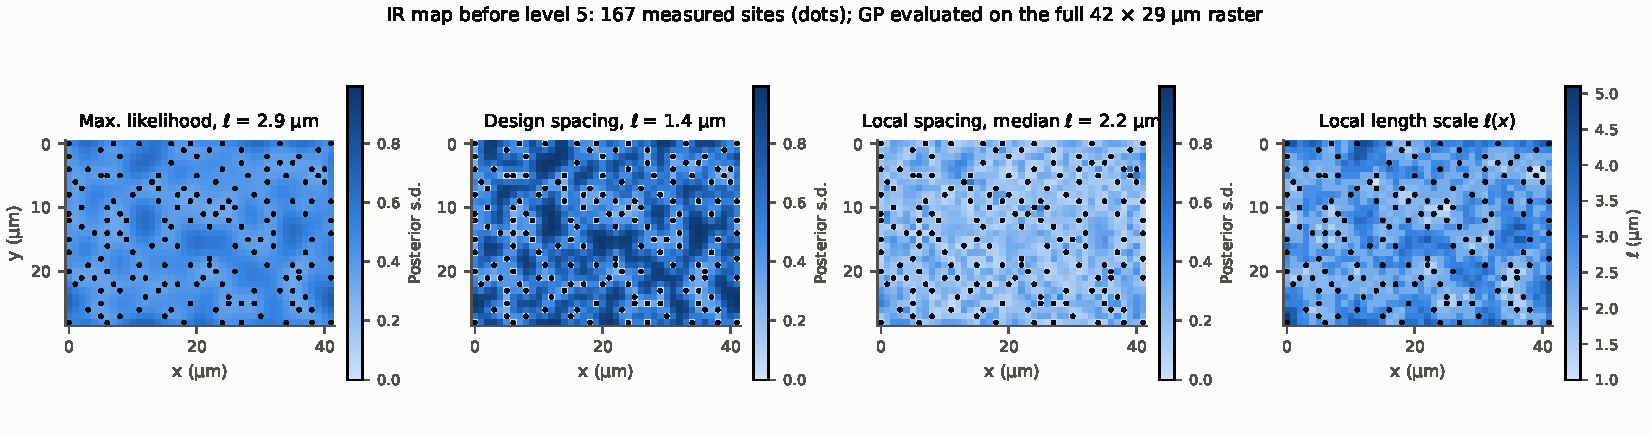
\includegraphics[width=\textwidth,height=0.44\textheight,keepaspectratio]{figures/figS1_gp_std}
\caption{Posterior standard deviation on the IR map before level 5 (first campaign of the record, local-spacing protocol; 167 measured sites, dots) under the three length-scale rules, evaluated on the full 42 \ensuremath{\times} 29 \ensuremath{\mu}m raster, and the local length scale of the third rule. Length scales are given in micrometres.}\label{fig:S1}
\end{figure}

\textbf{Checks.} Unit tests confirm that the weights reproduce the BoTorch posterior mean and variance for fixed hyperparameters, that the design rule follows the finest measured level, that the Gibbs kernel is positive semidefinite and reduces to the isotropic kernel for constant \(\ell\), and that the local length scale is long where measured sites are sparse.

\begin{center}\rule{0.5\linewidth}{0.5pt}\end{center}

\hypertarget{si-1.3-scores-of-the-natural-neighbour-protocol}{%
\subsection*{SI 1.3 Scores of the natural-neighbour protocol}\label{si-1.3-scores-of-the-natural-neighbour-protocol}}
\addcontentsline{toc}{subsection}{SI 1.3 Scores of the natural-neighbour protocol}

The interpolation score is one minus the probability of acceptance from a logistic regression, fitted by leave-one-out on the measured set (at most 120 sites) on the disagreement between natural neighbours in units of the acceptance metric and on the position. The interest score depends on the dataset. On the IR map it is the predicted maximum in the window, capped below the interest level, so that a site predicted to be of interest is never covered. On the two scattering datasets it is the probability of interest from a logistic regression on the predicted peak height above its baseline, the spread of that height over the five nearest measured sites and the distance to the nearest of them.

\hypertarget{si-2.-dataset-processing}{%
\section*{SI 2. Dataset processing}\label{si-2.-dataset-processing}}
\addcontentsline{toc}{section}{SI 2. Dataset processing}

\hypertarget{si-2.1-infrared-map}{%
\subsection*{SI 2.1 Infrared map}\label{si-2.1-infrared-map}}
\addcontentsline{toc}{subsection}{SI 2.1 Infrared map}

\textbf{Data.} The map covers 29 \ensuremath{\times} 42 pixels at a pitch of 1 \ensuremath{\mu}m, with 1738 channels between 650 and 4000 cm\ensuremath{^{-1}} in apparent absorbance. The claim window is 1500--1850 cm\ensuremath{^{-1}}. It holds the amide and ester bands, where scattering distortions are strongest next to the absorption bands.

\textbf{Scattering correction.} Particles of a few micrometres scatter infrared light resonantly. The result is broad oscillations and dispersive swings at band edges, superimposed on the absorbance. Each spectrum is corrected by extended multiplicative signal correction with a resonant Mie basis \cite{MartensStark1991,Kohler2005,Bassan2010,Solheim2019}. The measured apparent absorbance is modelled as a scaled chemical spectrum plus a scattering background:

\[ A(\nu) = b\,A_{\mathrm{c}}(\nu) + B(\nu) \]

The background is a combination of seven signed principal components of a family of scattering-only extinction curves in the van de Hulst approximation \cite{vandeHulst1957}. The family spans sphere radii of 2--8 \ensuremath{\mu}m, real refractive indices of 1.1--1.5 and imaginary indices peaking at 0.02--0.12, shaped by the current chemical estimate, with the dispersion obtained through the Kramers--Kronig relation. Absorption by the particles belongs to the chemical term and is left out of the basis. The fit has the following constraints:

\begin{itemize}
\tightlist
\item
  the background lies between zero and the measured spectrum;
\item
  b is at least 0.05;
\item
  the slope of the chemical spectrum is flat in 2100--2300 and 2390--2800 cm\ensuremath{^{-1}};
\item
  its level is pulled towards zero in 2390--2800 and 3850--4000 cm\ensuremath{^{-1}};
\item
  the background stays above the chord between these anchor windows across 2800--3850 cm\ensuremath{^{-1}}.
\end{itemize}

The chemical estimate is refined self-consistently. Each pixel starts from its own apparent absorbance, and after each of six iterations its estimate is replaced by its own corrected spectrum. No information passes between pixels, so the correction is a fixed transformation of each spectrum and can be applied to a site as soon as it is measured.

The corrected spectrum used throughout is the apparent absorbance minus the fitted background, clipped at zero; the scale b is not divided out. A site is of interest when any channel in the claim window reaches absorbance 0.1. That holds for 37 \% of the pixels.

\textbf{Sensitivity to the starting estimate.} The iteration converges to the same corrected spectrum for most pixels, whatever the starting estimate. Starting from the median spectrum of the map instead of each pixel\textquotesingle s own spectrum changes the corrected window by a median of 0.001. For about 5 \% of the pixels it changes it by more than 0.05, and 20 of 1218 pixels change their interest label. The guarantees of the main text concern the target as defined by the per-pixel correction. Any fixed per-spectrum transformation defines a valid target.

\textbf{Design.} The hierarchical Poisson-disk design is drawn on the physical rectangle, 41 \ensuremath{\times} 28 \ensuremath{\mu}m between the centres of the corner pixels. The radii run from 6.8 \ensuremath{\mu}m down to 0.85 \ensuremath{\mu}m in seven levels, each a factor \(\sqrt{2}\) below the previous one, with the four corners forced into the coarsest level. Sites are snapped to the nearest pixel, and the coarsest level is kept when two sites share a pixel. Of 1064 sites, 959 remain, with 23, 13, 37, 71, 142, 245 and 428 sites on levels 0--6. Distances for the interpolators are taken in micrometres, divided by 41 \ensuremath{\mu}m for numerical convenience. This rescaling is isotropic and leaves the geometry unchanged.

\hypertarget{si-2.2-nacl-microdiffraction-scan}{%
\subsection*{SI 2.2 NaCl microdiffraction scan}\label{si-2.2-nacl-microdiffraction-scan}}
\addcontentsline{toc}{subsection}{SI 2.2 NaCl microdiffraction scan}

The scan was recorded at beamline 7.3.3 of the Advanced Light Source and is used as deposited: azimuthally integrated profiles on a raster of 3249 sites with a stage step of 0.25 mm, each with 1000 bins between 0.589 and 38.94 nm\ensuremath{^{-1}} \cite{ALSNaCl}. Stage coordinates are rescaled to the unit square for the design and kept in millimetres for display. A hierarchical Poisson-disk design on the unit square, with radii from 0.2 to 0.025 over seven levels, is snapped to the nearest raster site; a raster site claimed by several design points keeps the coarsest level. The design holds 1071 sites, with 21, 19, 36, 65, 138, 271 and 521 sites on levels 0 to 6.

\textbf{The (200) line.} The (200) reflection of rock salt lies at \(q = 4\pi / a\) with \(a = 5.6402\) \AA{}, or 22.28 nm\ensuremath{^{-1}}. Its descriptors are taken in the window 22.28 \ensuremath{\pm} 0.40 nm\ensuremath{^{-1}}: the position of the tallest local maximum, refined by a parabola through the logarithms of intensity and \(q\), its height above a local baseline (the higher of the two flanking minima), and its full width at the level midway between baseline and peak.

\textbf{Noise and presence.} The noise in the window is estimated once from all design sites. Each profile is reduced to residuals from a straight baseline across the window. The 30 \% of profiles with the smallest largest residual are taken as off the ring, and the noise is 1.4826 times the median absolute deviation of their residuals: \(\sigma = 0.117\) in the units of the deposit. A line is present when its height above baseline exceeds \(5\sigma\); on that criterion 64 \% of the design sites hold the line, and these are the sites of interest. With this noise added twice, independently, to every measured profile, the second copy fails the width claim against the first at 1.1 \% \ensuremath{\pm} 0.3 \% of the 1071 design sites (20 repetitions).

\textbf{Width tolerance.} A prediction fails when it disagrees with the truth on the presence of the line, or when both show the line and their widths differ by more than 0.02 nm\ensuremath{^{-1}}. Sites without the line in truth and prediction pass. The same presence test is applied to the predicted profile, so a predicted line too weak to clear \(5\sigma\) counts as absent. The tolerance is set from the widths themselves, measured at all 3249 raster sites, without a model of what makes them vary. The width is read where the profile crosses half its height, interpolated between bins, so its precision is not tied to the bin width of 0.038 nm\ensuremath{^{-1}}. Over 40 copies of every profile with the noise above added, the width moved by a median of 0.0001 nm\ensuremath{^{-1}} and by at most 0.002 nm\ensuremath{^{-1}} at 90 \% of the sites holding the line. Across the sample the width runs from 0.057 to 0.141 nm\ensuremath{^{-1}} (5th to 95th percentile, median 0.098 nm\ensuremath{^{-1}}), and neighbouring raster sites, 0.25 mm apart, differ by a median of 0.018 nm\ensuremath{^{-1}}, rising to 0.022 nm\ensuremath{^{-1}} at the spacing of the finest design level (Table S2.1). The tolerance of 0.02 nm\ensuremath{^{-1}} lies ten times above the precision of the width and at the typical difference between neighbours, so a claim met at it says that the width varies little between a site and its surroundings; the variation is structure in the sample, and at this tolerance about half of all predictions from coarser levels fail whatever the model. Looser tolerances buy few measurements (Table S2.2).

{\renewcommand{\thetable}{S2.1}\small
\begin{longtable}[]{@{}
  >{\raggedright\arraybackslash}p{(\columnwidth - 10\tabcolsep) * \real{0.1667}}
  >{\raggedright\arraybackslash}p{(\columnwidth - 10\tabcolsep) * \real{0.1667}}
  >{\raggedright\arraybackslash}p{(\columnwidth - 10\tabcolsep) * \real{0.1667}}
  >{\raggedright\arraybackslash}p{(\columnwidth - 10\tabcolsep) * \real{0.1667}}
  >{\raggedright\arraybackslash}p{(\columnwidth - 10\tabcolsep) * \real{0.1667}}
  >{\raggedright\arraybackslash}p{(\columnwidth - 10\tabcolsep) * \real{0.1667}}@{}}
\caption{Absolute difference in the (200) width between pairs of raster sites holding the line, by distance; a site of the finest design level lies 0.35 mm from its nearest coarser site.}\label{tab:S2.1}\\

\toprule\noalign{}
\begin{minipage}[b]{\linewidth}\raggedright
distance (mm)
\end{minipage} & \begin{minipage}[b]{\linewidth}\raggedright
pairs
\end{minipage} & \begin{minipage}[b]{\linewidth}\raggedright
median (nm\ensuremath{^{-1}})
\end{minipage} & \begin{minipage}[b]{\linewidth}\raggedright
75th percentile (nm\ensuremath{^{-1}})
\end{minipage} & \begin{minipage}[b]{\linewidth}\raggedright
share above 0.02
\end{minipage} & \begin{minipage}[b]{\linewidth}\raggedright
share above 0.04
\end{minipage} \\
\midrule\noalign{}
\endhead
\bottomrule\noalign{}
\endlastfoot
0.25 & 3857 & 0.018 & 0.034 & 46 \% & 19 \% \\
0.26--0.50 & 7397 & 0.022 & 0.038 & 53 \% & 22 \% \\
0.50--1.00 & 37 759 & 0.022 & 0.039 & 55 \% & 24 \% \\
\end{longtable}
}

{\renewcommand{\thetable}{S2.2}\small
\begin{longtable}[]{@{}
  >{\raggedright\arraybackslash}p{(\columnwidth - 10\tabcolsep) * \real{0.1667}}
  >{\raggedright\arraybackslash}p{(\columnwidth - 10\tabcolsep) * \real{0.1667}}
  >{\raggedright\arraybackslash}p{(\columnwidth - 10\tabcolsep) * \real{0.1667}}
  >{\raggedright\arraybackslash}p{(\columnwidth - 10\tabcolsep) * \real{0.1667}}
  >{\raggedright\arraybackslash}p{(\columnwidth - 10\tabcolsep) * \real{0.1667}}
  >{\raggedright\arraybackslash}p{(\columnwidth - 10\tabcolsep) * \real{0.1667}}@{}}
\caption{Cost of the NaCl specification against tolerance and budget, matched-quantile rule with natural-neighbour prediction at confidence 0.80, 50 campaigns each. Shares are of the sites of levels 3 to 6.}\label{tab:S2.2}\\

\toprule\noalign{}
\begin{minipage}[b]{\linewidth}\raggedright
tolerance (nm\ensuremath{^{-1}})
\end{minipage} & \begin{minipage}[b]{\linewidth}\raggedright
budget
\end{minipage} & \begin{minipage}[b]{\linewidth}\raggedright
measured
\end{minipage} & \begin{minipage}[b]{\linewidth}\raggedright
mean share skipped in error
\end{minipage} & \begin{minipage}[b]{\linewidth}\raggedright
level checks over budget
\end{minipage} & \begin{minipage}[b]{\linewidth}\raggedright
campaigns over on some level
\end{minipage} \\
\midrule\noalign{}
\endhead
\bottomrule\noalign{}
\endlastfoot
0.02 & 0.10 & 799 \ensuremath{\pm} 67 & 5.7 \% & 12.5 \% & 38 \% \\
0.02 & 0.20 & 619 \ensuremath{\pm} 62 & 14.4 \% & 10.5 \% & 38 \% \\
0.03 & 0.10 & 764 \ensuremath{\pm} 85 & 6.0 \% & 10.0 \% & 32 \% \\
0.03 & 0.20 & 570 \ensuremath{\pm} 56 & 14.5 \% & 9.5 \% & 30 \% \\
0.04 & 0.10 & 733 \ensuremath{\pm} 84 & 5.9 \% & 13.5 \% & 38 \% \\
0.04 & 0.20 & 516 \ensuremath{\pm} 61 & 15.1 \% & 11.5 \% & 38 \% \\
0.05 & 0.10 & 694 \ensuremath{\pm} 94 & 6.1 \% & 12.5 \% & 38 \% \\
0.05 & 0.20 & 478 \ensuremath{\pm} 54 & 15.1 \% & 10.0 \% & 32 \% \\
\end{longtable}
}

The interest claim and the calibration draws set a floor of about 240 measured sites at every tolerance, and loosening the tolerance from 0.02 to 0.05 nm\ensuremath{^{-1}} saved 105 to 141 measurements. Level checks over budget stayed near the picked failure probabilities, about 12 \% on average.

\hypertarget{si-2.3-synthetic-small-angle-scattering-map}{%
\subsection*{SI 2.3 Synthetic small-angle scattering map}\label{si-2.3-synthetic-small-angle-scattering-map}}
\addcontentsline{toc}{subsection}{SI 2.3 Synthetic small-angle scattering map}

\textbf{Forward model.} A composition \((x, y)\), with \(x\) the oil and \(y\) the surfactant weight fraction and \(x + y \le 1\), maps to a noiseless scattering curve on 240 logarithmically spaced points between 0.005 and 0.32 \AA{}\ensuremath{^{-1}}. Four phases are separated by straight boundaries in composition: a micellar phase (L1), modelled as polydisperse spheres whose radius swells with solubilised oil, with a Percus--Yevick hard-sphere structure factor; an ordered cubic phase (I1) with face-centred cubic Bragg peaks; a hexagonal phase (H1) with Bragg peaks of a two-dimensional hexagonal lattice and a cylinder form factor; and an oil-rich emulsion, in which excess oil adds Porod scattering. Sigmoids of fixed width smooth every transition, so the curves vary continuously with composition while the peak positions and widths change quickly near the boundaries. The model is carried over from an earlier study and is deposited with the data.

\textbf{Parameters.} Table S2.3 lists every parameter of the forward model; the curves carry no noise.

{\renewcommand{\thetable}{S2.3}\small
\begin{longtable}[]{@{}
  >{\raggedright\arraybackslash}p{(\columnwidth - 4\tabcolsep) * \real{0.3333}}
  >{\raggedright\arraybackslash}p{(\columnwidth - 4\tabcolsep) * \real{0.3333}}
  >{\raggedright\arraybackslash}p{(\columnwidth - 4\tabcolsep) * \real{0.3333}}@{}}
\caption{Parameters of the synthetic forward model (compositions in weight fractions, lengths in \AA{}, \(q\) in \AA{}\ensuremath{^{-1}}).}\label{tab:S2.3}\\

\toprule\noalign{}
\begin{minipage}[b]{\linewidth}\raggedright
Group
\end{minipage} & \begin{minipage}[b]{\linewidth}\raggedright
Parameter
\end{minipage} & \begin{minipage}[b]{\linewidth}\raggedright
Value
\end{minipage} \\
\midrule\noalign{}
\endhead
\bottomrule\noalign{}
\endlastfoot
Phase boundaries & emulsion: \(x = 0.15 + 0.55\,y\); order--disorder: \(y = 0.42 + 0.50\,x\); cubic--hexagonal: \(y = 0.72 + 0.30\,x\) & sigmoid widths 0.012 \\
Micelles (L1) & dry radius \(R_0\), cap on swollen radius, swelling strength & 60, 95, 1.2 \\
& polydispersity (Gaussian, relative), quadrature points & 0.08, 15 \\
& hard-sphere radius / micelle radius; volume fraction per surfactant fraction, range & 1.25; 0.9, 0.05--0.45 \\
Ordered phases & FCC (111) position at \((0, 0.5)\); resolution-limited width; extra width near the transition & 0.045, 0.0016, 0.004 \\
& FCC peak ratios and amplitudes & \(\sqrt{3,4,8,11,12}/\sqrt{3}\); 30, 9, 5, 2.5, 1.5 \\
& hexagonal peak ratios and amplitudes; \(q^\ast\) relative to FCC & \(\sqrt{1,3,4,7}\); 40, 8, 5, 2; 1.25 \\
Emulsion and background & Porod amplitude per 0.1 excess oil; flat background & \(4 \times 10^{-8}\); \(5 \times 10^{-5}\) \\
Intensity & amplitude per surfactant fraction; floor & 2.0; 0.02 \\
\end{longtable}
}

\textbf{Design.} A hierarchical Poisson-disk design on the unit square with nine levels, with the corners forced into the coarsest level, is restricted to the triangle \(x + y \le 1\), which leaves 2118 sites. The natural-neighbour interpolant adds mirror images of the measured sites across \(x = 0\), \(y = 0\) and \(x + y = 1\), and across the origin, each carrying the spectrum of its preimage (SI 1.1).

\textbf{Descriptors and claims.} The dominant peak is the tallest interior local maximum, its position refined below the grid spacing by a parabola in logarithmic coordinates; its width and height above baseline are measured as for the NaCl line. A site is of interest when its dominant peak rises above its local baseline by at least five times that baseline, which holds for most ordered compositions and for part of the micellar phase. A prediction fails when it disagrees on the presence of a dominant peak, or misses its position by more than 0.005 \AA{}\ensuremath{^{-1}} or its width by more than 0.001 \AA{}\ensuremath{^{-1}}. Sites without a peak in truth and prediction pass.

\hypertarget{si-3.-full-tables-per-dataset-level-and-protocol}{%
\section*{SI 3. Full tables per dataset, level and protocol}\label{si-3.-full-tables-per-dataset-level-and-protocol}}
\addcontentsline{toc}{section}{SI 3. Full tables per dataset, level and protocol}

\emph{Per-level tables for every configuration are in the run record (SI 5); the tables below summarise them. All entries: mean \ensuremath{\pm} s.d. over 250 campaigns, 20 for the Gaussian-process protocols of the synthetic map.}

{\renewcommand{\thetable}{S3.1}\small
\begin{longtable}[]{@{}
  >{\raggedright\arraybackslash}p{(\columnwidth - 8\tabcolsep) * \real{0.2000}}
  >{\raggedright\arraybackslash}p{(\columnwidth - 8\tabcolsep) * \real{0.2000}}
  >{\raggedright\arraybackslash}p{(\columnwidth - 8\tabcolsep) * \real{0.2000}}
  >{\raggedright\arraybackslash}p{(\columnwidth - 8\tabcolsep) * \real{0.2000}}
  >{\raggedright\arraybackslash}p{(\columnwidth - 8\tabcolsep) * \real{0.2000}}@{}}
\caption{Sites measured for each form of guarantee for the same stated bound on the shared skip-error rate: \(R_E \le 0.10\) at confidence 0.75 for the IR map and \(R_E \le 0.20\) at confidence 0.80 for the NaCl scan. The synthetic map carries one claim, so its three forms coincide; it is given once. Same data as Fig. S3, upper row.}\label{tab:S3.1}\\

\toprule\noalign{}
\begin{minipage}[b]{\linewidth}\raggedright
Dataset
\end{minipage} & \begin{minipage}[b]{\linewidth}\raggedright
Design sites
\end{minipage} & \begin{minipage}[b]{\linewidth}\raggedright
Per-claim budgets
\end{minipage} & \begin{minipage}[b]{\linewidth}\raggedright
Matched-quantile rule
\end{minipage} & \begin{minipage}[b]{\linewidth}\raggedright
Priority rule
\end{minipage} \\
\midrule\noalign{}
\endhead
\bottomrule\noalign{}
\endlastfoot
IR map & 959 & 262 \ensuremath{\pm} 28 & 295 \ensuremath{\pm} 53 & 327 \ensuremath{\pm} 80 \\
NaCl scan & 1071 & 719 \ensuremath{\pm} 60 & 614 \ensuremath{\pm} 56 & 678 \ensuremath{\pm} 39 \\
Synthetic map (\(R_E \le 0.10\) at 0.80, one claim) & 2118 & 932 \ensuremath{\pm} 223 & 932 \ensuremath{\pm} 223 & 932 \ensuremath{\pm} 223 \\
\end{longtable}
}

{\renewcommand{\thetable}{S3.2}\small
\begin{longtable}[]{@{}
  >{\raggedright\arraybackslash}p{(\columnwidth - 10\tabcolsep) * \real{0.1667}}
  >{\raggedright\arraybackslash}p{(\columnwidth - 10\tabcolsep) * \real{0.1667}}
  >{\raggedright\arraybackslash}p{(\columnwidth - 10\tabcolsep) * \real{0.1667}}
  >{\raggedright\arraybackslash}p{(\columnwidth - 10\tabcolsep) * \real{0.1667}}
  >{\raggedright\arraybackslash}p{(\columnwidth - 10\tabcolsep) * \real{0.1667}}
  >{\raggedright\arraybackslash}p{(\columnwidth - 10\tabcolsep) * \real{0.1667}}@{}}
\caption{Sites measured for each interpolation protocol under the matched-quantile rule, at the same nominal guarantees. Same data as Fig. 6. The tight IR tolerance is \ensuremath{\pm}(10 \% + 0.01) absorbance with interest at 0.02; the last row uses the interpolation claim alone.}\label{tab:S3.2}\\

\toprule\noalign{}
\begin{minipage}[b]{\linewidth}\raggedright
Dataset
\end{minipage} & \begin{minipage}[b]{\linewidth}\raggedright
Design sites
\end{minipage} & \begin{minipage}[b]{\linewidth}\raggedright
Natural neighbour
\end{minipage} & \begin{minipage}[b]{\linewidth}\raggedright
GP, max. likelihood
\end{minipage} & \begin{minipage}[b]{\linewidth}\raggedright
GP, design spacing
\end{minipage} & \begin{minipage}[b]{\linewidth}\raggedright
GP, local spacing
\end{minipage} \\
\midrule\noalign{}
\endhead
\bottomrule\noalign{}
\endlastfoot
IR map & 959 & 295 \ensuremath{\pm} 53 & 273 \ensuremath{\pm} 31 & 281 \ensuremath{\pm} 34 & 291 \ensuremath{\pm} 41 \\
IR map, tight & 959 & 621 \ensuremath{\pm} 70 & 747 \ensuremath{\pm} 56 & 753 \ensuremath{\pm} 52 & 799 \ensuremath{\pm} 40 \\
IR map, tight, interpolation only & 959 & 604 \ensuremath{\pm} 65 & 792 \ensuremath{\pm} 58 & 797 \ensuremath{\pm} 56 & 854 \ensuremath{\pm} 35 \\
NaCl scan & 1071 & 614 \ensuremath{\pm} 56 & 745 \ensuremath{\pm} 72 & 760 \ensuremath{\pm} 70 & 777 \ensuremath{\pm} 60 \\
Synthetic map (GP: 20 campaigns) & 2118 & 932 \ensuremath{\pm} 223 & 1974 \ensuremath{\pm} 55 & 1946 \ensuremath{\pm} 50 & 2027 \ensuremath{\pm} 39 \\
\end{longtable}
}

{\renewcommand{\thetable}{S3.3}\small
\begin{longtable}[]{@{}llll@{}}
\caption{Sites measured with random scores for every claim, against informed scores (Fig. 6).}\label{tab:S3.3}\\

\toprule\noalign{}
Dataset & Form & Informed scores & Random scores \\
\midrule\noalign{}
\endhead
\bottomrule\noalign{}
\endlastfoot
IR map & Per-claim budgets & 262 \ensuremath{\pm} 28 & 335 \ensuremath{\pm} 84 \\
IR map & Matched-quantile rule & 295 \ensuremath{\pm} 53 & 716 \ensuremath{\pm} 71 \\
IR map & Priority rule & 327 \ensuremath{\pm} 80 & 817 \ensuremath{\pm} 49 \\
IR map, tight & Matched-quantile rule & 621 \ensuremath{\pm} 70 & 871 \ensuremath{\pm} 31 \\
NaCl scan & Per-claim budgets & 719 \ensuremath{\pm} 60 & 928 \ensuremath{\pm} 45 \\
NaCl scan & Matched-quantile rule & 614 \ensuremath{\pm} 56 & 861 \ensuremath{\pm} 50 \\
NaCl scan & Priority rule & 678 \ensuremath{\pm} 39 & 874 \ensuremath{\pm} 49 \\
Synthetic map & One claim (all forms) & 932 \ensuremath{\pm} 223 & 1578 \ensuremath{\pm} 248 \\
\end{longtable}
}

\begin{figure}[tbp]\renewcommand{\thefigure}{S3}
\centering
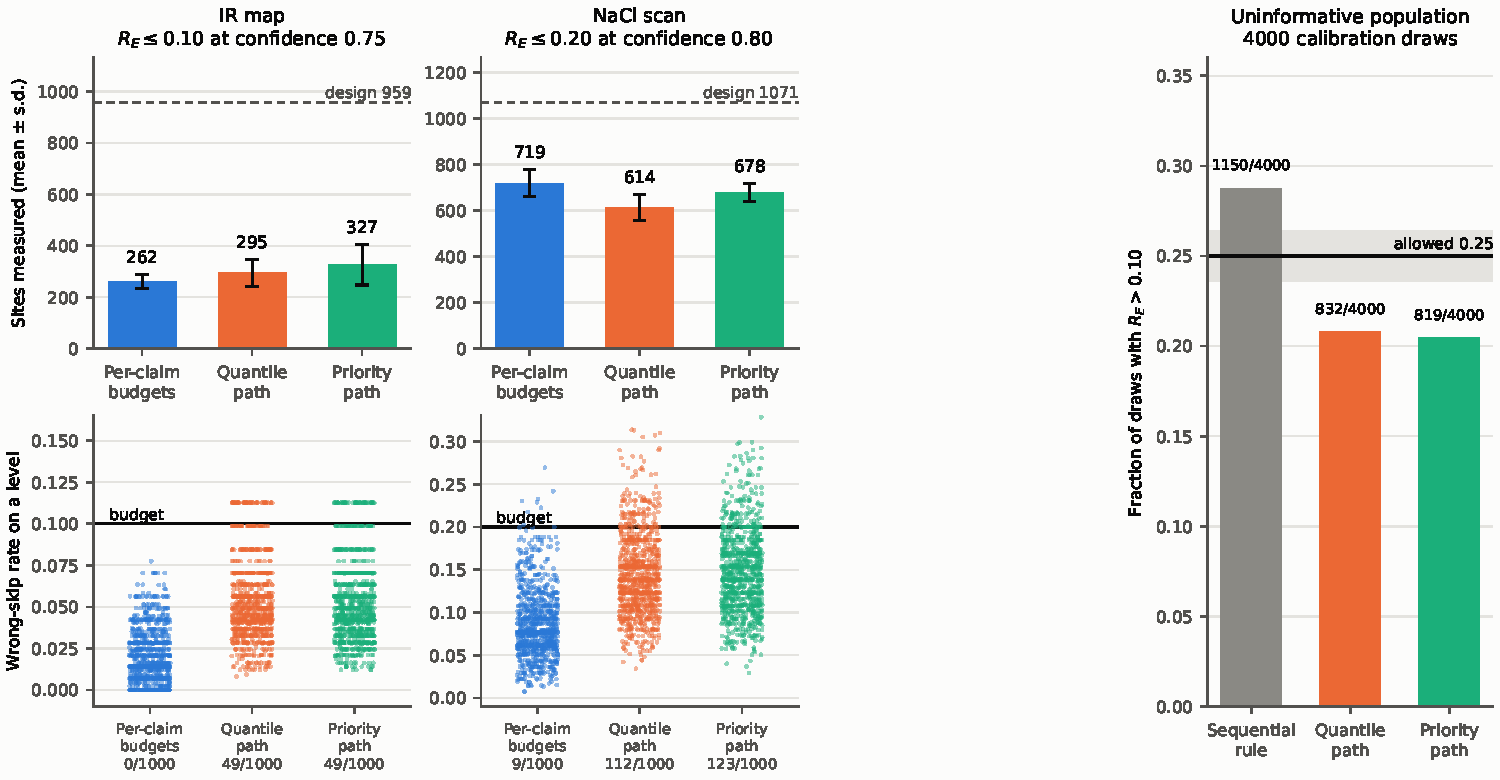
\includegraphics[width=\textwidth,height=0.44\textheight,keepaspectratio]{figures/fig3_forms}
\caption{Forms of guarantee, 250 campaigns per configuration. Upper row: sites measured per form, mean \ensuremath{\pm} s.d., with the design size dashed. Lower row: realised skip-error rate on every guaranteed level of every campaign, with the budget as a solid line; tick labels give the number of exceedances. Right: fraction of 4000 calibration draws in which \(R_E\) exceeded 0.10 on a population with uninformative scores, for the sequential rule and the two single-budget paths; the band marks \ensuremath{\pm}2 Monte Carlo standard errors around the allowed 0.25.}\label{fig:S3}
\end{figure}

\hypertarget{forms-of-guarantee-and-random-scores-compared}{%
\subsection*{Forms of guarantee and random scores compared}\label{forms-of-guarantee-and-random-scores-compared}}
\addcontentsline{toc}{subsection}{Forms of guarantee and random scores compared}

Every form of Table S4.3 kept its guarantee on the two maps with two claims at one nominal statement on the shared event, \(R_E \le 0.10\) at confidence 0.75 for IR and \(R_E \le 0.20\) at 0.80 for NaCl (Fig. S3; Table S3.1); with the one claim of the synthetic map the forms coincide. The shared rate exceeded its budget in 0, 49 and 49 of 1000 level checks for the per-claim form, the matched-quantile rule and the priority rule on IR, and in 9, 112 and 123 of 1000 on NaCl. No form was the least expensive on all three maps: the per-claim form measured 262 \ensuremath{\pm} 28 of 959 sites on IR against 295 \ensuremath{\pm} 53 for the matched-quantile rule, and the matched-quantile rule 614 \ensuremath{\pm} 56 of 1071 on NaCl against 678 to 719. The sequential rule of an earlier analysis of the IR map, which sets the interpolation threshold on the calibration sites left uncovered by the interest threshold, exceeded \(R_E = 0.10\) in 28.8 \% of 4000 draws; the priority rule, which fixes the same preference in advance, did so in 20.5 \%, at a picked failure probability of 20.6 \%.

With random scores, an independent uniform weight per site and claim, the shared rate exceeded its budget in 168 of 1000 level checks on IR, 194 of 1000 on IR at the tight tolerance, 127 of 1000 on NaCl and 149 of 1500 on the synthetic map, at nominal failure probabilities of 0.25, 0.25, 0.20 and 0.20 (Table S3.3).

\hypertarget{si-4.-software-adding-a-form-of-guarantee}{%
\section*{SI 4. Software: adding a form of guarantee}\label{si-4.-software-adding-a-form-of-guarantee}}
\addcontentsline{toc}{section}{SI 4. Software: adding a form of guarantee}

\hypertarget{si-4.1-interface-for-a-form-of-guarantee}{%
\subsection*{SI 4.1 Interface for a form of guarantee}\label{si-4.1-interface-for-a-form-of-guarantee}}
\addcontentsline{toc}{subsection}{SI 4.1 Interface for a form of guarantee}

A form of guarantee is a budget policy in the \texttt{accountable} package. It implements \texttt{decide(LevelData)\ -\textgreater{}\ PolicyDecision} and registers a name with \texttt{@register("name")}. The forms in the main text are the policies \texttt{separate} (per-claim budgets), \texttt{nested\_path} (matched-quantile rule) and \texttt{priority\_path} (priority rule); \texttt{ltt\_conditional} gives the conditional rate of Appendix C.

A policy keeps three conditions.

\begin{enumerate}
\def\labelenumi{\arabic{enumi}.}
\tightlist
\item
  \textbf{Inputs.} It uses the frozen scores of every site of the level, the indices of the calibration sites and the bad labels of those sites only. Scores are frozen before the draw and are not refitted by the policy.
\item
  \textbf{Fixed family.} Every family of thresholds it searches (a path, a grid, a split of the budget) is built from scores, settings or earlier levels, and from no calibration label of the current level.
\item
  \textbf{Stated guarantee.} It returns its guarantees as \texttt{Guarantee(event,\ budget,\ confidence)}, with \texttt{event} equal to \texttt{R\_E} or \texttt{R\_\textless{}claim\textgreater{}}, or an empty list. Campaign records show an empty list as "no guarantee".
\end{enumerate}

Condition 2 carries the proof of Appendix B. The sequential rule of Section 5.1 violates it.

The campaign loop enforces the order of operations of Section 3.1 structurally: a score receives only the measured set (\texttt{MeasuredSet}) when it is fitted and is frozen with \texttt{bind\_level} before the draw; the calibration indices come from a generator that nothing else uses; and a policy receives the labels of the calibration sites only. A policy or score written against these interfaces cannot see the labels of the level it is deciding before the draw.

\hypertarget{si-4.2-acceptance-check}{%
\subsection*{SI 4.2 Acceptance check}\label{si-4.2-acceptance-check}}
\addcontentsline{toc}{subsection}{SI 4.2 Acceptance check}

Before a policy carries a claim, each guarantee it states is checked by Monte Carlo on fixed finite populations (\texttt{accountable.validate.check\_coverage}). The population is fixed, so the calibration draw is the only randomness. For each stated guarantee, the check counts the draws in which the population rate exceeds the budget and compares that frequency with \(1 - \text{confidence}\), allowing three Monte Carlo standard errors. Scores are drawn uniform on \([0, 1]\); labels are independent of the scores (uninformative, the hard case) or have a bad probability rising linearly with the score at the same mean (informative).

{\renewcommand{\thetable}{S4.1}\small
\begin{longtable}[]{@{}
  >{\raggedright\arraybackslash}p{(\columnwidth - 8\tabcolsep) * \real{0.2000}}
  >{\raggedright\arraybackslash}p{(\columnwidth - 8\tabcolsep) * \real{0.2000}}
  >{\raggedright\arraybackslash}p{(\columnwidth - 8\tabcolsep) * \real{0.2000}}
  >{\raggedright\arraybackslash}p{(\columnwidth - 8\tabcolsep) * \real{0.2000}}
  >{\raggedright\arraybackslash}p{(\columnwidth - 8\tabcolsep) * \real{0.2000}}@{}}
\caption{Acceptance check on a population of 271 sites, \(m = 40\), 2000 draws; interest and interpolation labels at mean rates 0.30 and 0.35. Entries are the fraction of draws in which the stated rate exceeded its budget.}\label{tab:S4.1}\\

\toprule\noalign{}
\begin{minipage}[b]{\linewidth}\raggedright
Policy
\end{minipage} & \begin{minipage}[b]{\linewidth}\raggedright
Stated guarantee
\end{minipage} & \begin{minipage}[b]{\linewidth}\raggedright
Allowed
\end{minipage} & \begin{minipage}[b]{\linewidth}\raggedright
Uninformative
\end{minipage} & \begin{minipage}[b]{\linewidth}\raggedright
Informative
\end{minipage} \\
\midrule\noalign{}
\endhead
\bottomrule\noalign{}
\endlastfoot
Per-claim budgets & \(R_{\mathrm{interest}} \le 0.10\) & 0.10 & 0.039 & 0.047 \\
& \(R_{\mathrm{interp}} \le 0.10\) & 0.10 & 0.036 & 0.027 \\
& \(R_E \le 0.20\) & 0.20 & 0.010 & 0.004 \\
Matched-quantile rule & \(R_E \le 0.10\) & 0.10 & 0.047 & 0.045 \\
Priority rule, interest first & \(R_E \le 0.10\) & 0.10 & 0.039 & 0.047 \\
Priority rule, interpolation first & \(R_E \le 0.10\) & 0.10 & 0.036 & 0.027 \\
Plug-in rule (counterexample) & \(R_{\mathrm{interp}} \le 0.10\) & 0.10 & 0.554 & 0.515 \\
\end{longtable}
}

The plug-in rule takes the largest threshold whose empirical calibration rate stays within the budget, with no order-statistic correction, and states a guarantee at confidence 0.90. The check rejects it. Passing the check is evidence for a policy; the finite-sample argument still has to be written down, as in Appendix B.

\hypertarget{si-4.3-worked-example-the-priority-rule}{%
\subsection*{SI 4.3 Worked example: the priority rule}\label{si-4.3-worked-example-the-priority-rule}}
\addcontentsline{toc}{subsection}{SI 4.3 Worked example: the priority rule}

The priority rule subclasses the matched-quantile rule and replaces only the entry times: claim \(i\) in the order sweeps its own score quantiles over \(\lambda \in (i, i + 1]\) (Appendix B.2). The order is a setting, so the family is fixed before the draw and Proposition B.2 applies without change. The implementation is about thirty lines. Unit tests check that the priority rule with one claim gives the same covers as the single-claim rule, and that both orders pass the acceptance check.

\hypertarget{si-4.4-software-tests-and-reproduction}{%
\subsection*{SI 4.4 Software, tests and reproduction}\label{si-4.4-software-tests-and-reproduction}}
\addcontentsline{toc}{subsection}{SI 4.4 Software, tests and reproduction}

\textbf{Functionality.} The workflow is a Python package with four parts: (i) the campaign loop, which runs the five steps of Section 3.1 on any dataset that supplies design sites, levels and an oracle for the measurement at a site; (ii) the forms of guarantee of Section 3.4 as budget policies, with exact hypergeometric and binomial tails; (iii) predictors and scores, natural-neighbour interpolation with mirror images at boundaries and Gaussian-process interpolation under three length-scale rules; (iv) the record, which writes every site\textquotesingle s level, scores, action and reason and every level\textquotesingle s calibration draw, thresholds and picked failure probability, together with the random state, so that each campaign can be replayed and every bound recomputed.

\textbf{Tests.} The test suite checks the geometry of the natural-neighbour weights, the Gaussian-process engine, the acceptance check of Table S4.1 for every policy, the coverage of every stated guarantee by Monte Carlo on fixed populations (including that the sequential rule exceeds its nominal rate), and that recorded campaigns replay to identical decisions. The implementation refuses a binomial allowance \(k\) larger than the hypergeometric one; no such case arose in this study.

\textbf{Reproduction.} Each figure and table of the main text and of this supplement is produced by a script that reads only the run record; the record is produced by re-running the configurations of Table S4.2 with random states 0 to 249. A campaign takes 3 to 12 s on one core.

{\renewcommand{\thetable}{S4.2}\small
\begin{longtable}[]{@{}
  >{\raggedright\arraybackslash}p{(\columnwidth - 2\tabcolsep) * \real{0.5000}}
  >{\raggedright\arraybackslash}p{(\columnwidth - 2\tabcolsep) * \real{0.5000}}@{}}
\caption{Configuration names in the record and the protocols of the main text.}\label{tab:S4.2}\\

\toprule\noalign{}
\begin{minipage}[b]{\linewidth}\raggedright
Name element
\end{minipage} & \begin{minipage}[b]{\linewidth}\raggedright
Meaning
\end{minipage} \\
\midrule\noalign{}
\endhead
\bottomrule\noalign{}
\endlastfoot
\texttt{ir}, \texttt{ir\_\allowbreak{}tight}, \texttt{nacl\_\allowbreak{}fwhm}, \texttt{syn\_\allowbreak{}env}, \texttt{syn\_\allowbreak{}peak\_\allowbreak{}2cert} & IR map at the original and the tight tolerance; NaCl scan, width claim; synthetic map, full-profile claim alone (main text); synthetic map, peak and interest claims (variant of SI 6.2) \\
\texttt{separate}, \texttt{nested}, \texttt{priority} & per-claim budgets, matched-quantile rule, priority rule (Section 3.4) \\
\texttt{watson}, \texttt{sibson} & natural-neighbour (Sibson) interpolation with the logistic score; \texttt{watson} names the construction of the weights \\
\texttt{gp\_\allowbreak{}mle}, \texttt{gp\_\allowbreak{}design}, \texttt{gp\_\allowbreak{}nonstationary} & Gaussian-process interpolation, length scale by maximum likelihood, by design spacing, by local spacing \\
\texttt{random} & random scores for every claim \\
\texttt{legacy\_\allowbreak{}sequential} & the sequential rule of the original IR analysis (Appendix B.3) \\
\end{longtable}
}

\hypertarget{si-4.5-the-forms-of-guarantee}{%
\subsection*{SI 4.5 The forms of guarantee}\label{si-4.5-the-forms-of-guarantee}}
\addcontentsline{toc}{subsection}{SI 4.5 The forms of guarantee}

Section 3.4 of the main text defines the shared skip-error event \(E\) and its rate \(R_E\) over a level. The forms below spend the budget on it in different ways; every form uses the same frozen scores and the same calibration draw.

\textbf{Per-claim budgets.} Each claim is calibrated on its own, with budget \(\varepsilon_j\) and failure probability \(\delta_j\), on one shared draw. A skip error fails at least one claim, so \(R_E \le R_a + R_b\), and the Bonferroni inequality gives

\[
P\big(R_E \le \varepsilon_a + \varepsilon_b\big) \ge 1 - \delta_a - \delta_b
\]

alongside a separate guarantee for each claim. The split leaves each claim a smaller budget at a higher confidence. Once \(\varepsilon_j\) falls below \(\varepsilon_{\min}\), no threshold exists and the level is measured in full.

\textbf{One budget along a path.} A single budget spends all of \(\varepsilon\) and \(\delta\) on \(R_E\). Two thresholds cannot be read off one draw by an order statistic, and Learn-then-Test supplies the remedy: search a family of thresholds fixed before any label is seen \cite{Angelopoulos2025}. Here the family is a path \(\lambda \mapsto (\tau_a(\lambda), \tau_b(\lambda))\), built from the frozen scores alone, along which both thresholds rise. The skip-error sets along such a path are nested, \(R_E(\lambda)\) grows with \(\lambda\), and the rule of Section 3.3 of the main text applies with \(\lambda\) in place of the threshold (Appendix B). Two paths are used. The matched-quantile rule moves both thresholds through matching quantiles of their scores on the level. The priority rule admits the claims in a set order: the first claim sweeps its quantiles before the second moves. A preference between the claims thereby enters the decision with the guarantee intact.

\textbf{Further forms.} Any rule built from scores frozen before the draw, a uniform calibration draw and a family of thresholds fixed before the labels are known inherits a finite-sample guarantee, including a bound on a conditional rate (Appendix C). A label-conditional statement protects the sites of interest: given their number, the calibration sites of interest are a uniform draw from those of the level, and the rule of Section 3.3 of the main text, with the worst case over their unknown total, limits the share skipped under the no-interest claim \cite{Vovk2005,Sadinle2019,Tong2018}; a cover so restricted keeps every bound on a rate counted over the level, provided the budget it frees is not spent again on the same draw (Appendix B.3). The statement bounds a share of the sites of interest, not where the lost ones lie, and holds per level; with the shared bound on the same draw, both hold with probability at least \(1 - \delta_L - \delta_Z\), where \(\delta_Z\) is the failure probability of the conditional statement. Table S4.3 summarises the forms; Section SI 4.2 gives the Monte Carlo acceptance check every form passes.

{\renewcommand{\thetable}{S4.3}\small
\begin{longtable}[]{@{}
  >{\raggedright\arraybackslash}p{(\columnwidth - 8\tabcolsep) * \real{0.2000}}
  >{\raggedright\arraybackslash}p{(\columnwidth - 8\tabcolsep) * \real{0.2000}}
  >{\raggedright\arraybackslash}p{(\columnwidth - 8\tabcolsep) * \real{0.2000}}
  >{\raggedright\arraybackslash}p{(\columnwidth - 8\tabcolsep) * \real{0.2000}}
  >{\raggedright\arraybackslash}p{(\columnwidth - 8\tabcolsep) * \real{0.2000}}@{}}
\caption{Forms of guarantee on the skip-error event of one level. Every form uses the same frozen scores and the same calibration draw.}\label{tab:S4.3}\\

\toprule\noalign{}
\begin{minipage}[b]{\linewidth}\raggedright
Form
\end{minipage} & \begin{minipage}[b]{\linewidth}\raggedright
Guarantee, with probability at least the stated confidence
\end{minipage} & \begin{minipage}[b]{\linewidth}\raggedright
Budget
\end{minipage} & \begin{minipage}[b]{\linewidth}\raggedright
Given up
\end{minipage} & \begin{minipage}[b]{\linewidth}\raggedright
Suited to
\end{minipage} \\
\midrule\noalign{}
\endhead
\bottomrule\noalign{}
\endlastfoot
Per-claim budgets & \(R_a \le \varepsilon_a\) and \(R_b \le \varepsilon_b\); hence \(R_E \le \varepsilon_a + \varepsilon_b\) at \(1 - \delta_a - \delta_b\) & Split between the claims & Budget per claim; no threshold once \(\varepsilon_j < \varepsilon_{\min}\) & Reporting how often each reason for skipping fails \\
Matched-quantile rule & \(R_E \le \varepsilon\) at \(1 - \delta\) & Whole budget on \(R_E\) & Guarantee per claim; path shape set in advance & Bounding how often any skip fails \\
Priority rule & \(R_E \le \varepsilon\) at \(1 - \delta\) & Whole budget on \(R_E\), spent on the claims in order & Guarantee per claim; a later claim may receive no budget & A set preference between the claims \\
Conditional rate (Appendix C) & Failure rate among sites skipped by one claim \(\le \alpha\) at \(1 - \delta\) & One claim & Coverage at small \(m\): at \(m = 40\) it guarantees nothing or more than half a level & Large calibration samples \\
\end{longtable}
}

\hypertarget{si-5.-the-run-record}{%
\section*{SI 5. The run record}\label{si-5.-the-run-record}}
\addcontentsline{toc}{section}{SI 5. The run record}

From round 3 the synthetic map carries the interpolation claim alone on the full profile (rtol = atol = 0.005) at a budget of 0.10 and confidence 0.80; with one claim the three forms of guarantee coincide, so one configuration stands for them. The two-claim configurations used before are kept in the record and in the archive of earlier results. Every configuration of Section 5 was run as 250 independent campaigns, random states 0 to 249, except the four Gaussian-process configurations of the synthetic map, run as 20 (random states 0 to 19) for their cost of one to three minutes each, and the NaCl process scored by its own failure probability, run as 50; a random state fixes the calibration draws of a campaign and, for random scores, the score stream. 34 configurations give 7380 campaigns; the comparisons of SI 5.3 add 250 campaigns each of three rules on three maps. Each campaign is logged in full: its configuration, every per-level record (thresholds, the allowed number of calibration failures under both the binomial and the exact finite-population tail, the stated guarantees, calibration counts, level and remainder rates, map bound), the decision and reason for every design site, the interest and interpolation labels of every site and the frozen score of each claim. The record also holds the code version, the package versions and the wall time of each campaign. For the maximum-likelihood Gaussian-process configurations, the end-of-level and final-map labels, which need a refit on the full measured set and change no decision, were not computed. The record lives in the repository under results/record (one directory per configuration: a compressed line-per-campaign log and a compressed array file), with a manifest, the summary below and the audit table.

{\renewcommand{\thetable}{S5.1}\small
\begin{longtable}[]{@{}
  >{\raggedright\arraybackslash}p{(\columnwidth - 16\tabcolsep) * \real{0.1111}}
  >{\raggedright\arraybackslash}p{(\columnwidth - 16\tabcolsep) * \real{0.1111}}
  >{\raggedright\arraybackslash}p{(\columnwidth - 16\tabcolsep) * \real{0.1111}}
  >{\raggedright\arraybackslash}p{(\columnwidth - 16\tabcolsep) * \real{0.1111}}
  >{\raggedright\arraybackslash}p{(\columnwidth - 16\tabcolsep) * \real{0.1111}}
  >{\raggedright\arraybackslash}p{(\columnwidth - 16\tabcolsep) * \real{0.1111}}
  >{\raggedright\arraybackslash}p{(\columnwidth - 16\tabcolsep) * \real{0.1111}}
  >{\raggedright\arraybackslash}p{(\columnwidth - 16\tabcolsep) * \real{0.1111}}
  >{\raggedright\arraybackslash}p{(\columnwidth - 16\tabcolsep) * \real{0.1111}}@{}}
\caption{Exceedances of every stated rate over all guaranteed levels of all campaigns. "Allowed failure" is one minus the stated confidence; the interval is a 95 \% Clopper--Pearson interval on the exceedance frequency (indicative, since levels of one campaign are not independent draws).}\label{tab:S5.1}\\

\toprule\noalign{}
\begin{minipage}[b]{\linewidth}\raggedright
Row
\end{minipage} & \begin{minipage}[b]{\linewidth}\raggedright
Runs
\end{minipage} & \begin{minipage}[b]{\linewidth}\raggedright
Measured (mean \ensuremath{\pm} s.d.)
\end{minipage} & \begin{minipage}[b]{\linewidth}\raggedright
Event
\end{minipage} & \begin{minipage}[b]{\linewidth}\raggedright
Budget
\end{minipage} & \begin{minipage}[b]{\linewidth}\raggedright
Allowed failure
\end{minipage} & \begin{minipage}[b]{\linewidth}\raggedright
Exceedances / level checks
\end{minipage} & \begin{minipage}[b]{\linewidth}\raggedright
Rate
\end{minipage} & \begin{minipage}[b]{\linewidth}\raggedright
95 \% interval
\end{minipage} \\
\midrule\noalign{}
\endhead
\bottomrule\noalign{}
\endlastfoot
ir\_\allowbreak{}separate\_\allowbreak{}split\_\allowbreak{}watson & 250 & 262 \ensuremath{\pm} 28 & R\_\allowbreak{}interest & 0.05 & 0.125 & 37/1000 & 0.037 & 0.026--0.051 \\
ir\_\allowbreak{}separate\_\allowbreak{}split\_\allowbreak{}watson & 250 & 262 \ensuremath{\pm} 28 & R\_\allowbreak{}interp & 0.05 & 0.125 & 0/1000 & 0.000 & 0.000--0.004 \\
ir\_\allowbreak{}separate\_\allowbreak{}split\_\allowbreak{}watson & 250 & 262 \ensuremath{\pm} 28 & R\_\allowbreak{}E & 0.10 & 0.250 & 0/1000 & 0.000 & 0.000--0.004 \\
ir\_\allowbreak{}nested\_\allowbreak{}watson & 250 & 295 \ensuremath{\pm} 53 & R\_\allowbreak{}E & 0.10 & 0.250 & 49/1000 & 0.049 & 0.036--0.064 \\
ir\_\allowbreak{}priority\_\allowbreak{}watson & 250 & 327 \ensuremath{\pm} 80 & R\_\allowbreak{}E & 0.10 & 0.250 & 49/1000 & 0.049 & 0.036--0.064 \\
ir\_\allowbreak{}nested\_\allowbreak{}gp\_\allowbreak{}mle & 250 & 273 \ensuremath{\pm} 31 & R\_\allowbreak{}E & 0.10 & 0.250 & 49/1000 & 0.049 & 0.036--0.064 \\
ir\_\allowbreak{}nested\_\allowbreak{}gp\_\allowbreak{}design & 250 & 281 \ensuremath{\pm} 34 & R\_\allowbreak{}E & 0.10 & 0.250 & 49/1000 & 0.049 & 0.036--0.064 \\
ir\_\allowbreak{}nested\_\allowbreak{}gp\_\allowbreak{}nonstationary & 250 & 291 \ensuremath{\pm} 41 & R\_\allowbreak{}E & 0.10 & 0.250 & 1/1000 & 0.001 & 0.000--0.006 \\
nacl\_\allowbreak{}fwhm\_\allowbreak{}separate\_\allowbreak{}watson & 250 & 719 \ensuremath{\pm} 60 & R\_\allowbreak{}interest & 0.10 & 0.100 & 64/1000 & 0.064 & 0.050--0.081 \\
nacl\_\allowbreak{}fwhm\_\allowbreak{}separate\_\allowbreak{}watson & 250 & 719 \ensuremath{\pm} 60 & R\_\allowbreak{}interp & 0.10 & 0.100 & 57/1000 & 0.057 & 0.043--0.073 \\
nacl\_\allowbreak{}fwhm\_\allowbreak{}separate\_\allowbreak{}watson & 250 & 719 \ensuremath{\pm} 60 & R\_\allowbreak{}E & 0.20 & 0.200 & 9/1000 & 0.009 & 0.004--0.017 \\
nacl\_\allowbreak{}fwhm\_\allowbreak{}nested\_\allowbreak{}watson & 250 & 614 \ensuremath{\pm} 56 & R\_\allowbreak{}E & 0.20 & 0.200 & 112/1000 & 0.112 & 0.093--0.133 \\
nacl\_\allowbreak{}fwhm\_\allowbreak{}priority\_\allowbreak{}watson & 250 & 678 \ensuremath{\pm} 39 & R\_\allowbreak{}E & 0.20 & 0.200 & 123/1000 & 0.123 & 0.103--0.145 \\
nacl\_\allowbreak{}fwhm\_\allowbreak{}nested\_\allowbreak{}gp\_\allowbreak{}mle & 250 & 745 \ensuremath{\pm} 72 & R\_\allowbreak{}E & 0.20 & 0.200 & 119/1000 & 0.119 & 0.100--0.141 \\
nacl\_\allowbreak{}fwhm\_\allowbreak{}nested\_\allowbreak{}gp\_\allowbreak{}design & 250 & 760 \ensuremath{\pm} 70 & R\_\allowbreak{}E & 0.20 & 0.200 & 111/1000 & 0.111 & 0.092--0.132 \\
nacl\_\allowbreak{}fwhm\_\allowbreak{}nested\_\allowbreak{}gp\_\allowbreak{}nonstationary & 250 & 777 \ensuremath{\pm} 60 & R\_\allowbreak{}E & 0.20 & 0.200 & 123/1000 & 0.123 & 0.103--0.145 \\
syn\_\allowbreak{}env\_\allowbreak{}nested\_\allowbreak{}watson & 250 & 932 \ensuremath{\pm} 223 & R\_\allowbreak{}E & 0.10 & 0.200 & 147/1500 & 0.098 & 0.083--0.114 \\
syn\_\allowbreak{}env\_\allowbreak{}nested\_\allowbreak{}gp\_\allowbreak{}mle & 20 & 1974 \ensuremath{\pm} 55 & R\_\allowbreak{}E & 0.10 & 0.200 & 13/120 & 0.108 & 0.059--0.178 \\
syn\_\allowbreak{}env\_\allowbreak{}nested\_\allowbreak{}gp\_\allowbreak{}design & 20 & 1946 \ensuremath{\pm} 50 & R\_\allowbreak{}E & 0.10 & 0.200 & 13/120 & 0.108 & 0.059--0.178 \\
syn\_\allowbreak{}env\_\allowbreak{}nested\_\allowbreak{}gp\_\allowbreak{}nonstationary & 20 & 2027 \ensuremath{\pm} 39 & R\_\allowbreak{}E & 0.10 & 0.200 & 8/120 & 0.067 & 0.029--0.127 \\
nacl\_\allowbreak{}fwhm\_\allowbreak{}nested\_\allowbreak{}gpfail\_\allowbreak{}mle & 50 & 761 \ensuremath{\pm} 68 & R\_\allowbreak{}E & 0.20 & 0.200 & 16/200 & 0.080 & 0.046--0.127 \\
syn\_\allowbreak{}env\_\allowbreak{}nested\_\allowbreak{}gpfail\_\allowbreak{}mle & 20 & 1991 \ensuremath{\pm} 91 & R\_\allowbreak{}E & 0.10 & 0.200 & 13/120 & 0.108 & 0.059--0.178 \\
ir\_\allowbreak{}tight\_\allowbreak{}sibson & 250 & 621 \ensuremath{\pm} 70 & R\_\allowbreak{}E & 0.10 & 0.250 & 193/1000 & 0.193 & 0.169--0.219 \\
ir\_\allowbreak{}tight\_\allowbreak{}gp\_\allowbreak{}mle & 250 & 747 \ensuremath{\pm} 56 & R\_\allowbreak{}E & 0.10 & 0.250 & 179/1000 & 0.179 & 0.156--0.204 \\
ir\_\allowbreak{}tight\_\allowbreak{}gp\_\allowbreak{}design & 250 & 753 \ensuremath{\pm} 52 & R\_\allowbreak{}E & 0.10 & 0.250 & 191/1000 & 0.191 & 0.167--0.217 \\
ir\_\allowbreak{}tight\_\allowbreak{}gp\_\allowbreak{}nonstationary & 250 & 799 \ensuremath{\pm} 40 & R\_\allowbreak{}E & 0.10 & 0.250 & 192/1000 & 0.192 & 0.168--0.218 \\
ir\_\allowbreak{}tight\_\allowbreak{}interp\_\allowbreak{}sibson & 250 & 604 \ensuremath{\pm} 65 & R\_\allowbreak{}E & 0.10 & 0.250 & 190/1000 & 0.190 & 0.166--0.216 \\
ir\_\allowbreak{}tight\_\allowbreak{}interp\_\allowbreak{}gp\_\allowbreak{}mle & 250 & 792 \ensuremath{\pm} 58 & R\_\allowbreak{}E & 0.10 & 0.250 & 170/1000 & 0.170 & 0.147--0.195 \\
ir\_\allowbreak{}tight\_\allowbreak{}interp\_\allowbreak{}gp\_\allowbreak{}design & 250 & 797 \ensuremath{\pm} 56 & R\_\allowbreak{}E & 0.10 & 0.250 & 200/1000 & 0.200 & 0.176--0.226 \\
ir\_\allowbreak{}tight\_\allowbreak{}interp\_\allowbreak{}gp\_\allowbreak{}nonstationary & 250 & 854 \ensuremath{\pm} 35 & R\_\allowbreak{}E & 0.10 & 0.250 & 194/1000 & 0.194 & 0.170--0.220 \\
ir\_\allowbreak{}separate\_\allowbreak{}random & 250 & 335 \ensuremath{\pm} 84 & R\_\allowbreak{}interest & 0.05 & 0.125 & 78/1000 & 0.078 & 0.062--0.096 \\
ir\_\allowbreak{}separate\_\allowbreak{}random & 250 & 335 \ensuremath{\pm} 84 & R\_\allowbreak{}interp & 0.05 & 0.125 & 0/1000 & 0.000 & 0.000--0.004 \\
ir\_\allowbreak{}separate\_\allowbreak{}random & 250 & 335 \ensuremath{\pm} 84 & R\_\allowbreak{}E & 0.10 & 0.250 & 8/1000 & 0.008 & 0.003--0.016 \\
ir\_\allowbreak{}nested\_\allowbreak{}random & 250 & 716 \ensuremath{\pm} 71 & R\_\allowbreak{}E & 0.10 & 0.250 & 168/1000 & 0.168 & 0.145--0.193 \\
ir\_\allowbreak{}priority\_\allowbreak{}random & 250 & 817 \ensuremath{\pm} 49 & R\_\allowbreak{}E & 0.10 & 0.250 & 170/1000 & 0.170 & 0.147--0.195 \\
nacl\_\allowbreak{}fwhm\_\allowbreak{}separate\_\allowbreak{}random & 250 & 928 \ensuremath{\pm} 45 & R\_\allowbreak{}interest & 0.10 & 0.100 & 67/1000 & 0.067 & 0.052--0.084 \\
nacl\_\allowbreak{}fwhm\_\allowbreak{}separate\_\allowbreak{}random & 250 & 928 \ensuremath{\pm} 45 & R\_\allowbreak{}interp & 0.10 & 0.100 & 55/1000 & 0.055 & 0.042--0.071 \\
nacl\_\allowbreak{}fwhm\_\allowbreak{}separate\_\allowbreak{}random & 250 & 928 \ensuremath{\pm} 45 & R\_\allowbreak{}E & 0.20 & 0.200 & 17/1000 & 0.017 & 0.010--0.027 \\
nacl\_\allowbreak{}fwhm\_\allowbreak{}nested\_\allowbreak{}random & 250 & 861 \ensuremath{\pm} 50 & R\_\allowbreak{}E & 0.20 & 0.200 & 127/1000 & 0.127 & 0.107--0.149 \\
nacl\_\allowbreak{}fwhm\_\allowbreak{}priority\_\allowbreak{}random & 250 & 874 \ensuremath{\pm} 49 & R\_\allowbreak{}E & 0.20 & 0.200 & 132/1000 & 0.132 & 0.112--0.155 \\
syn\_\allowbreak{}env\_\allowbreak{}nested\_\allowbreak{}random & 250 & 1578 \ensuremath{\pm} 248 & R\_\allowbreak{}E & 0.10 & 0.200 & 149/1500 & 0.099 & 0.085--0.116 \\
ir\_\allowbreak{}tight\_\allowbreak{}random & 250 & 871 \ensuremath{\pm} 31 & R\_\allowbreak{}E & 0.10 & 0.250 & 194/1000 & 0.194 & 0.170--0.220 \\
\end{longtable}
}

{\renewcommand{\thetable}{S5.2}\small
\begin{longtable}[]{@{}
  >{\raggedright\arraybackslash}p{(\columnwidth - 12\tabcolsep) * \real{0.1429}}
  >{\raggedright\arraybackslash}p{(\columnwidth - 12\tabcolsep) * \real{0.1429}}
  >{\raggedright\arraybackslash}p{(\columnwidth - 12\tabcolsep) * \real{0.1429}}
  >{\raggedright\arraybackslash}p{(\columnwidth - 12\tabcolsep) * \real{0.1429}}
  >{\raggedright\arraybackslash}p{(\columnwidth - 12\tabcolsep) * \real{0.1429}}
  >{\raggedright\arraybackslash}p{(\columnwidth - 12\tabcolsep) * \real{0.1429}}
  >{\raggedright\arraybackslash}p{(\columnwidth - 12\tabcolsep) * \real{0.1429}}@{}}
\caption{Attainment on fixed level populations: for the first 20 campaigns of each configuration and every guaranteed level, the calibration draw was repeated 1000 times on the recorded population and the exceedance frequency of each stated rate compared with the exact finite-population worst case at the allowed number of failures (Appendix A). The ratio is taken over levels where the budget can be exceeded. Union-bound statements of the per-claim form are omitted, since their worst case is not a single hypergeometric tail.}\label{tab:S5.2}\\

\toprule\noalign{}
\begin{minipage}[b]{\linewidth}\raggedright
Configuration
\end{minipage} & \begin{minipage}[b]{\linewidth}\raggedright
Event
\end{minipage} & \begin{minipage}[b]{\linewidth}\raggedright
Levels audited
\end{minipage} & \begin{minipage}[b]{\linewidth}\raggedright
Mean worst case
\end{minipage} & \begin{minipage}[b]{\linewidth}\raggedright
Mean attained
\end{minipage} & \begin{minipage}[b]{\linewidth}\raggedright
Attained / worst case
\end{minipage} & \begin{minipage}[b]{\linewidth}\raggedright
Levels where the budget cannot be exceeded
\end{minipage} \\
\midrule\noalign{}
\endhead
\bottomrule\noalign{}
\endlastfoot
ir\_\allowbreak{}separate\_\allowbreak{}split\_\allowbreak{}watson & R\_\allowbreak{}interest & 80 & 0.075 & 0.028 & 1.01 & 40 of 80 \\
ir\_\allowbreak{}separate\_\allowbreak{}split\_\allowbreak{}watson & R\_\allowbreak{}interp & 80 & 0.075 & 0.000 & -- & 80 of 80 \\
ir\_\allowbreak{}nested\_\allowbreak{}watson & R\_\allowbreak{}E & 80 & 0.190 & 0.056 & 1.01 & 60 of 80 \\
ir\_\allowbreak{}priority\_\allowbreak{}watson & R\_\allowbreak{}E & 80 & 0.190 & 0.056 & 1.01 & 60 of 80 \\
ir\_\allowbreak{}nested\_\allowbreak{}gp\_\allowbreak{}mle & R\_\allowbreak{}E & 80 & 0.190 & 0.056 & 1.01 & 60 of 80 \\
ir\_\allowbreak{}nested\_\allowbreak{}gp\_\allowbreak{}design & R\_\allowbreak{}E & 80 & 0.190 & 0.056 & 1.01 & 60 of 80 \\
ir\_\allowbreak{}nested\_\allowbreak{}gp\_\allowbreak{}nonstationary & R\_\allowbreak{}E & 80 & 0.190 & 0.000 & -- & 80 of 80 \\
nacl\_\allowbreak{}fwhm\_\allowbreak{}separate\_\allowbreak{}watson & R\_\allowbreak{}interest & 80 & 0.061 & 0.062 & 1.02 & 0 of 80 \\
nacl\_\allowbreak{}fwhm\_\allowbreak{}separate\_\allowbreak{}watson & R\_\allowbreak{}interp & 80 & 0.061 & 0.060 & 1.00 & 0 of 80 \\
nacl\_\allowbreak{}fwhm\_\allowbreak{}nested\_\allowbreak{}watson & R\_\allowbreak{}E & 80 & 0.120 & 0.116 & 0.97 & 0 of 80 \\
nacl\_\allowbreak{}fwhm\_\allowbreak{}priority\_\allowbreak{}watson & R\_\allowbreak{}E & 80 & 0.120 & 0.119 & 0.99 & 0 of 80 \\
nacl\_\allowbreak{}fwhm\_\allowbreak{}nested\_\allowbreak{}gp\_\allowbreak{}mle & R\_\allowbreak{}E & 80 & 0.120 & 0.117 & 0.97 & 0 of 80 \\
nacl\_\allowbreak{}fwhm\_\allowbreak{}nested\_\allowbreak{}gp\_\allowbreak{}design & R\_\allowbreak{}E & 80 & 0.120 & 0.117 & 0.98 & 0 of 80 \\
nacl\_\allowbreak{}fwhm\_\allowbreak{}nested\_\allowbreak{}gp\_\allowbreak{}nonstationary & R\_\allowbreak{}E & 80 & 0.120 & 0.119 & 0.99 & 0 of 80 \\
syn\_\allowbreak{}env\_\allowbreak{}nested\_\allowbreak{}watson & R\_\allowbreak{}E & 120 & 0.095 & 0.095 & 0.99 & 0 of 120 \\
ir\_\allowbreak{}tight\_\allowbreak{}sibson & R\_\allowbreak{}E & 80 & 0.190 & 0.193 & 1.02 & 0 of 80 \\
ir\_\allowbreak{}tight\_\allowbreak{}gp\_\allowbreak{}mle & R\_\allowbreak{}E & 80 & 0.190 & 0.191 & 1.00 & 0 of 80 \\
ir\_\allowbreak{}tight\_\allowbreak{}gp\_\allowbreak{}design & R\_\allowbreak{}E & 80 & 0.190 & 0.192 & 1.01 & 0 of 80 \\
ir\_\allowbreak{}tight\_\allowbreak{}gp\_\allowbreak{}nonstationary & R\_\allowbreak{}E & 80 & 0.190 & 0.192 & 1.01 & 0 of 80 \\
ir\_\allowbreak{}tight\_\allowbreak{}interp\_\allowbreak{}sibson & R\_\allowbreak{}E & 80 & 0.190 & 0.192 & 1.01 & 0 of 80 \\
ir\_\allowbreak{}tight\_\allowbreak{}interp\_\allowbreak{}gp\_\allowbreak{}mle & R\_\allowbreak{}E & 80 & 0.190 & 0.192 & 1.01 & 0 of 80 \\
ir\_\allowbreak{}tight\_\allowbreak{}interp\_\allowbreak{}gp\_\allowbreak{}design & R\_\allowbreak{}E & 80 & 0.190 & 0.194 & 1.02 & 0 of 80 \\
ir\_\allowbreak{}tight\_\allowbreak{}interp\_\allowbreak{}gp\_\allowbreak{}nonstationary & R\_\allowbreak{}E & 80 & 0.190 & 0.192 & 1.01 & 0 of 80 \\
ir\_\allowbreak{}separate\_\allowbreak{}random & R\_\allowbreak{}interest & 80 & 0.075 & 0.076 & 1.02 & 0 of 80 \\
ir\_\allowbreak{}separate\_\allowbreak{}random & R\_\allowbreak{}interp & 80 & 0.075 & 0.000 & -- & 80 of 80 \\
ir\_\allowbreak{}nested\_\allowbreak{}random & R\_\allowbreak{}E & 80 & 0.190 & 0.190 & 1.00 & 0 of 80 \\
ir\_\allowbreak{}priority\_\allowbreak{}random & R\_\allowbreak{}E & 80 & 0.190 & 0.193 & 1.02 & 0 of 80 \\
nacl\_\allowbreak{}fwhm\_\allowbreak{}separate\_\allowbreak{}random & R\_\allowbreak{}interest & 80 & 0.061 & 0.061 & 1.01 & 0 of 80 \\
nacl\_\allowbreak{}fwhm\_\allowbreak{}separate\_\allowbreak{}random & R\_\allowbreak{}interp & 80 & 0.061 & 0.060 & 0.99 & 0 of 80 \\
nacl\_\allowbreak{}fwhm\_\allowbreak{}nested\_\allowbreak{}random & R\_\allowbreak{}E & 80 & 0.120 & 0.116 & 0.97 & 0 of 80 \\
nacl\_\allowbreak{}fwhm\_\allowbreak{}priority\_\allowbreak{}random & R\_\allowbreak{}E & 80 & 0.120 & 0.121 & 1.01 & 0 of 80 \\
syn\_\allowbreak{}env\_\allowbreak{}nested\_\allowbreak{}random & R\_\allowbreak{}E & 120 & 0.095 & 0.097 & 1.01 & 0 of 120 \\
ir\_\allowbreak{}tight\_\allowbreak{}random & R\_\allowbreak{}E & 80 & 0.190 & 0.179 & 0.94 & 0 of 80 \\
\end{longtable}
}

{\renewcommand{\thetable}{S5.3}\small
\begin{longtable}[]{@{}
  >{\raggedright\arraybackslash}p{(\columnwidth - 22\tabcolsep) * \real{0.0833}}
  >{\raggedright\arraybackslash}p{(\columnwidth - 22\tabcolsep) * \real{0.0833}}
  >{\raggedright\arraybackslash}p{(\columnwidth - 22\tabcolsep) * \real{0.0833}}
  >{\raggedright\arraybackslash}p{(\columnwidth - 22\tabcolsep) * \real{0.0833}}
  >{\raggedright\arraybackslash}p{(\columnwidth - 22\tabcolsep) * \real{0.0833}}
  >{\raggedright\arraybackslash}p{(\columnwidth - 22\tabcolsep) * \real{0.0833}}
  >{\raggedright\arraybackslash}p{(\columnwidth - 22\tabcolsep) * \real{0.0833}}
  >{\raggedright\arraybackslash}p{(\columnwidth - 22\tabcolsep) * \real{0.0833}}
  >{\raggedright\arraybackslash}p{(\columnwidth - 22\tabcolsep) * \real{0.0833}}
  >{\raggedright\arraybackslash}p{(\columnwidth - 22\tabcolsep) * \real{0.0833}}
  >{\raggedright\arraybackslash}p{(\columnwidth - 22\tabcolsep) * \real{0.0833}}
  >{\raggedright\arraybackslash}p{(\columnwidth - 22\tabcolsep) * \real{0.0833}}@{}}
\caption{Observed exceedances against the picked failure probability. On each level the rule picks the largest attainable worst-case failure probability \(\delta_L\) at or below the nominal \(\delta\); the guarantee made on that level is \(P(R > \varepsilon) \le \delta_L\). "Allowed exceedances" is the sum of \(\delta_L\) over all level checks of a configuration; the probability of the observed count treats checks as independent Bernoulli trials with success probabilities \(\delta_L\) and is indicative. For the union-bound statement of the per-claim form, \(\delta_L\) is the sum of the two per-claim picked levels. "Reachable" checks are those on which covering every coverable site would exceed the budget.}\label{tab:S5.3}\\

\toprule\noalign{}
\begin{minipage}[b]{\linewidth}\raggedright
Configuration
\end{minipage} & \begin{minipage}[b]{\linewidth}\raggedright
Event
\end{minipage} & \begin{minipage}[b]{\linewidth}\raggedright
Nominal \ensuremath{\delta}
\end{minipage} & \begin{minipage}[b]{\linewidth}\raggedright
Checks
\end{minipage} & \begin{minipage}[b]{\linewidth}\raggedright
Mean picked \ensuremath{\delta}\_\allowbreak{}L
\end{minipage} & \begin{minipage}[b]{\linewidth}\raggedright
Allowed exceedances (\ensuremath{\Sigma} \ensuremath{\delta}\_\allowbreak{}L)
\end{minipage} & \begin{minipage}[b]{\linewidth}\raggedright
Observed
\end{minipage} & \begin{minipage}[b]{\linewidth}\raggedright
Observed / allowed
\end{minipage} & \begin{minipage}[b]{\linewidth}\raggedright
P(\ensuremath{\ge} observed) under \ensuremath{\delta}\_\allowbreak{}L
\end{minipage} & \begin{minipage}[b]{\linewidth}\raggedright
Reachable checks
\end{minipage} & \begin{minipage}[b]{\linewidth}\raggedright
Allowed on reachable
\end{minipage} & \begin{minipage}[b]{\linewidth}\raggedright
Observed on reachable
\end{minipage} \\
\midrule\noalign{}
\endhead
\bottomrule\noalign{}
\endlastfoot
ir\_\allowbreak{}separate\_\allowbreak{}split\_\allowbreak{}watson & R\_\allowbreak{}E & 0.250 & 1000 & 0.150 & 149.6 & 0 & 0.00 & 1.000 & 250 & 16.2 & 0 \\
ir\_\allowbreak{}separate\_\allowbreak{}split\_\allowbreak{}watson & R\_\allowbreak{}interest & 0.125 & 1000 & 0.075 & 74.8 & 37 & 0.49 & 1.000 & 548 & 31.8 & 37 \\
ir\_\allowbreak{}separate\_\allowbreak{}split\_\allowbreak{}watson & R\_\allowbreak{}interp & 0.125 & 1000 & 0.075 & 74.8 & 0 & 0.00 & 1.000 & 0 & 0.0 & 0 \\
ir\_\allowbreak{}nested\_\allowbreak{}watson & R\_\allowbreak{}E & 0.250 & 1000 & 0.190 & 190.2 & 49 & 0.26 & 1.000 & 250 & 55.6 & 49 \\
ir\_\allowbreak{}priority\_\allowbreak{}watson & R\_\allowbreak{}E & 0.250 & 1000 & 0.190 & 190.2 & 49 & 0.26 & 1.000 & 250 & 55.6 & 49 \\
ir\_\allowbreak{}nested\_\allowbreak{}gp\_\allowbreak{}mle & R\_\allowbreak{}E & 0.250 & 1000 & 0.190 & 190.2 & 49 & 0.26 & 1.000 & 250 & 55.6 & 49 \\
ir\_\allowbreak{}nested\_\allowbreak{}gp\_\allowbreak{}design & R\_\allowbreak{}E & 0.250 & 1000 & 0.190 & 190.2 & 49 & 0.26 & 1.000 & 250 & 55.6 & 49 \\
ir\_\allowbreak{}nested\_\allowbreak{}gp\_\allowbreak{}nonstationary & R\_\allowbreak{}E & 0.250 & 1000 & 0.190 & 190.2 & 1 & 0.01 & 1.000 & 3 & 0.4 & 1 \\
nacl\_\allowbreak{}fwhm\_\allowbreak{}separate\_\allowbreak{}watson & R\_\allowbreak{}E & 0.200 & 1000 & 0.121 & 121.3 & 9 & 0.07 & 1.000 & 1000 & 121.3 & 9 \\
nacl\_\allowbreak{}fwhm\_\allowbreak{}separate\_\allowbreak{}watson & R\_\allowbreak{}interest & 0.100 & 1000 & 0.061 & 60.6 & 64 & 1.06 & 0.346 & 1000 & 60.6 & 64 \\
nacl\_\allowbreak{}fwhm\_\allowbreak{}separate\_\allowbreak{}watson & R\_\allowbreak{}interp & 0.100 & 1000 & 0.061 & 60.6 & 57 & 0.94 & 0.703 & 1000 & 60.6 & 57 \\
nacl\_\allowbreak{}fwhm\_\allowbreak{}nested\_\allowbreak{}watson & R\_\allowbreak{}E & 0.200 & 1000 & 0.120 & 120.1 & 112 & 0.93 & 0.798 & 1000 & 120.1 & 112 \\
nacl\_\allowbreak{}fwhm\_\allowbreak{}priority\_\allowbreak{}watson & R\_\allowbreak{}E & 0.200 & 1000 & 0.120 & 120.1 & 123 & 1.02 & 0.404 & 1000 & 120.1 & 123 \\
nacl\_\allowbreak{}fwhm\_\allowbreak{}nested\_\allowbreak{}gp\_\allowbreak{}mle & R\_\allowbreak{}E & 0.200 & 1000 & 0.120 & 120.1 & 119 & 0.99 & 0.558 & 1000 & 120.1 & 119 \\
nacl\_\allowbreak{}fwhm\_\allowbreak{}nested\_\allowbreak{}gp\_\allowbreak{}design & R\_\allowbreak{}E & 0.200 & 1000 & 0.120 & 120.1 & 111 & 0.92 & 0.825 & 1000 & 120.1 & 111 \\
nacl\_\allowbreak{}fwhm\_\allowbreak{}nested\_\allowbreak{}gp\_\allowbreak{}nonstationary & R\_\allowbreak{}E & 0.200 & 1000 & 0.120 & 120.1 & 123 & 1.02 & 0.404 & 1000 & 120.1 & 123 \\
syn\_\allowbreak{}env\_\allowbreak{}nested\_\allowbreak{}watson & R\_\allowbreak{}E & 0.200 & 1500 & 0.095 & 143.0 & 147 & 1.03 & 0.372 & 1500 & 143.0 & 147 \\
syn\_\allowbreak{}env\_\allowbreak{}nested\_\allowbreak{}gp\_\allowbreak{}mle & R\_\allowbreak{}E & 0.200 & 120 & 0.095 & 11.4 & 13 & 1.14 & 0.355 & 120 & 11.4 & 13 \\
syn\_\allowbreak{}env\_\allowbreak{}nested\_\allowbreak{}gp\_\allowbreak{}design & R\_\allowbreak{}E & 0.200 & 120 & 0.095 & 11.4 & 13 & 1.14 & 0.355 & 120 & 11.4 & 13 \\
syn\_\allowbreak{}env\_\allowbreak{}nested\_\allowbreak{}gp\_\allowbreak{}nonstationary & R\_\allowbreak{}E & 0.200 & 120 & 0.095 & 11.4 & 8 & 0.70 & 0.900 & 120 & 11.4 & 8 \\
nacl\_\allowbreak{}fwhm\_\allowbreak{}nested\_\allowbreak{}gpfail\_\allowbreak{}mle & R\_\allowbreak{}E & 0.200 & 200 & 0.120 & 24.0 & 16 & 0.67 & 0.974 & 200 & 24.0 & 16 \\
syn\_\allowbreak{}env\_\allowbreak{}nested\_\allowbreak{}gpfail\_\allowbreak{}mle & R\_\allowbreak{}E & 0.200 & 120 & 0.095 & 11.4 & 13 & 1.14 & 0.355 & 120 & 11.4 & 13 \\
ir\_\allowbreak{}tight\_\allowbreak{}sibson & R\_\allowbreak{}E & 0.250 & 1000 & 0.190 & 190.2 & 193 & 1.01 & 0.424 & 1000 & 190.2 & 193 \\
ir\_\allowbreak{}tight\_\allowbreak{}gp\_\allowbreak{}mle & R\_\allowbreak{}E & 0.250 & 1000 & 0.190 & 190.2 & 179 & 0.94 & 0.828 & 1000 & 190.2 & 179 \\
ir\_\allowbreak{}tight\_\allowbreak{}gp\_\allowbreak{}design & R\_\allowbreak{}E & 0.250 & 1000 & 0.190 & 190.2 & 191 & 1.00 & 0.488 & 1000 & 190.2 & 191 \\
ir\_\allowbreak{}tight\_\allowbreak{}gp\_\allowbreak{}nonstationary & R\_\allowbreak{}E & 0.250 & 1000 & 0.190 & 190.2 & 192 & 1.01 & 0.456 & 1000 & 190.2 & 192 \\
ir\_\allowbreak{}tight\_\allowbreak{}interp\_\allowbreak{}sibson & R\_\allowbreak{}E & 0.250 & 1000 & 0.190 & 190.2 & 190 & 1.00 & 0.520 & 1000 & 190.2 & 190 \\
ir\_\allowbreak{}tight\_\allowbreak{}interp\_\allowbreak{}gp\_\allowbreak{}mle & R\_\allowbreak{}E & 0.250 & 1000 & 0.190 & 190.2 & 170 & 0.89 & 0.955 & 1000 & 190.2 & 170 \\
ir\_\allowbreak{}tight\_\allowbreak{}interp\_\allowbreak{}gp\_\allowbreak{}design & R\_\allowbreak{}E & 0.250 & 1000 & 0.190 & 190.2 & 200 & 1.05 & 0.226 & 1000 & 190.2 & 200 \\
ir\_\allowbreak{}tight\_\allowbreak{}interp\_\allowbreak{}gp\_\allowbreak{}nonstationary & R\_\allowbreak{}E & 0.250 & 1000 & 0.190 & 190.2 & 194 & 1.02 & 0.393 & 1000 & 190.2 & 194 \\
ir\_\allowbreak{}separate\_\allowbreak{}random & R\_\allowbreak{}E & 0.250 & 1000 & 0.150 & 149.6 & 8 & 0.05 & 1.000 & 1000 & 149.6 & 8 \\
ir\_\allowbreak{}separate\_\allowbreak{}random & R\_\allowbreak{}interest & 0.125 & 1000 & 0.075 & 74.8 & 78 & 1.04 & 0.366 & 1000 & 74.8 & 78 \\
ir\_\allowbreak{}separate\_\allowbreak{}random & R\_\allowbreak{}interp & 0.125 & 1000 & 0.075 & 74.8 & 0 & 0.00 & 1.000 & 0 & 0.0 & 0 \\
ir\_\allowbreak{}nested\_\allowbreak{}random & R\_\allowbreak{}E & 0.250 & 1000 & 0.190 & 190.2 & 168 & 0.88 & 0.968 & 1000 & 190.2 & 168 \\
ir\_\allowbreak{}priority\_\allowbreak{}random & R\_\allowbreak{}E & 0.250 & 1000 & 0.190 & 190.2 & 170 & 0.89 & 0.955 & 1000 & 190.2 & 170 \\
nacl\_\allowbreak{}fwhm\_\allowbreak{}separate\_\allowbreak{}random & R\_\allowbreak{}E & 0.200 & 1000 & 0.121 & 121.3 & 17 & 0.14 & 1.000 & 1000 & 121.3 & 17 \\
nacl\_\allowbreak{}fwhm\_\allowbreak{}separate\_\allowbreak{}random & R\_\allowbreak{}interest & 0.100 & 1000 & 0.061 & 60.6 & 67 & 1.11 & 0.216 & 1000 & 60.6 & 67 \\
nacl\_\allowbreak{}fwhm\_\allowbreak{}separate\_\allowbreak{}random & R\_\allowbreak{}interp & 0.100 & 1000 & 0.061 & 60.6 & 55 & 0.91 & 0.790 & 1000 & 60.6 & 55 \\
nacl\_\allowbreak{}fwhm\_\allowbreak{}nested\_\allowbreak{}random & R\_\allowbreak{}E & 0.200 & 1000 & 0.120 & 120.1 & 127 & 1.06 & 0.265 & 1000 & 120.1 & 127 \\
nacl\_\allowbreak{}fwhm\_\allowbreak{}priority\_\allowbreak{}random & R\_\allowbreak{}E & 0.200 & 1000 & 0.120 & 120.1 & 132 & 1.10 & 0.134 & 1000 & 120.1 & 132 \\
syn\_\allowbreak{}env\_\allowbreak{}nested\_\allowbreak{}random & R\_\allowbreak{}E & 0.200 & 1500 & 0.095 & 143.0 & 149 & 1.04 & 0.306 & 1500 & 143.0 & 149 \\
ir\_\allowbreak{}tight\_\allowbreak{}random & R\_\allowbreak{}E & 0.250 & 1000 & 0.190 & 190.2 & 194 & 1.02 & 0.393 & 1000 & 190.2 & 194 \\
\end{longtable}
}

\hypertarget{si-5.2-further-detail-on-the-record}{%
\subsection*{SI 5.2 Further detail on the record}\label{si-5.2-further-detail-on-the-record}}
\addcontentsline{toc}{subsection}{SI 5.2 Further detail on the record}

For the 32 stated rates (configuration and statement) whose budget can be exceeded on every level, union-bound statements excluded, the observed number of exceedances lay between 0.88 and 1.11 times the number expected under the picked failure probabilities; the smallest one-sided probability of the observed count was 0.10 (Table S5.3). On the IR map at its original tolerance, three of the four levels hold too few failing sites for the budget to be reached, and the record shows no exceedance there. The union-bound statement of the per-claim form is exceeded far less often than its picked failure probability permits, since two claims seldom approach their budgets on the same level. Repeating the calibration draw on the recorded level populations, the attained exceedance probability, pooled over the levels of each configuration, lay between 0.94 and 1.02 times \(\delta_L\) wherever the budget could be exceeded (Table S5.2).

\textbf{Order of operations.} On a simulated level of 399 sites with informative scores, a budget of 0.10 and a picked failure probability of 0.206, the calibration draw was repeated 4000 times. Scores frozen before a uniform draw: 822 exceedances (0.205). Scores that knew the true labels, frozen before the draw: 819 (0.205). Scores of the failing calibration sites raised after the draw and thresholded on the same labels: 4000 (1.00). Calibration sample taken from the half of the level ranked least safe: 2502 (0.63). Most favourable of five draws kept: 2771 (0.69). On a simulated level of the same size with uninformative scores (Fig. S3), the sequential rule, which sets the interpolation threshold on the calibration sites the interest threshold left uncovered: 28.8 \%; the priority rule, which fixes the same preference in advance: 20.5 \%, at the same picked failure probability of 0.206.

\hypertarget{si-5.3-plans-guaranteed-for-all-levels-together-and-two-baselines}{%
\subsection*{SI 5.3 Plans guaranteed for all levels together, and two baselines}\label{si-5.3-plans-guaranteed-for-all-levels-together-and-two-baselines}}
\addcontentsline{toc}{subsection}{SI 5.3 Plans guaranteed for all levels together, and two baselines}

\textbf{Plans guaranteed for all levels together.} The failure probability \(1 - c\) of the specification is divided equally among the guaranteed levels when the plan is declared, four on the IR and NaCl maps and six on the synthetic map, so each level runs at confidence \(1 - (1 - c)/n\) and, by the union bound, every level holds together with probability at least \(c\). Random states, scores, predictor and budget are those of the plans guaranteed level by level of Table 3.

\textbf{Conformal risk control.} Along the same path and on the same calibration draw, the threshold admits the largest number \(k\) of failing calibration sites with \((k + 1)/(m + 1) \le \varepsilon\) \cite{Angelopoulos2024}. This bounds the expected share of the level skipped in error, averaged over draws, and makes no statement about a single level. At \(m = 40\) it allows \(k = 3\) at \(\varepsilon = 0.10\) and \(k = 7\) at \(\varepsilon = 0.20\).

\textbf{A uniform sample of the same size.} The seed levels and a uniform random sample of the remaining sites, to the mean number measured by the plan guaranteed level by level; every other site is predicted from all measured sites with the same natural-neighbour predictor and counted when the prediction fails the claim\textquotesingle s metric. The final maps of the plans guaranteed level by level are scored in the same way: skipped sites predicted from all sites measured by the end of the campaign.

{\renewcommand{\thetable}{S5.4}\small
\begin{longtable}[]{@{}
  >{\raggedright\arraybackslash}p{(\columnwidth - 12\tabcolsep) * \real{0.1429}}
  >{\raggedright\arraybackslash}p{(\columnwidth - 12\tabcolsep) * \real{0.1429}}
  >{\raggedright\arraybackslash}p{(\columnwidth - 12\tabcolsep) * \real{0.1429}}
  >{\raggedright\arraybackslash}p{(\columnwidth - 12\tabcolsep) * \real{0.1429}}
  >{\raggedright\arraybackslash}p{(\columnwidth - 12\tabcolsep) * \real{0.1429}}
  >{\raggedright\arraybackslash}p{(\columnwidth - 12\tabcolsep) * \real{0.1429}}
  >{\raggedright\arraybackslash}p{(\columnwidth - 12\tabcolsep) * \real{0.1429}}@{}}
\caption{Plans guaranteed level by level and for all levels together, conformal risk control and a uniform sample of the same size. Exceedances on the shared rate: share of level checks over budget and share of campaigns with at least one level over budget. Last column: share of sites on guaranteed levels whose prediction from all measured sites fails the metric (final map).}\label{tab:S5.4}\\

\toprule\noalign{}
\begin{minipage}[b]{\linewidth}\raggedright
Dataset
\end{minipage} & \begin{minipage}[b]{\linewidth}\raggedright
Rule
\end{minipage} & \begin{minipage}[b]{\linewidth}\raggedright
Campaigns
\end{minipage} & \begin{minipage}[b]{\linewidth}\raggedright
Sites measured
\end{minipage} & \begin{minipage}[b]{\linewidth}\raggedright
Levels over budget
\end{minipage} & \begin{minipage}[b]{\linewidth}\raggedright
Campaigns over budget
\end{minipage} & \begin{minipage}[b]{\linewidth}\raggedright
Final-map share outside
\end{minipage} \\
\midrule\noalign{}
\endhead
\bottomrule\noalign{}
\endlastfoot
IR map (\ensuremath{\varepsilon} = 0.10) & per level at 0.75 & 250 & 295 \ensuremath{\pm} 53 & 4.9 \% & 19.6 \% & 0.4 \% \\
& plan at 0.75 (\ensuremath{\delta} = 0.062 per level) & 250 & 415 \ensuremath{\pm} 82 & 0.1 \% & 0.4 \% & \\
& conformal risk control & 250 & 260 & 4.9 \% & 19.6 \% & \\
& uniform sample & 250 & 295 & --- & --- & 0.5 \% \\
NaCl scan (\ensuremath{\varepsilon} = 0.20) & per level at 0.80 & 250 & 614 \ensuremath{\pm} 56 & 11.2 \% & 38.4 \% & 18.0 \% \\
& plan at 0.80 (\ensuremath{\delta} = 0.050 per level) & 250 & 694 \ensuremath{\pm} 58 & 2.7 \% & 9.6 \% & \\
& conformal risk control & 250 & 542 & 34.7 \% & 80.8 \% & \\
& uniform sample & 250 & 614 & --- & --- & 22.0 \% \\
Synthetic map (\ensuremath{\varepsilon} = 0.10) & per level at 0.80 & 250 & 932 \ensuremath{\pm} 223 & 9.8 \% & 46.0 \% & 3.6 \% \\
& plan at 0.80 (\ensuremath{\delta} = 0.033 per level) & 250 & 1189 \ensuremath{\pm} 286 & 1.1 \% & 6.4 \% & \\
& conformal risk control & 250 & 673 & 32.3 \% & 89.6 \% & \\
& uniform sample & 250 & 932 & --- & --- & 10.4 \% \\
\end{longtable}
}

Plans guaranteed for all levels together exceeded the budget on 1, 27 and 16 level checks of 1000, 1000 and 1500, against 30.2, 27.5 and 13.2 expected under the picked failure probabilities. Conformal risk control kept its mean share of a level skipped in error at 5.7 \%, 18.8 \% and 8.8 \% against budgets of 10 \%, 20 \% and 10 \%. Uniform samples left 0.5 \ensuremath{\pm} 0.2 \%, 22.0 \ensuremath{\pm} 1.0 \% and 10.4 \ensuremath{\pm} 0.7 \% of sites on guaranteed levels outside tolerance; the final maps of the plans guaranteed level by level left 0.4 \ensuremath{\pm} 0.3 \%, 18.0 \ensuremath{\pm} 3.8 \% and 3.6 \ensuremath{\pm} 1.8 \%.

\hypertarget{si-6.-what-the-guaranteed-metric-does-to-a-campaign}{%
\section*{SI 6. What the guaranteed metric does to a campaign}\label{si-6.-what-the-guaranteed-metric-does-to-a-campaign}}
\addcontentsline{toc}{section}{SI 6. What the guaranteed metric does to a campaign}

A skip claims that a prediction meets an acceptance metric, and the choice of metric is part of the guarantee. This section measures how the metric changes the measurements spent, the attainment of the bound and the place where skip errors fall. The guarantee itself does not depend on the metric (Appendix A).

\textbf{Set-up.} - \textbf{Campaigns.} The interpolation claim alone, with the matched-quantile rule and natural-neighbour interpolation. Budgets as in Section 5: \(R_E \le 0.10\) at confidence 0.75 for the IR map, \(R_E \le 0.20\) at confidence 0.80 for the NaCl scan and the synthetic map. 50 campaigns per metric (random states 0--49). - \textbf{What changes.} Only the acceptance metric. - \textbf{Signal sites.} Sites marked by the dataset\textquotesingle s interest label: absorbance above 0.1 for IR, the (200) line present for NaCl, a dominant peak at least five times its local baseline for the synthetic map. The label distinguishes signal from background here and plays no part in the decisions.

\textbf{Metrics.}

\begin{longtable}[]{@{}
  >{\raggedright\arraybackslash}p{(\columnwidth - 2\tabcolsep) * \real{0.5000}}
  >{\raggedright\arraybackslash}p{(\columnwidth - 2\tabcolsep) * \real{0.5000}}@{}}
\toprule\noalign{}
\begin{minipage}[b]{\linewidth}\raggedright
Metric
\end{minipage} & \begin{minipage}[b]{\linewidth}\raggedright
A skip claims that
\end{minipage} \\
\midrule\noalign{}
\endhead
\bottomrule\noalign{}
\endlastfoot
Peak or line width, absolute & the width (and position) of the peak are within a fixed tolerance \\
Peak or line width, relative & the same, within a fraction of their true values \\
Profile, absolute + relative & every channel lies within \(r\,\vert I \vert + a\) of the truth, on average over the channels \\
Profile, relative & the same with \(a \approx 0\), so every channel counts in proportion to its intensity \\
Basis, plain SVD & the prediction error, expressed in the leading components of the seed spectra and divided by their spread, has an RMS within the tolerance \\
Basis, de-duplicated SVD & the same, with near-duplicate seed spectra merged before the decomposition, so that each spectral shape counts once whatever its abundance \\
\end{longtable}

\begin{itemize}
\tightlist
\item
  \textbf{How the bases are built.} They use only the seed spectra, which are known before any decision, and stay frozen for the whole campaign. For the two scattering datasets they are built on log-intensity, since a linear basis is dominated by forward scattering.
\item
  \textbf{Two settings of the tolerances.} \emph{Default}: values a practitioner might choose; the IR row marked "record" is the setting of Section 5. \emph{Matched}: each tolerance scaled so that 15 \% of the sites on guaranteed levels fail when predicted from all design sites of the coarser levels. That setting uses the truth of the design. It is a control for comparing metrics at equal difficulty, not a recipe for a campaign.
\item
  \textbf{Measures reported.} "Sites failing prediction" is the share of sites on guaranteed levels whose prediction at decision time violates the metric. "Exceedances / allowed" compares the number of level checks with \(R_E\) above the budget against the sum of the picked failure probabilities. "Clumping" is the share of skip errors that have another skip error among their six nearest design neighbours, divided by the same share for skip errors placed at random among the skipped sites.
\end{itemize}

{\renewcommand{\thetable}{S6.1}\small
\begin{longtable}[]{@{}
  >{\raggedright\arraybackslash}p{(\columnwidth - 12\tabcolsep) * \real{0.1429}}
  >{\raggedright\arraybackslash}p{(\columnwidth - 12\tabcolsep) * \real{0.1429}}
  >{\raggedright\arraybackslash}p{(\columnwidth - 12\tabcolsep) * \real{0.1429}}
  >{\raggedright\arraybackslash}p{(\columnwidth - 12\tabcolsep) * \real{0.1429}}
  >{\raggedright\arraybackslash}p{(\columnwidth - 12\tabcolsep) * \real{0.1429}}
  >{\raggedright\arraybackslash}p{(\columnwidth - 12\tabcolsep) * \real{0.1429}}
  >{\raggedright\arraybackslash}p{(\columnwidth - 12\tabcolsep) * \real{0.1429}}@{}}
\caption{Default tolerances.}\label{tab:S6.1}\\

\toprule\noalign{}
\begin{minipage}[b]{\linewidth}\raggedright
Dataset
\end{minipage} & \begin{minipage}[b]{\linewidth}\raggedright
Metric
\end{minipage} & \begin{minipage}[b]{\linewidth}\raggedright
Sites failing prediction
\end{minipage} & \begin{minipage}[b]{\linewidth}\raggedright
Sites measured
\end{minipage} & \begin{minipage}[b]{\linewidth}\raggedright
Exceedances / allowed
\end{minipage} & \begin{minipage}[b]{\linewidth}\raggedright
Skip errors on signal sites (signal share of skipped)
\end{minipage} & \begin{minipage}[b]{\linewidth}\raggedright
Clumping
\end{minipage} \\
\midrule\noalign{}
\endhead
\bottomrule\noalign{}
\endlastfoot
IR map & window profile, 0.10 + 10 \% (record) & 1 \% & 233 \ensuremath{\pm} 2 of 959 & 0 / 38.0 & 83 \% (37 \%) & 22.7 \\
IR map & window profile, relative 10 \% & 73 \% & 804 \ensuremath{\pm} 28 of 959 & 36 / 38.0 & 37 \% (21 \%) & 1.1 \\
IR map & basis, plain SVD (5 comp. from 73 spectra) & 76 \% & 799 \ensuremath{\pm} 29 of 959 & 34 / 38.0 & 7 \% (2 \%) & 1.0 \\
IR map & basis, de-duplicated SVD (5 comp. from 47 spectra) & 77 \% & 810 \ensuremath{\pm} 30 of 959 & 40 / 38.0 & 7 \% (2 \%) & 1.0 \\
NaCl scan & (200) FWHM, absolute (0.02 nm\ensuremath{^{-1}}) & 48 \% & 655 \ensuremath{\pm} 59 of 1071 & 19 / 24.0 & 97 \% (61 \%) & 1.2 \\
NaCl scan & (200) FWHM, relative (10 \%) & 62 \% & 727 \ensuremath{\pm} 50 of 1071 & 26 / 24.0 & 99 \% (53 \%) & 1.2 \\
NaCl scan & profile, 0.01 + 1 \% & 83 \% & 811 \ensuremath{\pm} 29 of 1071 & 19 / 24.0 & 42 \% (20 \%) & 1.0 \\
NaCl scan & profile, relative 5 \% & 26 \% & 412 \ensuremath{\pm} 53 of 1071 & 15 / 24.0 & 81 \% (58 \%) & 1.4 \\
NaCl scan & log-intensity basis, plain SVD (10 comp. from 76 spectra) & 85 \% & 821 \ensuremath{\pm} 35 of 1071 & 33 / 24.0 & 34 \% (18 \%) & 1.0 \\
NaCl scan & log-intensity basis, de-duplicated SVD (10 comp. from 42 spectra) & 83 \% & 810 \ensuremath{\pm} 32 of 1071 & 19 / 24.0 & 43 \% (20 \%) & 1.0 \\
Synthetic map & peak, absolute (\ensuremath{\Delta}q 0.005, \ensuremath{\Delta}FWHM 0.001 \AA{}\ensuremath{^{-1}}) & 13 \% & 312 \ensuremath{\pm} 35 of 2118 & 6 / 34.0 & 60 \% (34 \%) & 2.1 \\
Synthetic map & peak, relative (\ensuremath{\Delta}q 5 \%, \ensuremath{\Delta}FWHM 10 \%) & 15 \% & 345 \ensuremath{\pm} 53 of 2118 & 11 / 34.0 & 64 \% (34 \%) & 2.0 \\
Synthetic map & profile, 0.01 + 1 \% & 19 \% & 390 \ensuremath{\pm} 52 of 2118 & 26 / 34.0 & 69 \% (33 \%) & 1.8 \\
Synthetic map & profile, relative 5 \% & 25 \% & 473 \ensuremath{\pm} 55 of 2118 & 26 / 34.0 & 69 \% (30 \%) & 1.7 \\
Synthetic map & log-intensity basis, plain SVD (5 comp. from 39 spectra) & 21 \% & 433 \ensuremath{\pm} 65 of 2118 & 28 / 34.0 & 64 \% (30 \%) & 1.8 \\
Synthetic map & log-intensity basis, de-duplicated SVD (5 comp. from 10 spectra) & 19 \% & 407 \ensuremath{\pm} 63 of 2118 & 31 / 34.0 & 70 \% (31 \%) & 1.9 \\
\end{longtable}
}

{\renewcommand{\thetable}{S6.2}\small
\begin{longtable}[]{@{}
  >{\raggedright\arraybackslash}p{(\columnwidth - 12\tabcolsep) * \real{0.1429}}
  >{\raggedright\arraybackslash}p{(\columnwidth - 12\tabcolsep) * \real{0.1429}}
  >{\raggedright\arraybackslash}p{(\columnwidth - 12\tabcolsep) * \real{0.1429}}
  >{\raggedright\arraybackslash}p{(\columnwidth - 12\tabcolsep) * \real{0.1429}}
  >{\raggedright\arraybackslash}p{(\columnwidth - 12\tabcolsep) * \real{0.1429}}
  >{\raggedright\arraybackslash}p{(\columnwidth - 12\tabcolsep) * \real{0.1429}}
  >{\raggedright\arraybackslash}p{(\columnwidth - 12\tabcolsep) * \real{0.1429}}@{}}
\caption{Tolerances matched to equal difficulty.}\label{tab:S6.2}\\

\toprule\noalign{}
\begin{minipage}[b]{\linewidth}\raggedright
Dataset
\end{minipage} & \begin{minipage}[b]{\linewidth}\raggedright
Metric
\end{minipage} & \begin{minipage}[b]{\linewidth}\raggedright
Sites failing prediction
\end{minipage} & \begin{minipage}[b]{\linewidth}\raggedright
Sites measured
\end{minipage} & \begin{minipage}[b]{\linewidth}\raggedright
Exceedances / allowed
\end{minipage} & \begin{minipage}[b]{\linewidth}\raggedright
Skip errors on signal sites (signal share of skipped)
\end{minipage} & \begin{minipage}[b]{\linewidth}\raggedright
Clumping
\end{minipage} \\
\midrule\noalign{}
\endhead
\bottomrule\noalign{}
\endlastfoot
IR map & window profile, absolute + relative & 17 \% & 368 \ensuremath{\pm} 38 of 959 & 32 / 38.0 & 72 \% (30 \%) & 2.2 \\
IR map & window profile, relative & 16 \% & 453 \ensuremath{\pm} 78 of 959 & 34 / 38.0 & 37 \% (35 \%) & 2.0 \\
IR map & basis, plain SVD & 16 \% & 338 \ensuremath{\pm} 38 of 959 & 37 / 38.0 & 81 \% (31 \%) & 2.8 \\
IR map & basis, de-duplicated SVD & 17 \% & 343 \ensuremath{\pm} 32 of 959 & 30 / 38.0 & 83 \% (31 \%) & 3.0 \\
NaCl scan & (200) FWHM, absolute & 18 \% & 287 \ensuremath{\pm} 28 of 1071 & 7 / 24.0 & 6 \% (66 \%) & 1.8 \\
NaCl scan & (200) FWHM, relative & 18 \% & 287 \ensuremath{\pm} 28 of 1071 & 7 / 24.0 & 6 \% (66 \%) & 1.8 \\
NaCl scan & profile, absolute + relative & 18 \% & 336 \ensuremath{\pm} 46 of 1071 & 17 / 24.0 & 83 \% (61 \%) & 1.6 \\
NaCl scan & profile, relative & 18 \% & 332 \ensuremath{\pm} 43 of 1071 & 16 / 24.0 & 83 \% (61 \%) & 1.6 \\
NaCl scan & log-intensity basis, plain SVD & 18 \% & 367 \ensuremath{\pm} 60 of 1071 & 11 / 24.0 & 92 \% (61 \%) & 1.5 \\
NaCl scan & log-intensity basis, de-duplicated SVD & 18 \% & 349 \ensuremath{\pm} 72 of 1071 & 6 / 24.0 & 90 \% (61 \%) & 1.5 \\
Synthetic map & peak, absolute & 21 \% & 447 \ensuremath{\pm} 75 of 2118 & 21 / 34.0 & 59 \% (33 \%) & 1.7 \\
Synthetic map & peak, relative & 21 \% & 461 \ensuremath{\pm} 82 of 2118 & 15 / 34.0 & 61 \% (32 \%) & 1.8 \\
Synthetic map & profile, absolute + relative & 20 \% & 405 \ensuremath{\pm} 56 of 2118 & 24 / 34.0 & 68 \% (33 \%) & 1.8 \\
Synthetic map & profile, relative & 21 \% & 398 \ensuremath{\pm} 49 of 2118 & 29 / 34.0 & 72 \% (32 \%) & 1.8 \\
Synthetic map & log-intensity basis, plain SVD & 21 \% & 436 \ensuremath{\pm} 70 of 2118 & 30 / 34.0 & 64 \% (30 \%) & 1.8 \\
Synthetic map & log-intensity basis, de-duplicated SVD & 21 \% & 423 \ensuremath{\pm} 54 of 2118 & 30 / 34.0 & 65 \% (30 \%) & 1.8 \\
\end{longtable}
}

\textbf{Findings.} 1. \textbf{Every metric kept its guarantee.} The observed exceedances stayed at or below the allowance within chance. The largest ratio, 1.37 (log-intensity basis, plain SVD, on NaCl at the default tolerance), has a one-sided probability of 0.04 under the picked levels; it is one row in 32. All other ratios are at most 1.08. 2. \textbf{At default tolerances, the metric sets the cost.} The share of sites a prediction fails ranged from 1 \% to 85 \%, and the measurements from 233 to 821 sites on the same IR map. A relative tolerance of 10 \% fails 73 \% of the IR sites, while the record setting (0.10 + 10 \%) fails 1 \%, because absorbances in the window are mostly below 0.1 and the absolute term dominates. 3. \textbf{At equal difficulty, the cost differences shrink.} The spread became 338--453 sites on IR, 287--367 on NaCl and 398--461 on the synthetic map. What remains is where the skip errors fall: - On IR, metrics with an absolute term, and the bases, put 72--83 \% of the skip errors on signal sites, which are 30 \% of the skipped sites. The relative profile spreads them in proportion (37 \% against 35 \%). - On NaCl, the width claim puts only 6 \% of its skip errors on sites with the (200) line, against 66 \% of the skipped sites. Its failures sit where the line is weak or absent. The profile and basis metrics put 83--92 \% on the line. 4. \textbf{Skip errors cluster under every metric.} At equal difficulty the clumping index lies between 1.5 and 3.0. Interpolation errors are spatially correlated, and the rate guarantee does not constrain their location. 5. \textbf{De-duplicating the basis changed little on these data.} At equal difficulty the plain and de-duplicated bases differ by at most 5 \% in cost and 3 points in the share of skip errors on signal. The seed designs are spatially uniform, and the merged sets (12--47 spectra) span nearly the same components as the full ones.

\hypertarget{si-6.1-where-each-metric-sends-the-measurements}{%
\subsection*{SI 6.1 Where each metric sends the measurements}\label{si-6.1-where-each-metric-sends-the-measurements}}
\addcontentsline{toc}{subsection}{SI 6.1 Where each metric sends the measurements}

A metric decides which predictions fail, and so which sites the campaign measures. For the synthetic map and the NaCl scan, the peak or line-width metric was compared with the whole-profile metric, at default and at matched tolerances: 50 campaigns each, interpolation claim only. For each site, the frequency of being measured because no claim covered it was recorded; seed and calibration sites are left out, since they are the same under both metrics (Fig. S6).

\textbf{Synthetic map.} - \textbf{Default tolerances.} The peak metric measured 40 sites per campaign and the profile metric 118. - \textbf{Matched tolerances.} The peak metric measured 175 and the profile metric 133. - \textbf{Little overlap.} The two metrics put only 16 \% (default) and 31 \% (matched) of their measurements on the same sites. - \textbf{The peak metric} sends measurements to bands where the peak position and width drift with composition: the micellar interior (76 of 175 at matched tolerance) and the lower-left corner of the triangle. - \textbf{The profile metric} sends them to phase boundaries. 45--46 \% of its measurements fall on the 8.8 \% of sites that border another phase, against 32 \% for the peak metric. The boundary between the micellar phase and the emulsion is measured almost only under the profile metric. - \textbf{Each metric follows its own sensitivity.} The frequency of measurement under the peak metric correlates with the local change in the peak descriptors (Spearman 0.72 at matched tolerance), and only weakly with the local change in the profile (0.15). Under the profile metric, the order of the two correlations reverses (0.41 and 0.49).

\textbf{NaCl scan.} - \textbf{Default tolerances.} The width metric measured 419 sites per campaign and the profile metric 575, with 50 \% overlap. The profile metric measures the whole grain. - \textbf{Matched tolerances.} 51 and 100 sites, with 11 \% overlap. - The width metric concentrates on the rim of the grain, where the (200) line appears and disappears and the claim fails on presence rather than on width. - The profile metric concentrates in the interior of the grain. - \textbf{Correlations.} Measurement under the profile metric correlates with the local profile change (0.50--0.63). Measurement under the width metric shows little correlation with the local width change (0.34 and \ensuremath{-}0.03), since its failures are dominated by the presence of the line.

\begin{figure}[tbp]\renewcommand{\thefigure}{S6}
\centering
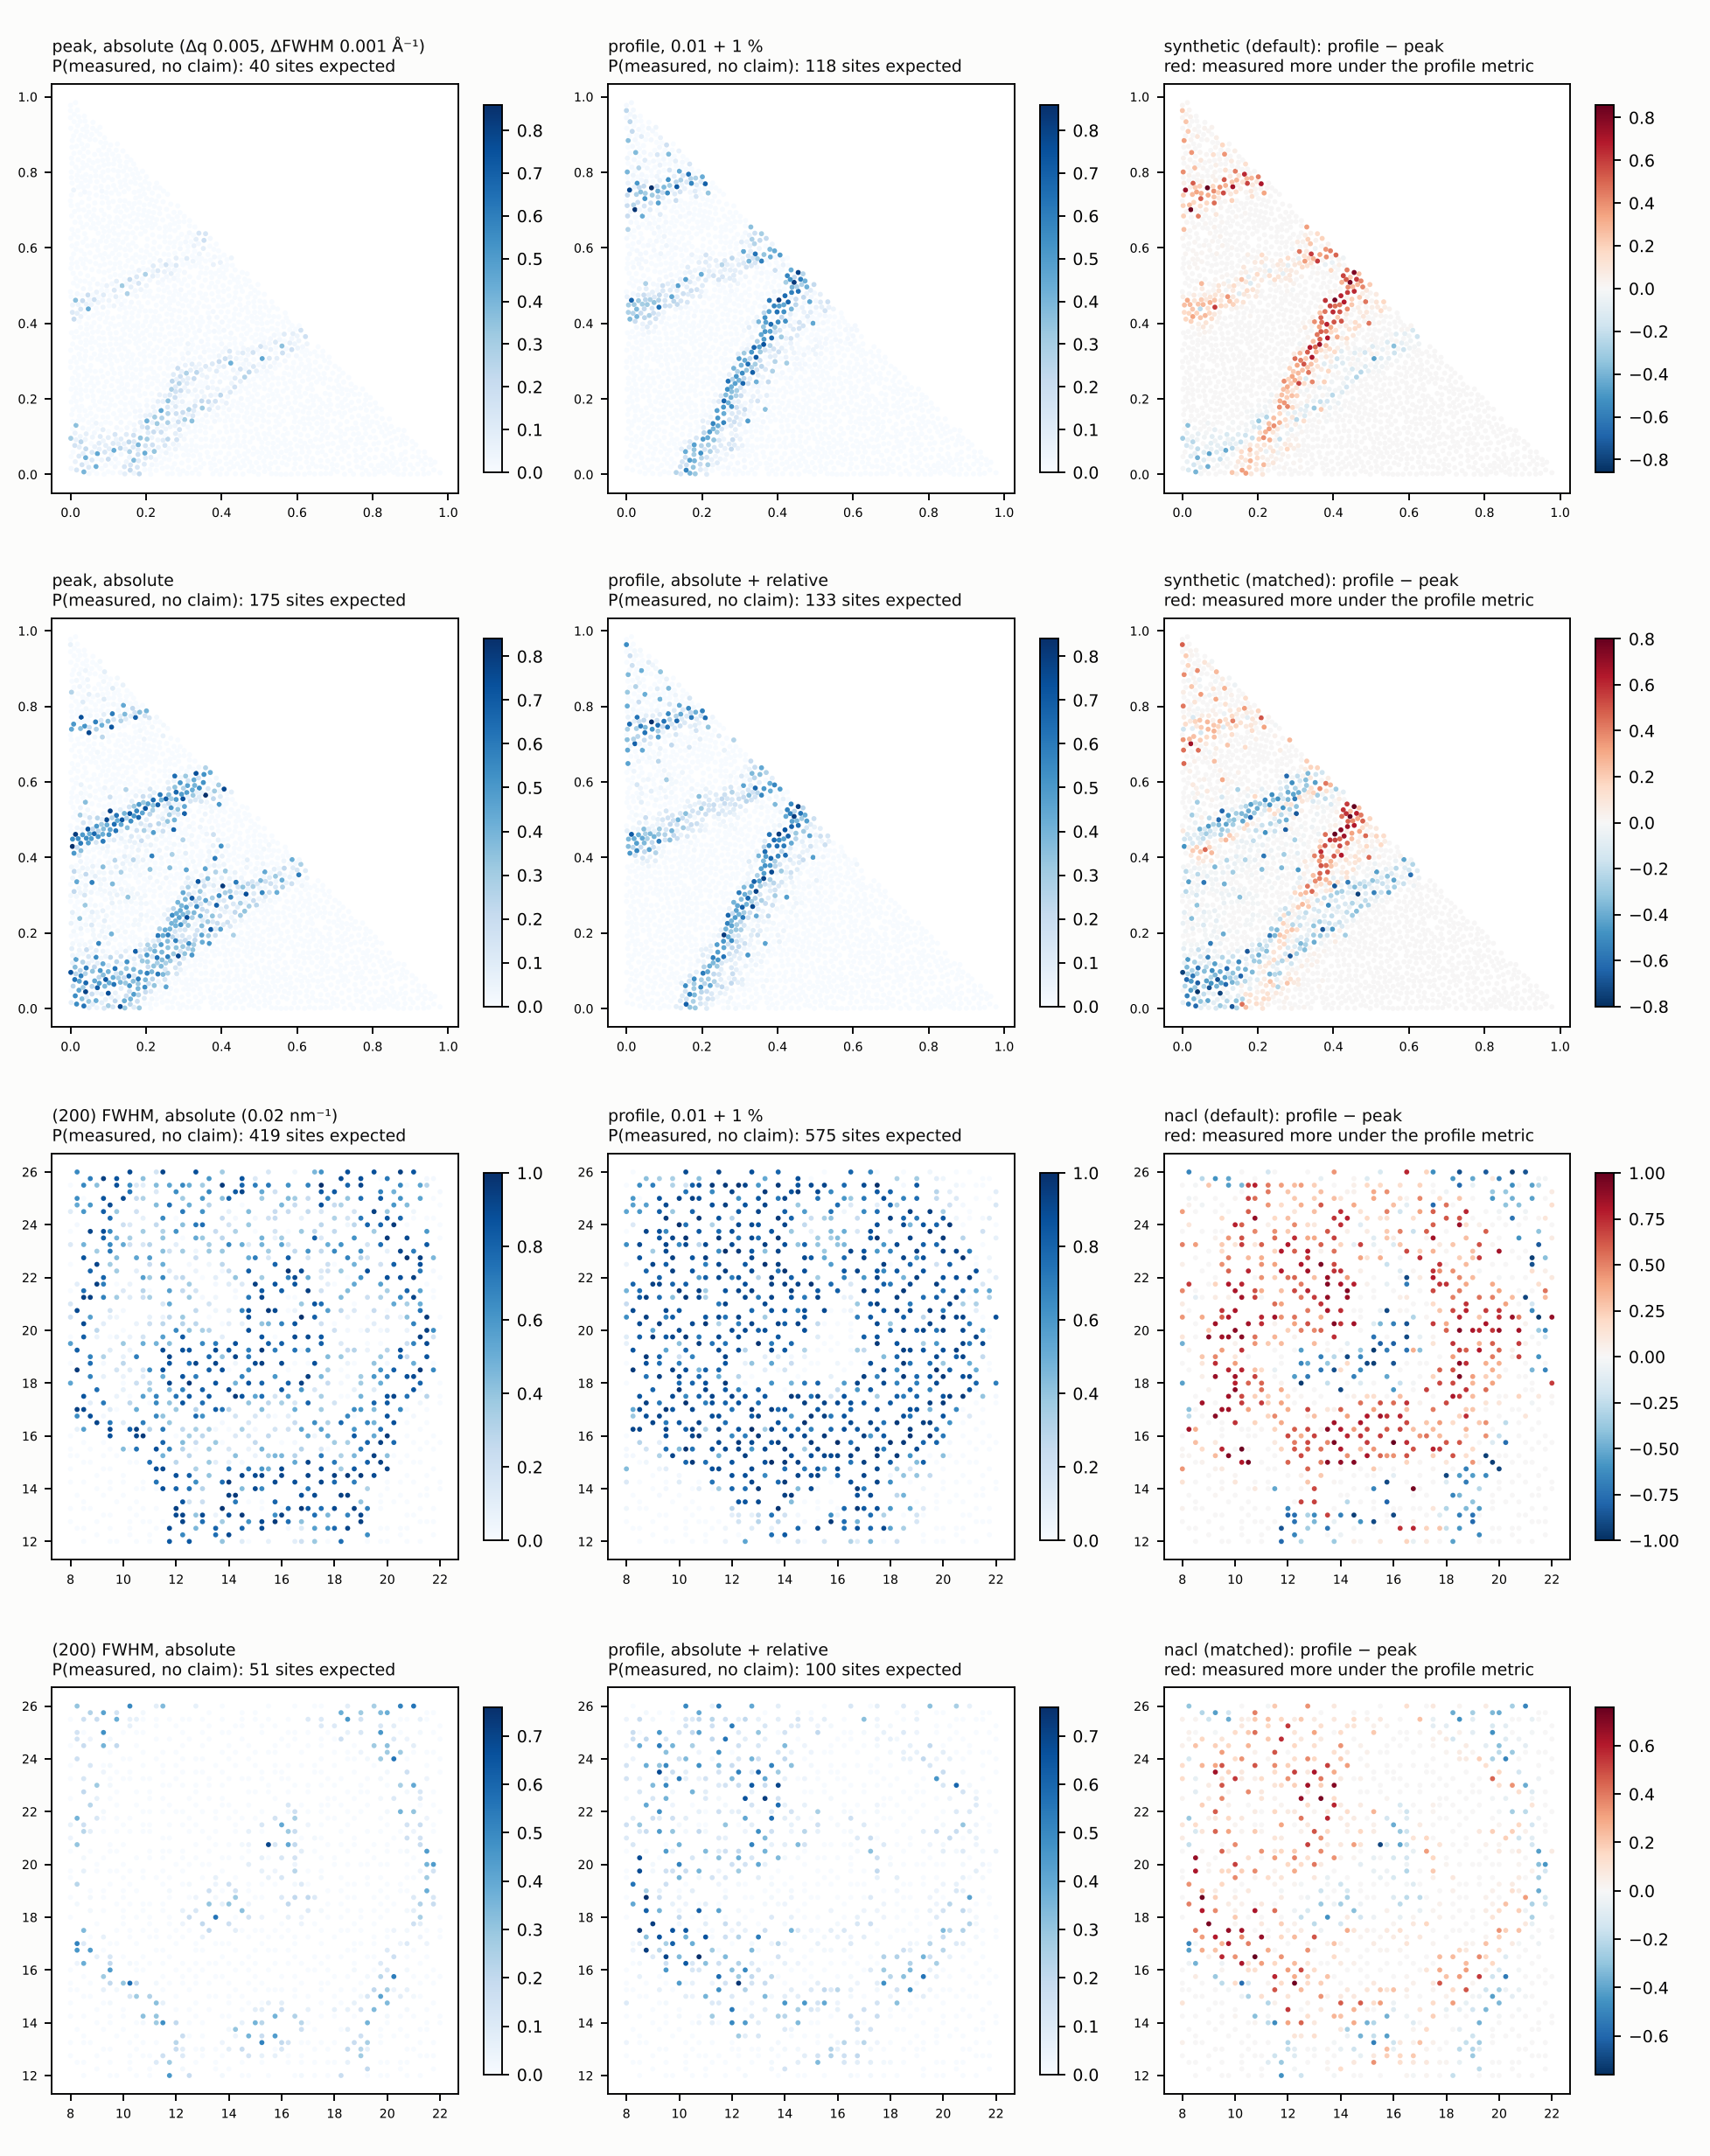
\includegraphics[width=\textwidth,height=0.44\textheight,keepaspectratio]{figures/figS6_sampling}
\caption{Frequency of measurement because no claim applied, over 50 campaigns, for the peak or line-width metric (left) and the profile metric (middle), and their difference (right; red: measured more under the profile metric). Rows: synthetic map at default and matched tolerances; NaCl scan at default and matched tolerances.}\label{fig:S6}
\end{figure}

Scripts and data: SI 4; summary in the run record, under the analysis of the metric study.

\hypertarget{si-6.2-where-wrong-interest-skips-fall-on-the-synthetic-map}{%
\subsection*{SI 6.2 Where wrong interest skips fall on the synthetic map}\label{si-6.2-where-wrong-interest-skips-fall-on-the-synthetic-map}}
\addcontentsline{toc}{subsection}{SI 6.2 Where wrong interest skips fall on the synthetic map}

This section uses a variant of the synthetic map with two claims: interest, a dominant peak at least five times its local baseline, and interpolation of the dominant-peak position and width (0.005 and 0.001 \AA{}\ensuremath{^{-1}}), at a budget of 0.20 and confidence 0.80. The main text uses the interpolation claim alone on the full profile; the records of this variant are kept in the run record and the archive of SI 5.

The skip errors of the synthetic map cluster in composition. The analysis below uses the matched-quantile rule with natural-neighbour interpolation at a budget of 0.20 and confidence 0.80; the score variants were run on the first 60 campaigns.

\begin{itemize}
\tightlist
\item
  \textbf{The guarantee held.} The record shows 161 exceedances in 1,500 level checks, against 170 allowed by the picked failure probabilities. The calibration draw is uniform within each level, so spatial correlation of the labels leaves it exchangeable with its level.
\item
  \textbf{The budget sets the count, the score the location.} Three interest scores gave about the same number of skip errors per campaign (Table S6.3). The matched-quantile rule raises its threshold until the calibration draw reaches its allowed failures, so the budget is spent whatever the score; only the sites it is spent on change.
\item
  \textbf{The recorded score depends on signal shape.} The interest label asks for a dominant peak rising above its local baseline by at least five times that baseline, a relative criterion; call the height above baseline divided by the baseline the peak-to-baseline ratio. The recorded score uses the absolute height above baseline. The broad correlation peak of the micellar phase has a high ratio to its baseline and a small absolute height (median 0.43, against 5.5 for the Bragg peaks of the ordered phases). The score therefore ranks interesting micellar sites low, and 75 \% of the wrong interest skips fall in that phase. The interpolated spectrum predicted a peak of at least five times baseline at 91 \% of these sites: the prediction was right and the score misread it.
\item
  \textbf{A score matched to the label moves the errors to the margin.} With scores based on the predicted peak-to-baseline ratio, the skip errors are the least interesting of the interesting sites (median true ratio 8.4). The probability of a skip error falls from 0.72 at ratios of 5--8 to 0.05 above 40. Such sites form contiguous bands of composition where the ratio changes slowly near the threshold, so the errors still cluster.
\item
  \textbf{The denominator matters.} The rate is taken over all sites of a level, and a third of the sites are of interest. With the recorded score, 35 \% of the interesting sites on guaranteed levels were skipped in error while every level met its budget. A bound on the share of interesting sites lost requires a label-conditional statement (Section 6, Scope of the guarantee).
\end{itemize}

{\renewcommand{\thetable}{S6.3}\small
\begin{longtable}[]{@{}
  >{\raggedright\arraybackslash}p{(\columnwidth - 6\tabcolsep) * \real{0.2500}}
  >{\raggedright\arraybackslash}p{(\columnwidth - 6\tabcolsep) * \real{0.2500}}
  >{\raggedright\arraybackslash}p{(\columnwidth - 6\tabcolsep) * \real{0.2500}}
  >{\raggedright\arraybackslash}p{(\columnwidth - 6\tabcolsep) * \real{0.2500}}@{}}
\caption{Interest scores on the synthetic map (60 campaigns, 360 level checks).}\label{tab:S6.3}\\

\toprule\noalign{}
\begin{minipage}[b]{\linewidth}\raggedright
Interest score
\end{minipage} & \begin{minipage}[b]{\linewidth}\raggedright
Skip errors per campaign
\end{minipage} & \begin{minipage}[b]{\linewidth}\raggedright
Sites measured
\end{minipage} & \begin{minipage}[b]{\linewidth}\raggedright
Exceedances
\end{minipage} \\
\midrule\noalign{}
\endhead
\bottomrule\noalign{}
\endlastfoot
Logistic on absolute peak height above baseline (recorded) & 270 & 333 & 37 / 360 \\
Logistic on peak-to-baseline ratio & 278 & 358 & 45 / 360 \\
Predicted peak-to-baseline ratio & 273 & 358 & 41 / 360 \\
\end{longtable}
}

The record keeps the original score. It meets its guarantee, and the misranking it shows is the point of this section: a score decides where the budget is spent.

\hypertarget{si-6.3-summary-of-the-metric-study}{%
\subsection*{SI 6.3 Summary of the metric study}\label{si-6.3-summary-of-the-metric-study}}
\addcontentsline{toc}{subsection}{SI 6.3 Summary of the metric study}

Six acceptance metrics were compared on the three maps with the interpolation claim alone and 50 campaigns per metric: peak or line descriptors with absolute or relative tolerance, two forms of profile envelope, and the error in a basis of the seed spectra, plain or with near-duplicate spectra merged (SI 6). Every metric kept its guarantee. Over 32 combinations of metric, dataset and tolerance, the largest ratio of observed to expected exceedances was 1.37, with a one-sided probability of 0.04 under the picked failure probabilities, the smallest of 32 such probabilities and consistent with chance; all other ratios were at most 1.08.

The metric set the cost. At tolerances a practitioner might pick, the share of sites on guaranteed levels that a prediction fails ranged from 1 \% to 85 \%, and the IR map needed between 233 and 810 measurements. Scaling every tolerance so that 15 \% of the sites fail, a control that uses the truth, brought the costs close: 338--453 sites on IR, 287--367 on NaCl and 398--461 on the synthetic map.

At equal difficulty the metric still decided where measurements go (Fig. S6). On the synthetic map the peak claim measured where the peak position and width drift with composition, in the micellar phase and in a band of the emulsion. The profile claim measured along the phase boundaries: 45--46 \% of its measurements fell on the 8.8 \% of sites next to another phase, against 32 \% for the peak claim. The two claims placed 31 \% of their measurements on the same sites, and 16 \% at the default tolerances.

The metric also decided where skip errors fall. Metrics with an absolute term put 72--83 \% of the IR skip errors on sites with signal, 30 \% of the skipped sites, and the NaCl line-width claim put 6 \% of its skip errors on sites holding the line, 66 \% of the skipped sites. Under every metric the skip errors clustered, with another skip error among the six nearest neighbours 1.5 to 3.0 times as often as for skip errors placed at random among the skipped sites. The rate also counts skip errors over all sites of a level. On the two-claim variant of the synthetic map, where a third of the sites are of interest, 35 \% of the interesting sites on guaranteed levels were skipped in error while every level met its budget (SI 6.2).

\hypertarget{si-7.-campaigns-guided-by-gaussian-process-uncertainty}{%
\section*{SI 7. Campaigns guided by Gaussian-process uncertainty}\label{si-7.-campaigns-guided-by-gaussian-process-uncertainty}}
\addcontentsline{toc}{section}{SI 7. Campaigns guided by Gaussian-process uncertainty}

Section 5.2 sets the guaranteed plan beside campaigns that skip on the strength of a model\textquotesingle s own uncertainty. The campaigns of S7.1 run on the fully measured NaCl scan with the claim on the width of the (200) line, so every skip of either can be checked afterwards. The rule without a guarantee is a skip rule on the same fixed design; campaigns driven by an acquisition function choose their sites differently and are tested in SI 10.3.

\textbf{Rule.} The campaign without a guarantee shares the hierarchical design and the seed sites of the guaranteed one. After each level from 3 on, two Gaussian processes are fitted to all sites measured so far, one to the logarithm of the width at sites with the line, one to the presence indicator at all sites; each has a squared-exponential kernel with a white-noise term, and the hyperparameters maximise the marginal likelihood \cite{RasmussenWilliams2006}. A site of the next level is skipped as having no line when the predicted presence falls below 0.1, and skipped as predictable when the predicted presence exceeds 0.9 and the interval of \(z\) standard deviations on the width lies within the tolerance of 0.02 nm\ensuremath{^{-1}}. Every other site is measured. The standard deviation is taken either for the latent function or for a new observation, which adds the fitted noise; the rule was run at \(z\) = 1, 1.64, 1.96 and 2.58. The rule involves no random draw, so each setting gives one campaign. Skip errors are counted as for the guaranteed plan: a skip for want of a line is wrong where the line is present, a predictable skip is wrong where presence disagrees or the width misses by more than the tolerance.

\textbf{Stated rate.} The process states, for every skip, its own probability that the skip is wrong. With \(p\) the predicted presence clipped to \([0, 1]\), a skip for want of a line is wrong with probability \(p\). A predictable skip is right when the line is present and the width lies within the tolerance of the predicted width \(\hat w\); with the logarithm of the width normal with mean \(\mu\) and standard deviation \(s\), latent or predictive, its probability of being wrong is

\[
1 - p \, [\Phi((\log(\hat w + t) - \mu)/s) - \Phi((\log(\hat w - t) - \mu)/s)]
\]

with \(t\) the tolerance and \(\Phi\) the standard normal distribution function. The stated share of a campaign is the sum of these probabilities over its skips on levels 3 to 6, divided by the number of sites on those levels, the quantity the guarantee bounds.

\textbf{Result.} Table S7.1 lists the eight settings. The latent standard deviation leaves out the noise that a single measurement carries, so it is the wrong quantity for a claim judged against one measurement; its rows are given for completeness. With the latent standard deviation and \(z\) = 1 the campaign measured 658 of 1071 sites, stated 3.5 \% of the sites of levels 3 to 6 wrong and skipped 10.4 \% wrongly; the shortfall was largest on the last level, 6.4 \% stated against 18 \% realised. At \(z\) of 1.64 to 2.58 it measured 893 to 903 sites, stated 0.4 \% to 0.5 \% and realised 1.0 \% to 1.4 \%. With the predictive standard deviation no interval of the width fell within the tolerance, so every skip was a skip for want of a line; the campaign measured 922 sites, stated 0.4 \% and realised 0.3 \%.

{\renewcommand{\thetable}{S7.1}\small
\begin{longtable}[]{@{}
  >{\raggedright\arraybackslash}p{(\columnwidth - 10\tabcolsep) * \real{0.1667}}
  >{\raggedright\arraybackslash}p{(\columnwidth - 10\tabcolsep) * \real{0.1667}}
  >{\raggedright\arraybackslash}p{(\columnwidth - 10\tabcolsep) * \real{0.1667}}
  >{\raggedright\arraybackslash}p{(\columnwidth - 10\tabcolsep) * \real{0.1667}}
  >{\raggedright\arraybackslash}p{(\columnwidth - 10\tabcolsep) * \real{0.1667}}
  >{\raggedright\arraybackslash}p{(\columnwidth - 10\tabcolsep) * \real{0.1667}}@{}}
\caption{Campaigns without a guarantee on the NaCl (200)-width map. Stated and realised shares are of the sites of levels 3 to 6.}\label{tab:S7.1}\\

\toprule\noalign{}
\begin{minipage}[b]{\linewidth}\raggedright
standard deviation
\end{minipage} & \begin{minipage}[b]{\linewidth}\raggedright
\(z\)
\end{minipage} & \begin{minipage}[b]{\linewidth}\raggedright
measured
\end{minipage} & \begin{minipage}[b]{\linewidth}\raggedright
predictable skips
\end{minipage} & \begin{minipage}[b]{\linewidth}\raggedright
stated share wrong
\end{minipage} & \begin{minipage}[b]{\linewidth}\raggedright
realised share wrong
\end{minipage} \\
\midrule\noalign{}
\endhead
\bottomrule\noalign{}
\endlastfoot
latent & 1.00 & 658 & 266 & 3.5 \% & 10.4 \% \\
latent & 1.64 & 893 & 31 & 0.5 \% & 1.4 \% \\
latent & 1.96 & 903 & 21 & 0.4 \% & 1.0 \% \\
latent & 2.58 & 903 & 21 & 0.4 \% & 1.0 \% \\
predictive & 1.00--2.58 & 922 & 0 & 0.4 \% & 0.3 \% \\
\end{longtable}
}

The guarantee applies to the Gaussian process as it does to natural-neighbour prediction. With the posterior mean as the frozen predictor and the length scale set by maximum likelihood, by the design or by the nonstationary rule (SI 1), 250 guaranteed campaigns each skipped 12.3 \% to 12.5 \% of levels 3 to 6 wrongly on average and exceeded the budget on 111 to 123 of 1000 level runs, against 120 expected; they measured 745 to 777 sites, against 614 with natural-neighbour prediction, because the posterior mean shrinks toward the average where the width scatters from site to site. The guaranteed Gaussian process measured fewer sites than the one without a guarantee with the predictive standard deviation, 745 to 777 against 922, and its rate was fixed before any skip was checked; the campaigns without a guarantee learn their realised rate only from the full scan that a campaign exists to avoid.

The comparison can hold model and ranking fixed (Fig. S7b). With the process refitted after each level, predicting the full profile, and its own posterior probability of a skip error as the frozen score, a guaranteed plan measured 761 \ensuremath{\pm} 68 of 1071 sites over 50 campaigns and exceeded the budget on 16 of 200 level checks, against 24 expected; skipping where that same probability was at most \ensuremath{\alpha}, for \ensuremath{\alpha} from 0.01 to 0.32, the process measured 1064 to 1070.

\begin{figure}[tbp]\renewcommand{\thefigure}{S7b}
\centering
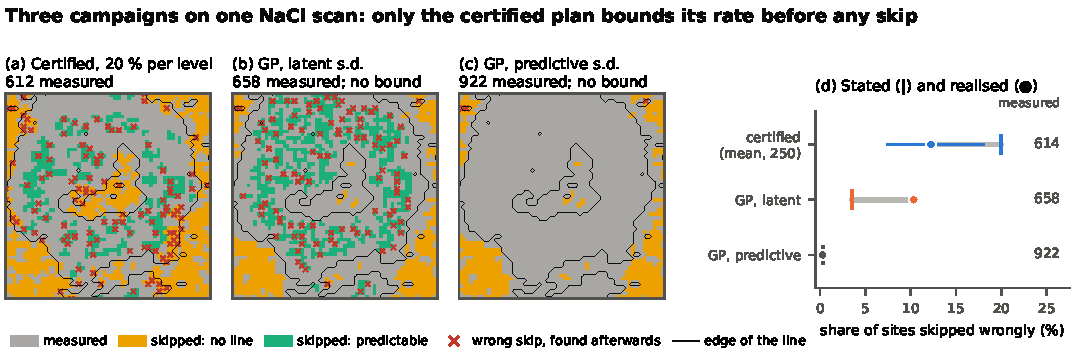
\includegraphics[width=\textwidth,height=0.44\textheight,keepaspectratio]{figures/fig_hook_three}
\caption{One Gaussian process on the NaCl scan, claim on the width of the (200) line, 1071 design sites. (a) A guaranteed plan of average cost with the process as predictor and its own posterior probability of a skip error as the frozen score: at most 20 \% of each level skipped in error, with confidence 0.80 for that level. (b) The same process skipping a site when that probability is at most \ensuremath{\alpha} = 0.20. Crosses mark skip errors, found afterwards against the full scan. (c) Share of the sites on guaranteed levels skipped in error: stated in advance (bar) and realised (dot), with sites measured. For the process without a guarantee the statement is its own probability summed over its skips; for the guaranteed plans it is the bound, with the mean and 5--95 \% range of 50 campaigns with the process and 250 with natural-neighbour prediction.}\label{fig:S7b}
\end{figure}

\hypertarget{s7.2-the-spectrum-gaussian-process-on-all-three-maps}{%
\subsection*{S7.2 The spectrum Gaussian process on all three maps}\label{s7.2-the-spectrum-gaussian-process-on-all-three-maps}}
\addcontentsline{toc}{subsection}{S7.2 The spectrum Gaussian process on all three maps}

The rule of Section 5.2 uses the Gaussian process of the guaranteed campaigns (Section 4.3), which predicts the full spectrum or profile at a site from the measured set. After each level is measured, the process is refitted with the length scale set by maximum marginal likelihood, and every unmeasured site of the next level is assessed against both claims. The process places one length scale on all channels, so a posterior over the claims needs a model of how channels vary together; here posterior draws of the spectrum at a site are taken along the leading principal components of the measured spectra, which carry 99 \% of the variance up to at most 20 components, with the component variances scaled by the posterior standard deviation at the site; 64 draws per site, clipped at zero. This construction is one choice among several, and the stated rates of Table S7.2 belong to it; another posterior over the claims would state other rates. The stated probability that a claim fails at a site is the share of draws for which it fails: for the interest claim, the share of draws that are of interest; for the interpolation claim, the share of draws that fail the acceptance metric against the posterior mean. A site is skipped under a claim when its stated probability is at most \ensuremath{\alpha}, and a site skipped under both claims is stated to fail with probability \(1 - (1 - p_a)(1 - p_b)\). The stated share of skip errors of a campaign is the sum of these probabilities over its skipped sites on guaranteed levels, divided by the number of sites on guaranteed levels.

Three standard deviations are used: the latent one, the predictive one, which adds the fitted noise variance, and the predictive one multiplied by a factor fixed on each level from the measured set, the 68 \% quantile of the absolute leave-one-out residuals in units of their predictive standard deviation. A factor below one means the measured sites are predicted better than the process states, and the rescaled campaign then skips more.

{\renewcommand{\thetable}{S7.2}\small
\begin{longtable}[]{@{}
  >{\raggedright\arraybackslash}p{(\columnwidth - 8\tabcolsep) * \real{0.2000}}
  >{\raggedright\arraybackslash}p{(\columnwidth - 8\tabcolsep) * \real{0.2000}}
  >{\raggedright\arraybackslash}p{(\columnwidth - 8\tabcolsep) * \real{0.2000}}
  >{\raggedright\arraybackslash}p{(\columnwidth - 8\tabcolsep) * \real{0.2000}}
  >{\raggedright\arraybackslash}p{(\columnwidth - 8\tabcolsep) * \real{0.2000}}@{}}
\caption{Spectrum Gaussian-process campaigns without a guarantee, ranges over \ensuremath{\alpha} from 0.01 to 0.32. Shares are of the sites on guaranteed levels.}\label{tab:S7.2}\\

\toprule\noalign{}
\begin{minipage}[b]{\linewidth}\raggedright
map
\end{minipage} & \begin{minipage}[b]{\linewidth}\raggedright
standard deviation
\end{minipage} & \begin{minipage}[b]{\linewidth}\raggedright
stated share wrong
\end{minipage} & \begin{minipage}[b]{\linewidth}\raggedright
realised share wrong
\end{minipage} & \begin{minipage}[b]{\linewidth}\raggedright
measured
\end{minipage} \\
\midrule\noalign{}
\endhead
\bottomrule\noalign{}
\endlastfoot
IR (959 sites) & latent & 0--7.4 \% & 1.0--3.3 \% & 73--191 \\
& predictive & 0--9.1 \% & 0.7--2.3 \% & 73--398 \\
& rescaled (factor 0.40) & 0--3.7 \% & 1.6--4.5 \% & 73--75 \\
NaCl (1071 sites) & latent & 0--0.7 \% & 0.1--1.6 \% & 1042--1070 \\
& predictive & 0--0.1 \% & 0.1--0.4 \% & 1064--1070 \\
& rescaled (factor 0.19--0.89) & 0--2.1 \% & 0.1--5.8 \% & 959--1070 \\
synthetic (2118 sites) & latent & 0--0.1~\% & 0~\% & 2109--2118 \\
& predictive & 0~\% & 0~\% & 2118 \\
& rescaled (factor 0.06--0.23) & 0--1.8~\% & 0.3--2.1~\% & 1506--1792 \\
\end{longtable}
}

On IR, 73 sites form the seed, so a campaign at 73 measured sites skipped every guaranteed-level site. On the synthetic map the claim is on the full profile at 0.5~\% + 0.005; the process judged every site too uncertain to skip at every \ensuremath{\alpha}, and only the rescaled process skipped. The two-claim variant of SI 6.2, with its peak claim, gave stated shares of at most 4~\% against realised shares of 11~\% to 41~\%; those runs are kept in the archive of SI 5. On NaCl the fitted white-noise variance, about three quarters of the variance of the width, makes the predictive process unwilling to skip; it describes site-to-site scatter that the smooth part of the process does not follow, far above the counting noise of a measurement (SI 2).

\textbf{The same process, guaranteed.} The frozen interpolation score of a guaranteed plan can be the process\textquotesingle s own posterior probability of a skip error, computed as above with the predictive standard deviation before each calibration draw, from the measured set only and with a fixed random stream; ties among the 64-draw probabilities are broken by the mean deviation of the draws. The predictor is the process\textquotesingle s posterior mean, the length scale set by maximum likelihood, the budget that of Table 3. On NaCl, 50 campaigns measured 761 \ensuremath{\pm} 68 of 1071 sites, with 16 of 200 level checks over budget against 24.0 expected under the picked failure probabilities; the rule without a guarantee, with the same process and the same probability measured 1064 to 1070 (Table S7.2). On the synthetic map, 20 campaigns measured 1991 \ensuremath{\pm} 91 of 2118, with 13 of 120 level checks over budget against 11.4 expected, against 2118 without a guarantee. The ranking saved nothing over the positional standard deviation of Section 4.3 (745 to 777 on NaCl, 1946 to 2027 on the synthetic map). The process mean failed at 74~\% and 77~\% of the calibration sites of the two maps, against 52~\% and 40~\% for natural-neighbour prediction.

\hypertarget{s7.3-guaranteed-campaigns-at-several-budgets}{%
\subsection*{S7.3 Guaranteed campaigns at several budgets}\label{s7.3-guaranteed-campaigns-at-several-budgets}}
\addcontentsline{toc}{subsection}{S7.3 Guaranteed campaigns at several budgets}

For Fig. 4 the matched-quantile rule was run at budgets \(\varepsilon\) of 0.05, 0.10, 0.20 and 0.30 on the shared skip-error rate, at the confidences of Section 4.3, with natural-neighbour prediction (20 campaigns per budget) and Gaussian-process prediction with the length scale by maximum likelihood (8 campaigns per budget, 4 on the synthetic map).

{\renewcommand{\thetable}{S7.3}\small
\begin{longtable}[]{@{}
  >{\raggedright\arraybackslash}p{(\columnwidth - 10\tabcolsep) * \real{0.1667}}
  >{\raggedright\arraybackslash}p{(\columnwidth - 10\tabcolsep) * \real{0.1667}}
  >{\raggedright\arraybackslash}p{(\columnwidth - 10\tabcolsep) * \real{0.1667}}
  >{\raggedright\arraybackslash}p{(\columnwidth - 10\tabcolsep) * \real{0.1667}}
  >{\raggedright\arraybackslash}p{(\columnwidth - 10\tabcolsep) * \real{0.1667}}
  >{\raggedright\arraybackslash}p{(\columnwidth - 10\tabcolsep) * \real{0.1667}}@{}}
\caption{Guaranteed campaigns by budget: sites measured (mean \ensuremath{\pm} standard deviation) and, in brackets, the mean realised share of the sites on guaranteed levels skipped in error. NN, natural-neighbour prediction; GP, Gaussian-process prediction.}\label{tab:S7.3}\\

\toprule\noalign{}
\begin{minipage}[b]{\linewidth}\raggedright
map
\end{minipage} & \begin{minipage}[b]{\linewidth}\raggedright
predictor
\end{minipage} & \begin{minipage}[b]{\linewidth}\raggedright
\ensuremath{\varepsilon} = 0.05
\end{minipage} & \begin{minipage}[b]{\linewidth}\raggedright
\ensuremath{\varepsilon} = 0.10
\end{minipage} & \begin{minipage}[b]{\linewidth}\raggedright
\ensuremath{\varepsilon} = 0.20
\end{minipage} & \begin{minipage}[b]{\linewidth}\raggedright
\ensuremath{\varepsilon} = 0.30
\end{minipage} \\
\midrule\noalign{}
\endhead
\bottomrule\noalign{}
\endlastfoot
IR & NN & 473 \ensuremath{\pm} 70 (1.5~\%) & 312 \ensuremath{\pm} 58 (3.4~\%) & 233 \ensuremath{\pm} 1 (4.1~\%) & 233 \ensuremath{\pm} 0 (4.1~\%) \\
& GP & 410 \ensuremath{\pm} 66 (1.5~\%) & 271 \ensuremath{\pm} 31 (3.7~\%) & 233 \ensuremath{\pm} 1 (4.3~\%) & 233 \ensuremath{\pm} 0 (4.3~\%) \\
NaCl & NN & 898 \ensuremath{\pm} 52 (1.9~\%) & 806 \ensuremath{\pm} 69 (4.5~\%) & 631 \ensuremath{\pm} 69 (11.5~\%) & 484 \ensuremath{\pm} 47 (19.9~\%) \\
& GP & 1022 \ensuremath{\pm} 23 (2.2~\%) & 963 \ensuremath{\pm} 54 (4.2~\%) & 767 \ensuremath{\pm} 69 (11.5~\%) & 624 \ensuremath{\pm} 65 (18.3~\%) \\
synthetic & NN & 1128 \ensuremath{\pm} 229 (2.2~\%) & 918 \ensuremath{\pm} 219 (4.5~\%) & 542 \ensuremath{\pm} 83 (12.5~\%) & 392 \ensuremath{\pm} 57 (20.3~\%) \\
& GP & 2061 \ensuremath{\pm} 24 (1.8~\%) & 1940 \ensuremath{\pm} 95 (5.8~\%) & 1673 \ensuremath{\pm} 138 (14.3~\%) & 1460 \ensuremath{\pm} 122 (22.4~\%) \\
\end{longtable}
}

On IR, 233 sites is the floor: 73 seed sites and 160 calibration draws. Above a budget of 0.10 every predicted skip is admitted, and the realised share stays at the rate the predictor makes.

\begin{figure}[tbp]\renewcommand{\thefigure}{S7}
\centering
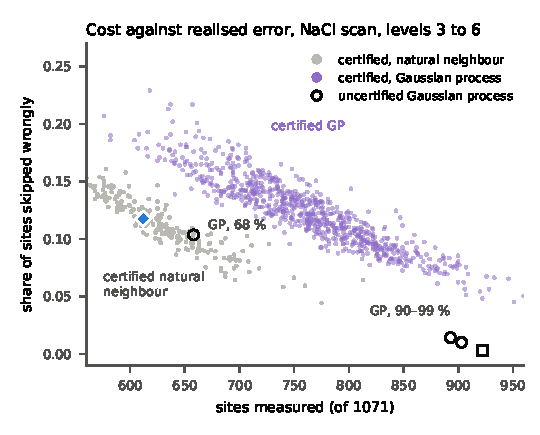
\includegraphics[width=\textwidth,height=0.44\textheight,keepaspectratio]{figures/figS7_cost}
\caption{The NaCl scan, levels 3 to 6. (a) Sites measured against the share of sites skipped in error: 250 guaranteed campaigns with natural-neighbour prediction (grey; diamond: random state 44), 3 \ensuremath{\times} 250 guaranteed campaigns with the Gaussian-process mean as predictor (purple; length scale by maximum likelihood, by design spacing or by local spacing), and the Gaussian-process rule without a guarantee at intervals of 68 \% to 99 \% (open symbols). (b) Realised share of each level skipped in error in the 250 guaranteed campaigns of natural-neighbour prediction, against the budget of 20 \%; numbers give level runs over budget against the number expected under the picked failure probabilities.}\label{fig:S7}
\end{figure}

\hypertarget{s7.4-the-paired-comparison-of-fig.-1}{%
\subsection*{S7.4 The paired comparison of Fig. 1}\label{s7.4-the-paired-comparison-of-fig.-1}}
\addcontentsline{toc}{subsection}{S7.4 The paired comparison of Fig. 1}

The comparison of Fig. 1 holds design, model, ranking and calibration sample fixed and varies only the cut on the sites left after calibration (Section 4.3). Designs are drawn with the hierarchical Poisson-disk sampler at radii 0.2/\ensuremath{\surd}2\^{}l mm for levels l = 0 to 6, corners forced, and snapped to the NaCl raster (seeds 1000 to 1079); levels 0 to 3 form the seed. Each round fits two Gaussian processes on all sites measured so far: presence of the (200) line, regressed as 0 or 1 and clipped to {[}0, 1{]}, and the logarithm of its width at measured sites that hold the line. Both use a squared-exponential kernel with an output scale and a white-noise term, outputs standardised, two restarts of the optimiser. A site is predicted to hold the line when the presence prediction is at least 0.5. Its probability of a skip error is one minus the product of the presence prediction and the predictive probability that the width lies within the tolerance when the line is predicted, and the presence prediction otherwise. The calibration sample of 40 sites is drawn with its own random stream, identical in both cuts of a design.

The uncertainty of the model is turned into a statement on the number of skip errors by 2000 joint draws: presence is drawn site by site with the predicted probability, and log width jointly over the remaining sites from the full predictive covariance. The cut is the longest prefix of the ranking for which at least 80 \% of the draws stay within \(\lfloor 0.2 N \rfloor\) skip errors, \(N\) the size of the round, and the stated rate is the 80 \% quantile of the draws at that prefix, divided by \(N\). The conformal cut scans thresholds on the same probability in increasing order and keeps the largest for which the exact hypergeometric upper limit at confidence 0.80 on the number of failures in the round, given the calibration failures below the threshold, less those failures, is at most \(\lfloor 0.2 N \rfloor\); the stated rate is that difference divided by \(N\). A cut keeps its rate in a campaign when the realised skip errors among the sites it skips, divided by \(N\), are at most its stated rate. Presence is regressed on 0 and 1 for speed; a classifier would change the ranking and the model\textquotesingle s statement and leave the conformal guarantee unchanged.

The three kernels differ only in two settings. With the noise level fitted, the white-noise term is optimised between 10\ensuremath{^{-}}\ensuremath{^{4}} and 10 of the standardised variance. With the noise fixed, the term is held at 10\ensuremath{^{-}}\ensuremath{^{4}}. With the long length scale, the term is held at 10\ensuremath{^{-}}\ensuremath{^{4}} and the length scale bounded below by 1 mm; maximum likelihood with the noise fitted gives about 0.23 mm. The random predictor copies, for each site of a round, the presence and width of a measured site chosen uniformly at random and ranks the sites by independent uniform numbers.

{\renewcommand{\thetable}{S7.4}\small
\begin{longtable}[]{@{}
  >{\raggedright\arraybackslash}p{(\columnwidth - 10\tabcolsep) * \real{0.1667}}
  >{\raggedright\arraybackslash}p{(\columnwidth - 10\tabcolsep) * \real{0.1667}}
  >{\raggedright\arraybackslash}p{(\columnwidth - 10\tabcolsep) * \real{0.1667}}
  >{\raggedright\arraybackslash}p{(\columnwidth - 10\tabcolsep) * \real{0.1667}}
  >{\raggedright\arraybackslash}p{(\columnwidth - 10\tabcolsep) * \real{0.1667}}
  >{\raggedright\arraybackslash}p{(\columnwidth - 10\tabcolsep) * \real{0.1667}}@{}}
\caption{The paired comparison, 80 designs per row. Drive: the cut whose skips decide what is measured next; cut: the cut evaluated on the same states. Within rate: share of campaigns (\%) whose realised skip errors stayed within the rate stated before the round, rounds 1 / 2 / 3, against a target of 80 \% (a method meeting it exactly gives 71 \% to 89 \% in 95 of 100 such sets). Skip errors: mean skip errors of mean skips per round. Measured: mean sites measured by the driven campaign, seed and calibration included, of about 1075.}\label{tab:S7.4}\\

\toprule\noalign{}
\begin{minipage}[b]{\linewidth}\raggedright
kernel
\end{minipage} & \begin{minipage}[b]{\linewidth}\raggedright
drive
\end{minipage} & \begin{minipage}[b]{\linewidth}\raggedright
cut
\end{minipage} & \begin{minipage}[b]{\linewidth}\raggedright
within rate
\end{minipage} & \begin{minipage}[b]{\linewidth}\raggedright
skip errors
\end{minipage} & \begin{minipage}[b]{\linewidth}\raggedright
measured
\end{minipage} \\
\midrule\noalign{}
\endhead
\bottomrule\noalign{}
\endlastfoot
noise level fitted & model & model & 87.5 / 98.8 / 100.0 & 21 of 68 / 40 of 150 / 76 of 314 & 543 \\
& model & thresholds & 77.5 / 85.0 / 81.2 & 20 of 65 / 38 of 143 / 66 of 287 & 543 \\
& thresholds & model & 87.5 / 97.5 / 100.0 & 21 of 68 / 40 of 150 / 77 of 316 & 580 \\
& thresholds & thresholds & 77.5 / 83.8 / 82.5 & 20 of 65 / 38 of 144 / 66 of 286 & 580 \\
noise fixed at 10\ensuremath{^{-}}\ensuremath{^{4}} & model & model & 73.8 / 68.8 / 88.8 & 24 of 75 / 50 of 165 / 93 of 336 & 500 \\
& model & thresholds & 82.5 / 81.2 / 88.8 & 19 of 61 / 37 of 132 / 66 of 269 & 500 \\
& thresholds & model & 73.8 / 77.5 / 85.0 & 24 of 75 / 49 of 163 / 94 of 338 & 619 \\
& thresholds & thresholds & 82.5 / 88.8 / 88.8 & 19 of 61 / 35 of 129 / 65 of 266 & 619 \\
length scale \ensuremath{\ge} 1 mm & model & model & 0.0 / 0.0 / 0.0 & 42 of 93 / 102 of 222 / 204 of 443 & 317 \\
& model & thresholds & 87.5 / 77.5 / 83.8 & 19 of 53 / 38 of 108 / 69 of 206 & 317 \\
& thresholds & model & 0.0 / 0.0 / 0.0 & 42 of 93 / 104 of 222 / 229 of 447 & 723 \\
& thresholds & thresholds & 87.5 / 81.2 / 77.5 & 19 of 53 / 36 of 103 / 72 of 196 & 723 \\
random predictor & thresholds & thresholds & 80.0 / 78.8 / 82.5 & 21 of 31 / 38 of 56 / 67 of 97 & 891 \\
\end{longtable}
}

Map quality was compared on 20 designs with the noise level fitted and with the long length scale. Each measured set, and a control of the seed plus a uniform random draw of the other design sites of equal size, was refitted with a Gaussian-process classifier for presence and a Gaussian-process regression for the log width with fitted white noise, both with a Matérn kernel of smoothness ½; on the seven sets of design 0, marginal likelihood preferred smoothness 5/2 on every set, which predicted the raster worse by 0.4 to 6 percentage points. The error is the share of the 3249 raster sites at which presence is predicted wrongly or the width is off by more than the tolerance.

{\renewcommand{\thetable}{S7.5}\small
\begin{longtable}[]{@{}
  >{\raggedright\arraybackslash}p{(\columnwidth - 8\tabcolsep) * \real{0.2000}}
  >{\raggedright\arraybackslash}p{(\columnwidth - 8\tabcolsep) * \real{0.2000}}
  >{\raggedright\arraybackslash}p{(\columnwidth - 8\tabcolsep) * \real{0.2000}}
  >{\raggedright\arraybackslash}p{(\columnwidth - 8\tabcolsep) * \real{0.2000}}
  >{\raggedright\arraybackslash}p{(\columnwidth - 8\tabcolsep) * \real{0.2000}}@{}}
\caption{Map quality after round 3, mean over 20 designs: share of the raster outside tolerance (\%), with presence wrong in brackets.}\label{tab:S7.5}\\

\toprule\noalign{}
\begin{minipage}[b]{\linewidth}\raggedright
kernel
\end{minipage} & \begin{minipage}[b]{\linewidth}\raggedright
drive
\end{minipage} & \begin{minipage}[b]{\linewidth}\raggedright
sites measured
\end{minipage} & \begin{minipage}[b]{\linewidth}\raggedright
measured set
\end{minipage} & \begin{minipage}[b]{\linewidth}\raggedright
random set of equal size
\end{minipage} \\
\midrule\noalign{}
\endhead
\bottomrule\noalign{}
\endlastfoot
noise level fitted & model & 538 & 25.9 (5.3) & 26.9 (6.2) \\
& thresholds & 562 & 26.0 (5.3) & 27.3 (6.1) \\
length scale \ensuremath{\ge} 1 mm & model & 312 & 29.9 (7.7) & 30.5 (8.2) \\
& thresholds & 720 & 24.0 (4.7) & 25.3 (5.1) \\
\end{longtable}
}

\begin{figure}[tbp]\renewcommand{\thefigure}{S7c}
\centering
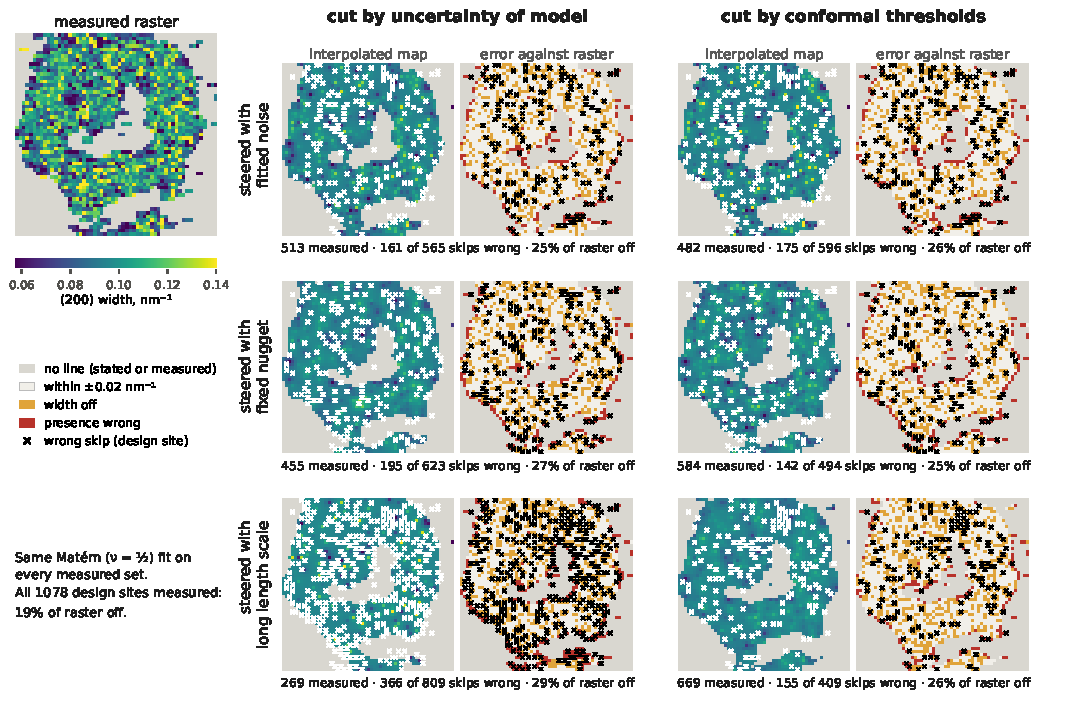
\includegraphics[width=\textwidth,height=0.44\textheight,keepaspectratio]{figures/figS_paired_maps_matern}
\caption{Maps after round 3 of one paired design (design 0), refitted with the Matérn model of Table S7.5. Rows: the kernel that steered the campaign; columns: the cut that drove it, with the interpolated width and its error against the raster. Crosses mark the campaign\textquotesingle s skip errors. Measuring every site of this design leaves 19 \% of the raster outside tolerance.}\label{fig:S7c}
\end{figure}

Code and records: \texttt{experiments/paired\_gp.py}, \texttt{experiments/chicken.py}, \texttt{experiments/paired\_gp\_fitquality.py}, \texttt{experiments/paired\_gp\_maps.py}, \texttt{experiments/paired\_gp\_bestfit.py}; \texttt{results/revision2/paired\_gp.jsonl}, \texttt{paired\_chicken.jsonl}, \texttt{paired\_gp\_fitquality.jsonl}, \texttt{paired\_gp\_summary.json}. Fig. 1 is drawn by \texttt{manuscript/figures/fig\_hook4.py}.

\hypertarget{si-8.-the-record-of-measured-sites}{%
\section*{SI 8. The record of measured sites}\label{si-8.-the-record-of-measured-sites}}
\addcontentsline{toc}{section}{SI 8. The record of measured sites}

A guaranteed skip carries its claim and its bound; a guaranteed measurement can carry a record of equal standing. Every site of a guaranteed level is decided from a frozen prediction, a score per claim and the guaranteed cut of its level, so the reason for a measurement is fixed before the measurement is taken. The measurement then adds the outcome, and the record shows whether the site was needed.

\textbf{The record.} Table S8.1 lists the entries kept for each design site. The decision entries are written before the site is measured or skipped; the outcome entries follow from the measurement, for skipped sites from the full scan available in a retrospective study. The residual is the departure of the frozen prediction from the measurement in units of the tolerance, so that a skip under the interpolation claim fails above one; where the presence of the feature decides, agreed absence counts as zero and disagreement as infinite. The quantile of a residual is its randomised conformal p-value among the calibration residuals of the same level \cite{Vovk2005}: the share of calibration residuals above it, with ties broken by a uniform draw. A p-value below 0.2 places a residual among the largest fifth of the calibration residuals of its level. Calibration sites are a uniform draw from their level, so each fifth would hold 20 \% of the sites measured by choice if the score carried no information; the largest fifth holds more to the degree that the score finds the sites the prediction misses.

{\renewcommand{\thetable}{S8.1}\small
\begin{longtable}[]{@{}
  >{\raggedright\arraybackslash}p{(\columnwidth - 4\tabcolsep) * \real{0.3333}}
  >{\raggedright\arraybackslash}p{(\columnwidth - 4\tabcolsep) * \real{0.3333}}
  >{\raggedright\arraybackslash}p{(\columnwidth - 4\tabcolsep) * \real{0.3333}}@{}}
\caption{Entries of the record of each design site.}\label{tab:S8.1}\\

\toprule\noalign{}
\begin{minipage}[b]{\linewidth}\raggedright
entry
\end{minipage} & \begin{minipage}[b]{\linewidth}\raggedright
written
\end{minipage} & \begin{minipage}[b]{\linewidth}\raggedright
content
\end{minipage} \\
\midrule\noalign{}
\endhead
\bottomrule\noalign{}
\endlastfoot
level & before & level of the hierarchical design \\
action & before & measured as seed, as calibration draw or by choice (no claim covers the site); skipped as not of interest, as predictable or both \\
score, cut & before & score of each claim and the guaranteed cut of the level; a claim covers the site when its score is at or below the cut \\
margin, rank & before & score minus cut; rank of the score within the level \\
prediction & before & frozen prediction of the feature (presence, width, peak position or band envelope) \\
measurement & after & measured feature \\
residual & after & departure of the prediction from the measurement, in tolerances \\
labels & after & the prediction fails (residual above one); the site is of interest \\
p-value & after & randomised conformal p-value of the residual among the calibration residuals of the level \\
\end{longtable}
}

\textbf{Campaigns.} The record was written for one campaign of average cost per dataset, replayed from its recorded random state: for the NaCl scan the campaign of random state 44, for the IR map and the synthetic map the campaign whose number of measurements lies closest to the mean of 250, with ties broken by the number of skip errors. Each replay reproduced the recorded actions site by site. The failure and interest labels are part of the record of all 250 campaigns per dataset, so the shares in Table S8.2 pool those campaigns; the p-values come from the replayed campaigns. A site measured by choice is needed when every claim would have skipped it wrongly, that is when it is of interest and its prediction fails.

{\renewcommand{\thetable}{S8.2}\small
\begin{longtable}[]{@{}
  >{\raggedright\arraybackslash}p{(\columnwidth - 14\tabcolsep) * \real{0.1250}}
  >{\raggedright\arraybackslash}p{(\columnwidth - 14\tabcolsep) * \real{0.1250}}
  >{\raggedright\arraybackslash}p{(\columnwidth - 14\tabcolsep) * \real{0.1250}}
  >{\raggedright\arraybackslash}p{(\columnwidth - 14\tabcolsep) * \real{0.1250}}
  >{\raggedright\arraybackslash}p{(\columnwidth - 14\tabcolsep) * \real{0.1250}}
  >{\raggedright\arraybackslash}p{(\columnwidth - 14\tabcolsep) * \real{0.1250}}
  >{\raggedright\arraybackslash}p{(\columnwidth - 14\tabcolsep) * \real{0.1250}}
  >{\raggedright\arraybackslash}p{(\columnwidth - 14\tabcolsep) * \real{0.1250}}@{}}
\caption{Measured sites at the guaranteed levels. Sites: design sites of the guaranteed levels; drawn, chosen: calibration draws and sites measured by choice per campaign; fails, of interest, needed: shares among sites drawn / chosen. Counts and shares pool 250 campaigns per dataset. The last column, the share of sites measured by choice whose residual lies among the largest fifth of the calibration residuals of its level, comes from the replayed campaign and equals 0.20 for a score without information.}\label{tab:S8.2}\\

\toprule\noalign{}
\begin{minipage}[b]{\linewidth}\raggedright
dataset
\end{minipage} & \begin{minipage}[b]{\linewidth}\raggedright
sites
\end{minipage} & \begin{minipage}[b]{\linewidth}\raggedright
drawn
\end{minipage} & \begin{minipage}[b]{\linewidth}\raggedright
chosen
\end{minipage} & \begin{minipage}[b]{\linewidth}\raggedright
fails
\end{minipage} & \begin{minipage}[b]{\linewidth}\raggedright
of interest
\end{minipage} & \begin{minipage}[b]{\linewidth}\raggedright
needed
\end{minipage} & \begin{minipage}[b]{\linewidth}\raggedright
largest fifth
\end{minipage} \\
\midrule\noalign{}
\endhead
\bottomrule\noalign{}
\endlastfoot
NaCl width & 995 & 160 & 378 & 0.52/0.60 & 0.66/0.86 & 0.35/0.47 & 0.18 \\
IR amide I & 886 & 160 & 62 & 0.014/0.021 & 0.38/0.79 & 0.013/0.019 & 0.21 \\
synthetic profile & 2079 & 233 & 660 & 0.40/0.43 & all & 0.40/0.43 & 0.35 \\
\end{longtable}
}

\textbf{What the record shows.} On the synthetic map every site is of interest and the tight profile claim fails at 40 \% of sites drawn at random; 43 \% of the sites measured by choice failed, and a third of their residuals lie among the largest fifth of the calibration residuals, against a fifth for a score without information (Fig. S8c, f). On the NaCl scan the sites measured by choice were needed in 47 \% of cases against 35 \% at random, and their residuals spread evenly over the fifths of the calibration residuals (Fig. S8a, d). The width scatters from site to site by about the tolerance (SI 7), so half of all predictions fail whatever the score, and the cost of the guarantee falls on sites that the score cannot tell apart. On the IR map almost no prediction fails, 1.4 \% at random; the sites measured by choice are mostly of interest (79 \%) and predictable within tolerance (Fig. S8b, e). The guaranteed cut of each level, set from a calibration draw of 40 sites, stopped short of them; their measurement is the price of a finite calibration draw, and a larger draw or a looser budget moves the cut outward.

{\renewcommand{\thetable}{S8.3}\small
\begin{longtable}[]{@{}
  >{\raggedright\arraybackslash}p{(\columnwidth - 16\tabcolsep) * \real{0.1111}}
  >{\raggedright\arraybackslash}p{(\columnwidth - 16\tabcolsep) * \real{0.1111}}
  >{\raggedright\arraybackslash}p{(\columnwidth - 16\tabcolsep) * \real{0.1111}}
  >{\raggedright\arraybackslash}p{(\columnwidth - 16\tabcolsep) * \real{0.1111}}
  >{\raggedright\arraybackslash}p{(\columnwidth - 16\tabcolsep) * \real{0.1111}}
  >{\raggedright\arraybackslash}p{(\columnwidth - 16\tabcolsep) * \real{0.1111}}
  >{\raggedright\arraybackslash}p{(\columnwidth - 16\tabcolsep) * \real{0.1111}}
  >{\raggedright\arraybackslash}p{(\columnwidth - 16\tabcolsep) * \real{0.1111}}
  >{\raggedright\arraybackslash}p{(\columnwidth - 16\tabcolsep) * \real{0.1111}}@{}}
\caption{Excerpt of the record of the NaCl campaign of random state 44 (level 5). Action: measured as calibration draw or by choice, skipped as predictable, as not of interest or both. Interest, interp.: scores of the two claims, against cuts of 0.22 and 0.28; rank of the interpolation score within the level in brackets. Predicted and measured (200) widths in nm\ensuremath{^{-1}}; "none" marks a predicted or measured absence of the line.}\label{tab:S8.3}\\

\toprule\noalign{}
\begin{minipage}[b]{\linewidth}\raggedright
site
\end{minipage} & \begin{minipage}[b]{\linewidth}\raggedright
action
\end{minipage} & \begin{minipage}[b]{\linewidth}\raggedright
interest
\end{minipage} & \begin{minipage}[b]{\linewidth}\raggedright
interp. (rank)
\end{minipage} & \begin{minipage}[b]{\linewidth}\raggedright
predicted
\end{minipage} & \begin{minipage}[b]{\linewidth}\raggedright
measured
\end{minipage} & \begin{minipage}[b]{\linewidth}\raggedright
residual
\end{minipage} & \begin{minipage}[b]{\linewidth}\raggedright
p
\end{minipage} & \begin{minipage}[b]{\linewidth}\raggedright
outcome
\end{minipage} \\
\midrule\noalign{}
\endhead
\bottomrule\noalign{}
\endlastfoot
510 & calibration & 0.58 & 0.25 (0.26) & 0.122 & 0.143 & 1.04 & 0.52 & fails \\
338 & by choice & 1.00 & 0.53 (0.66) & 0.155 & 0.085 & 3.50 & 0.23 & needed \\
363 & by choice & 1.00 & 0.38 (0.52) & 0.123 & 0.117 & 0.27 & 0.77 & not needed \\
440 & predictable & 0.40 & 0.24 (0.24) & 0.115 & 0.105 & 0.48 & 0.66 & right \\
390 & predictable & 0.98 & 0.27 (0.32) & 0.094 & 0.041 & 2.62 & 0.28 & wrong \\
502 & not of interest & 0.13 & 0.42 (0.59) & none & none & 0 & 0.98 & right \\
497 & both & 0.13 & 0.17 (0.02) & none & none & 0 & 0.81 & right \\
\end{longtable}
}

\textbf{Use and limits.} The record also makes non-anticipation checkable (Section 3.1): the scores, the prediction and the rule of a level are written before its calibration draw, and the cut and the actions after it, so an audit can confirm that no entry of the first kind changed once the draw was known. The p-values of sites measured by choice judge the score; they carry no information on the guarantee, which rests on the calibration draw alone. Sites measured by choice are selected by their scores, so their residuals are not exchangeable with the calibration residuals of their level and cannot be added to that calibration after the fact. They enter the fit of the next level, whose calibration is a fresh uniform draw. Across campaigns, the record of measured sites points to where a better score would save measurements: on the synthetic map little is left to gain, on the NaCl scan the scatter of the width limits any score, and on the IR map the calibration draw sets the cost.

\begin{figure}[tbp]\renewcommand{\thefigure}{S8}
\centering
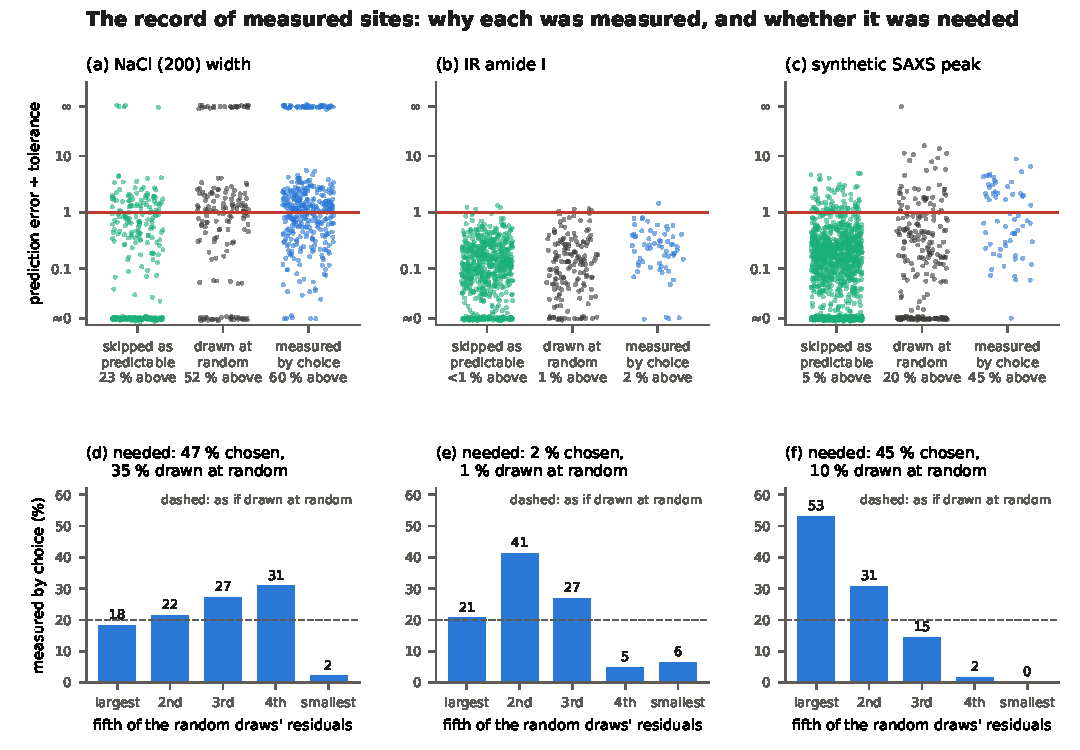
\includegraphics[width=\textwidth,height=0.44\textheight,keepaspectratio]{figures/figS8_measured}
\caption{The record of measured sites for one campaign of average cost per dataset. (a--c) Error of the frozen prediction divided by the tolerance (NaCl: width error ÷ 0.02 nm\ensuremath{^{-1}}; synthetic map: mean over the profile of the intensity error ÷ (0.005 \ensuremath{\times} intensity + 0.005); IR map: mean over channels of the absorbance error ÷ (0.10 \ensuremath{\times} absorbance + 0.10)) at every site of the guaranteed levels, grouped by action: skipped as predictable only, skipped under both claims (wrong only where the line is also of interest), measured as a random calibration draw, measured by choice. Red: one, a miss by exactly the tolerance; above it the prediction fails; \ensuremath{\approx}0: agreed absence or a residual below 0.013; \ensuremath{\infty}: presence predicted wrongly. Percentages give the share above the tolerance over 250 campaigns. (d--f) Residuals of the sites measured by choice, ranked among the calibration residuals of their level (randomised conformal p-value, SI 8 text): share falling in each fifth of the calibration residuals, from the largest to the smallest. Dashed: 20 \%, expected if measuring by choice were no better than drawing at random. Titles give the share of sites needed among those measured by choice and among those drawn at random, over 250 campaigns.}\label{fig:S8}
\end{figure}

\hypertarget{si-9.-the-map-bound}{%
\section*{SI 9. The map bound}\label{si-9.-the-map-bound}}
\addcontentsline{toc}{section}{SI 9. The map bound}

The calibration draw of a level serves a second purpose. Its interpolation labels are the errors, at the sites of the new level, of the map built from all coarser measurements. They therefore measure how well that map predicts at the density of the new level.

Let level \(L + 1\) have \(N\) sites, of which \(K\) lie outside tolerance of the map frozen before its draw. The \(m\) calibration sites are a uniform sample without replacement, so the number \(f\) of failures among them is hypergeometric. The map bound is the exact upper limit for a draw without replacement: the largest share \(K'/N\) for which the observed \(f\) is not rejected at level \(\delta_{\mathrm{map}}\),

\[
u(f) = \max \{ K'/N : P(H_{N, K', m} \le f) > \delta_{\mathrm{map}} \}
\]

with \(H_{N, K', m}\) hypergeometric, \(N\) sites of which \(K'\) fail and \(m\) draws. It holds with probability at least \(1 - \delta_{\mathrm{map}}\) for every \(K\), by the same inversion of the tail as Proposition A.1. The record also stores the Clopper--Pearson limit \cite{ClopperPearson1934}, \(\mathrm{Beta}^{-1}(1 - \delta_{\mathrm{map}};\ f + 1,\ m - f)\), which is exact for a binomial count, wider at the sizes of this study, and can fall short by a few per cent when the failing share is close to one.

\textbf{Sharing the draw with the decision.} The same draw sets the thresholds of level \(L + 1\). The decision fails with probability at most \(\delta_{L+1}\) and the map bound with probability at most \(\delta_{\mathrm{map}}\), so by the union bound both hold together with probability at least

\[
1 - \delta_{L+1} - \delta_{\mathrm{map}}
\]

No independence between the two statements is needed.

\textbf{Sites of interest.} Given the number \(m_Z\) of calibration sites of interest, those sites are a uniform sample without replacement from the sites of interest of the level. The same limit, applied to their failures, bounds the failing share among the sites of interest. This is the label-conditional statement of Section 3.4, at the cost of a smaller sample.

\textbf{Scope.} The bound concerns the map frozen before the draw, at the sites of the new level. The final map also uses the calibration sites and every site measured because no claim covered it. Those depend on the draw, so the plan gives the final map no finite-sample statement; the audit of Section 3.6 gives it one, and here it is also checked against the truth (Section 5.4).

\textbf{Record.} The map bound states, from the calibration draw of a level, how many of its sites the map built from coarser levels predicts outside tolerance. Recomputed with the exact limit from the 250 campaigns of each main configuration, it held on 95.8 \% of the guaranteed levels for IR, 84.4 \% for NaCl and 87.2 \% for the synthetic map, against confidences of 0.75, 0.80 and 0.80; the Clopper--Pearson limit held on 100 \%, 88.5 \% and 90.9 \%, at mean upper limits 0.052, 0.593 and 0.483 against 0.042, 0.579 and 0.463 for the exact one. On NaCl about half of the last-level sites lie outside that tolerance; the skip guarantee concerns only the sites a claim covers.

\hypertarget{si-10.-checks-beyond-the-level}{%
\section*{SI 10. Checks beyond the level}\label{si-10.-checks-beyond-the-level}}
\addcontentsline{toc}{section}{SI 10. Checks beyond the level}

The studies below extend the run record of SI 5 in four directions: a bound on the sites of interest lost, drift during a campaign, an audit of the finished map, and the cost of a specification against its calibration size and confidence. Every study uses the matched-quantile rule with natural-neighbour interpolation and the budgets of Table 3 unless stated otherwise.

\hypertarget{si-10.1-a-label-conditional-bound-for-the-sites-of-interest}{%
\subsection*{SI 10.1 A label-conditional bound for the sites of interest}\label{si-10.1-a-label-conditional-bound-for-the-sites-of-interest}}
\addcontentsline{toc}{subsection}{SI 10.1 A label-conditional bound for the sites of interest}

\textbf{Rule.} The study uses the two-claim variant of the synthetic map (SI 6.2), where a third of the sites are of interest. On each level the shared budget is kept at 0.20 with confidence 0.80. In addition, the share of the level\textquotesingle s sites of interest skipped under the no-interest claim is bounded by 0.20 with confidence 0.80. Given their number \(m_Z\), the calibration sites of interest are a uniform sample without replacement from the \(N_Z\) sites of interest of the level. \(N_Z\) is unknown, but it lies between \(m_Z\) and \(N_L - (m - m_Z)\). The allowed number \(k_Z\) of calibration sites of interest that the no-interest claim may cover is the largest \(k\) for which

\[
\max_{N_Z} P\big(H_{N_Z,\ \lfloor 0.20 N_Z \rfloor + 1,\ m_Z} \le k\big) \le 0.20
\]

and the no-interest claim covers only sites whose entry time on the path lies below the \((k_Z + 1)\)-th smallest entry time among the calibration sites of interest. With 12 to 20 such sites per level, \(k_Z\) was 0, 1 or 2. Restricting the cover of one claim keeps the shared-event bound, which holds for any subset of the cover it guarantees.

\textbf{Result.} Over 250 campaigns (Table S10.1), the plan lost 8.5 \ensuremath{\pm} 4.4 \% of the sites of interest on guaranteed levels under the no-interest claim, against 34.7 \ensuremath{\pm} 8.5 \% without the conditional bound, and measured 359 \ensuremath{\pm} 26 sites against 334 \ensuremath{\pm} 26. Of 1500 level checks, 4.9 \% exceeded the share of 0.20 that the conditional bound allows to fail at 20 \%; without the conditional bound, 58.7 \% did. The shared budget was exceeded on 2 of 1500 level checks, against 11.3 \% expected under the picked failure probabilities: the restricted cover leaves the shared rate well below its budget.

On the NaCl scan, where about two thirds of the sites hold the line, the same rule over 250 campaigns lost 8.1 \ensuremath{\pm} 3.0 \% of the sites of interest, against 9.2 \ensuremath{\pm} 3.2 \% without it, at 630 \ensuremath{\pm} 59 measurements against 614 \ensuremath{\pm} 56; 1.4 \% of level checks exceeded the share, against 2.2 \% without the statement. Where signal is common, the shared budget already spares it, and the conditional bound changes little and costs little.

{\renewcommand{\thetable}{S10.1}\small
\begin{longtable}[]{@{}
  >{\raggedright\arraybackslash}p{(\columnwidth - 12\tabcolsep) * \real{0.1429}}
  >{\raggedright\arraybackslash}p{(\columnwidth - 12\tabcolsep) * \real{0.1429}}
  >{\raggedright\arraybackslash}p{(\columnwidth - 12\tabcolsep) * \real{0.1429}}
  >{\raggedright\arraybackslash}p{(\columnwidth - 12\tabcolsep) * \real{0.1429}}
  >{\raggedright\arraybackslash}p{(\columnwidth - 12\tabcolsep) * \real{0.1429}}
  >{\raggedright\arraybackslash}p{(\columnwidth - 12\tabcolsep) * \real{0.1429}}
  >{\raggedright\arraybackslash}p{(\columnwidth - 12\tabcolsep) * \real{0.1429}}@{}}
\caption{Sites of interest lost under the no-interest claim on the two-claim variant of the synthetic map, per guaranteed level (mean over 250 campaigns).}\label{tab:S10.1}\\

\toprule\noalign{}
\begin{minipage}[b]{\linewidth}\raggedright
Level
\end{minipage} & \begin{minipage}[b]{\linewidth}\raggedright
3
\end{minipage} & \begin{minipage}[b]{\linewidth}\raggedright
4
\end{minipage} & \begin{minipage}[b]{\linewidth}\raggedright
5
\end{minipage} & \begin{minipage}[b]{\linewidth}\raggedright
6
\end{minipage} & \begin{minipage}[b]{\linewidth}\raggedright
7
\end{minipage} & \begin{minipage}[b]{\linewidth}\raggedright
8
\end{minipage} \\
\midrule\noalign{}
\endhead
\bottomrule\noalign{}
\endlastfoot
Shared budget only & 0.0 \% & 12.0 \% & 25.1 \% & 32.6 \% & 35.4 \% & 38.9 \% \\
With the label-conditional bound & 0.0 \% & 5.0 \% & 6.8 \% & 7.6 \% & 9.3 \% & 9.1 \% \\
\end{longtable}
}

\hypertarget{si-10.2-drift-during-a-campaign}{%
\subsection*{SI 10.2 Drift during a campaign}\label{si-10.2-drift-during-a-campaign}}
\addcontentsline{toc}{subsection}{SI 10.2 Drift during a campaign}

\textbf{Model.} The synthetic sample swells slowly while it is measured: a measurement at clock \(t\), the number of sites measured before it, returns the profile of the sample as it was when the plan was declared, with \(q\) scaled by \(1 + s\,t/932\), so that every feature moves to lower \(q\). Here 932 is the mean cost of the plan in the record, and \(s\) takes the values 0, 0.05, 0.10 and 0.20. Claim and budget are those of the main text: the full profile within 0.5 \% + 0.005 on average, \(R_E \le 0.10\) at confidence 0.80 per level. Calibration labels compare the prediction with the drifted measurement, as a live campaign would; every rate is counted against the sample at the start. After each level, five seed sites fixed in advance are measured again and compared, under the claim\textquotesingle s metric, with their first measurement; a failure flags the level. Re-measurement is not charged to the clock. At \(s = 0\) the campaigns reproduce the record site for site. Fifty campaigns were run per value.

\textbf{Result.} Under the profile claim the bound broke (Table S10.2). At \(s = 0.05\) and \(0.10\) the levels exceeded their budget in 24 \% of checks, against 9.5 \% expected under the picked failure probabilities, although drifted calibration sites disagree with earlier predictions and the rule skipped less: the plan measured 1687 \ensuremath{\pm} 76 and 1806 \ensuremath{\pm} 51 sites against 966 \ensuremath{\pm} 247 without drift. At \(s = 0.20\) it measured almost every site, and the few skips met the budget. Most of the damage lay in the measured sites: 88 \% to 96 \% of the sites measured on guaranteed levels returned a profile outside tolerance of the sample at the start, and those sites carry no claim. The repeated seed sites flagged no level without drift and flagged every drifted campaign, from the fourth level on at \(s = 0.05\) and from the third at the larger values. The synthetic profiles carry no noise, so any failure of a repeated site signals drift; with noise, the threshold for a flag comes from repeated measurements, as for the NaCl scan in SI 2. The two-claim variant of the synthetic map (SI 6.2), with its peak-position tolerance of 0.005 \AA{}\ensuremath{^{-1}}, absorbed a stretch of 5 \% and kept its bound at every stretch, while 21 \% to 79 \% of its measurements went outside tolerance at stretches of 10 \% and 20 \%; the archive of SI 5 keeps those runs.

{\renewcommand{\thetable}{S10.2}\small
\begin{longtable}[]{@{}
  >{\raggedright\arraybackslash}p{(\columnwidth - 8\tabcolsep) * \real{0.2000}}
  >{\raggedright\arraybackslash}p{(\columnwidth - 8\tabcolsep) * \real{0.2000}}
  >{\raggedright\arraybackslash}p{(\columnwidth - 8\tabcolsep) * \real{0.2000}}
  >{\raggedright\arraybackslash}p{(\columnwidth - 8\tabcolsep) * \real{0.2000}}
  >{\raggedright\arraybackslash}p{(\columnwidth - 8\tabcolsep) * \real{0.2000}}@{}}
\caption{Drift on the synthetic map, 50 campaigns per value of \(s\). Level checks over budget, against 9.5 \% expected under the picked failure probabilities; measured sites outside tolerance of the sample at the start, as a share of the measured sites of guaranteed levels; campaigns with at least one flagged level.}\label{tab:S10.2}\\

\toprule\noalign{}
\begin{minipage}[b]{\linewidth}\raggedright
\(s\)
\end{minipage} & \begin{minipage}[b]{\linewidth}\raggedright
Sites measured
\end{minipage} & \begin{minipage}[b]{\linewidth}\raggedright
Level checks over budget
\end{minipage} & \begin{minipage}[b]{\linewidth}\raggedright
Measured sites off the sample
\end{minipage} & \begin{minipage}[b]{\linewidth}\raggedright
Campaigns flagged
\end{minipage} \\
\midrule\noalign{}
\endhead
\bottomrule\noalign{}
\endlastfoot
0.00 & 966 \ensuremath{\pm} 247 & 9.7 \% & 0 \% & 0 \% \\
0.05 & 1687 \ensuremath{\pm} 76 & 23.7 \% & 88 \% & 100 \% \\
0.10 & 1806 \ensuremath{\pm} 51 & 23.7 \% & 93 \% & 100 \% \\
0.20 & 1908 \ensuremath{\pm} 45 & 4.0 \% & 96 \% & 100 \% \\
\end{longtable}
}

\textbf{Correction.} A drift detected in this way can be modelled from the repeated sites and removed from the measurements, or the calibration sites can be weighted by their age, which keeps a bound with a coverage loss that grows with the shift \cite{Barber2023}; when the shift is known, as for covariate shift, likelihood-ratio weights restore exact coverage \cite{Tibshirani2019}. Neither was simulated here.

\hypertarget{si-10.3-the-audit-of-the-finished-map}{%
\subsection*{SI 10.3 The audit of the finished map}\label{si-10.3-the-audit-of-the-finished-map}}
\addcontentsline{toc}{subsection}{SI 10.3 The audit of the finished map}

\textbf{Protocol.} After the last level, \(n_a\) sites are drawn uniformly without replacement from the skipped sites of the guaranteed levels, measured and kept out of the map. The map predicts every skipped site from all other measured sites with the protocol\textquotesingle s predictor, as for the final maps of SI 5.3. With \(N\) skipped sites, of which \(K\) lie outside tolerance, and \(f\) failing audit sites, the bound on \(K\) is the exact hypergeometric limit of SI 9,

\[
u(f) = \max \{ K' : P(H_{N, K', n_a} \le f) > 1 - c \}
\]

reported as a share \(u(f)/N_c\) of the \(N_c\) sites of the guaranteed levels. Coverage was estimated over the 250 campaigns of the record, with 200 audit draws per campaign on the IR and NaCl maps and 50 on the synthetic map. On the two-claim variant of the synthetic map the audit was also stratified by the claim of the skip, 50 sites under the no-interest claim and 50 under the interpolation claim alone, each stratum bounded at \(1 - (1 - c)/2\) and the bounds summed. Within the no-interest stratum, a separate draw of 100 audit sites, beyond the 50 + 50 of the stratified audit and with its own confidence, bounds the number \(K_Z\) of sites of interest skipped there; with \(M_Z\) sites of interest measured on guaranteed levels, the share of the sites of interest lost is at most \(u_Z/(M_Z + u_Z)\), because that share grows with \(K_Z\) and the sites of interest number at least \(M_Z + K_Z\).

{\renewcommand{\thetable}{S10.3}\small
\begin{longtable}[]{@{}
  >{\raggedright\arraybackslash}p{(\columnwidth - 12\tabcolsep) * \real{0.1429}}
  >{\raggedright\arraybackslash}p{(\columnwidth - 12\tabcolsep) * \real{0.1429}}
  >{\raggedright\arraybackslash}p{(\columnwidth - 12\tabcolsep) * \real{0.1429}}
  >{\raggedright\arraybackslash}p{(\columnwidth - 12\tabcolsep) * \real{0.1429}}
  >{\raggedright\arraybackslash}p{(\columnwidth - 12\tabcolsep) * \real{0.1429}}
  >{\raggedright\arraybackslash}p{(\columnwidth - 12\tabcolsep) * \real{0.1429}}
  >{\raggedright\arraybackslash}p{(\columnwidth - 12\tabcolsep) * \real{0.1429}}@{}}
\caption{Audit of the final maps of the record: true share of sites on guaranteed levels the final map predicts outside tolerance (mean over 250 campaigns), mean audit bound and coverage over the audit draws (250 \ensuremath{\times} 200; synthetic 250 \ensuremath{\times} 50).}\label{tab:S10.3}\\

\toprule\noalign{}
\begin{minipage}[b]{\linewidth}\raggedright
Map
\end{minipage} & \begin{minipage}[b]{\linewidth}\raggedright
True share
\end{minipage} & \begin{minipage}[b]{\linewidth}\raggedright
\(n_a\)
\end{minipage} & \begin{minipage}[b]{\linewidth}\raggedright
Bound at 0.80
\end{minipage} & \begin{minipage}[b]{\linewidth}\raggedright
Coverage at 0.80
\end{minipage} & \begin{minipage}[b]{\linewidth}\raggedright
Bound at 0.95
\end{minipage} & \begin{minipage}[b]{\linewidth}\raggedright
Coverage at 0.95
\end{minipage} \\
\midrule\noalign{}
\endhead
\bottomrule\noalign{}
\endlastfoot
IR map & 0.4 \% & 50 & 2.7 \% & 100.0 \% & 4.8 \% & 100.0 \% \\
& & 100 & 1.5 \% & 100.0 \% & 2.6 \% & 100.0 \% \\
& & 200 & 0.9 \% & 95.5 \% & 1.5 \% & 100.0 \% \\
NaCl scan & 18.0 \% & 50 & 20.9 \% & 84.1 \% & 23.4 \% & 96.4 \% \\
& & 100 & 19.8 \% & 83.0 \% & 21.5 \% & 96.1 \% \\
& & 200 & 19.0 \% & 82.5 \% & 20.0 \% & 96.0 \% \\
Synthetic map & 3.6 \% & 50 & 6.2 \% & 89.2 \% & 8.4 \% & 98.8 \% \\
& & 100 & 5.1 \% & 86.2 \% & 6.5 \% & 97.3 \% \\
& & 200 & 4.5 \% & 84.6 \% & 5.4 \% & 96.6 \% \\
\end{longtable}
}

On the two-claim variant of the synthetic map (SI 6.2), the stratified audit of 100 sites bounded the share at 14.6 \% at 0.80 (coverage 96.1 \%) and 17.8 \% at 0.95 (coverage 99.5 \%). From 100 sites of the no-interest stratum, the share of the sites of interest lost under the no-interest claim, 34.7 \% on average, was bounded at 66.6 \% at 0.80 (coverage 100.0 \%) and 69.9 \% at 0.95 (coverage 100.0 \%), a statement that needs no change to the campaign but is loose: the measured sites of interest are few, and the label-conditional rule of SI 10.1 bounds the same share at 0.20. Stratification cost more than it gained here, because each stratum carries half the confidence.

\textbf{A Gaussian-process acquisition campaign.} On the NaCl scan a campaign was steered by the process of SI 7: presence and log width each modelled by a Gaussian process with RBF and white-noise kernel, maximum likelihood, from the seed sites on. In batches of 25, it measured the unmeasured sites with the largest posterior probability that skipping them would be wrong, the probability being the presence probability for a predicted absent line and one minus the probability of presence within tolerance otherwise (SI 7), with the predictive standard deviation. At 614, 694 and 800 sites measured, the map predicted every other site, and 100 audit sites drawn uniformly from the unmeasured sites bounded its errors at confidence 0.80; the campaign is deterministic, so coverage is over 2000 audit draws (Table S10.4).

{\renewcommand{\thetable}{S10.4}\small
\begin{longtable}[]{@{}
  >{\raggedright\arraybackslash}p{(\columnwidth - 10\tabcolsep) * \real{0.1667}}
  >{\raggedright\arraybackslash}p{(\columnwidth - 10\tabcolsep) * \real{0.1667}}
  >{\raggedright\arraybackslash}p{(\columnwidth - 10\tabcolsep) * \real{0.1667}}
  >{\raggedright\arraybackslash}p{(\columnwidth - 10\tabcolsep) * \real{0.1667}}
  >{\raggedright\arraybackslash}p{(\columnwidth - 10\tabcolsep) * \real{0.1667}}
  >{\raggedright\arraybackslash}p{(\columnwidth - 10\tabcolsep) * \real{0.1667}}@{}}
\caption{Gaussian-process acquisition campaign on the NaCl scan: share of the 995 sites on guaranteed levels the map gets wrong, the process\textquotesingle s own stated share with predictive and latent standard deviation, and the audit bound from 100 sites at confidence 0.80 (mean, 10 \% and 90 \% quantiles over 2000 draws, coverage).}\label{tab:S10.4}\\

\toprule\noalign{}
\begin{minipage}[b]{\linewidth}\raggedright
Sites measured
\end{minipage} & \begin{minipage}[b]{\linewidth}\raggedright
True share
\end{minipage} & \begin{minipage}[b]{\linewidth}\raggedright
Stated, predictive
\end{minipage} & \begin{minipage}[b]{\linewidth}\raggedright
Stated, latent
\end{minipage} & \begin{minipage}[b]{\linewidth}\raggedright
Audit bound (10--90 \%)
\end{minipage} & \begin{minipage}[b]{\linewidth}\raggedright
Coverage
\end{minipage} \\
\midrule\noalign{}
\endhead
\bottomrule\noalign{}
\endlastfoot
614 & 9.0 \% & 11.2 \% & 3.9 \% & 10.6 \% (8.4--12.8 \%) & 80.5 \% \\
694 & 6.1 \% & 7.2 \% & 3.3 \% & 7.3 \% (5.6--8.8 \%) & 80.2 \% \\
800 & 1.6 \% & 2.2 \% & 2.1 \% & 2.2 \% (1.6--2.8 \%) & 91.0 \% \\
\end{longtable}
}

At the cost of the guaranteed plan, the acquisition campaign left fewer wrong sites than the guaranteed plan\textquotesingle s final map, 9.0 \% against 18.0 \%, with a different predictor and no stated bound. Its own statement held with the predictive standard deviation and was 2.3 times too low with the latent one, and nothing within the campaign told the two apart; the audit did, at a cost of 100 measurements.

\textbf{A Gaussian-process campaign told to meet a budget.} The same campaign was run 30 times with a stopping rule: after every batch the process stated its share of sites on guaranteed levels predicted wrongly, the sum of its per-site probabilities of a skip error, and stopped once the statement reached 0.20. Each batch was chosen among a random 80 \% of the unmeasured sites, so runs differ; acquisition used the predictive probability, and the stopping point of the latent rule was read off the same trajectories. With the predictive standard deviation the runs stopped after 451 to 501 measurements (mean 467) at 14.6 \ensuremath{\pm} 0.6 \%, all within the budget. An audit of 100 unmeasured sites at confidence 0.80, taken at the stopping point, bounded the share at or below 0.20 in 89 \% of draws. With the latent standard deviation, which leaves out the noise of a single measurement, the statement was 11.6 \% before any site beyond the seed was measured, so every run would have stopped at the 76 seed sites, with 36.8 \% of the sites on guaranteed levels predicted wrongly. For comparison, the plans guaranteed level by level measured 614 \ensuremath{\pm} 56 sites; their skip errors, the quantity they bound, exceeded 20 \% of the sites on guaranteed levels in 1.2 \% of campaigns, and their final maps, which carry no statement, in 30 \%.

\hypertarget{si-10.4-cost-against-calibration-size-and-confidence}{%
\subsection*{SI 10.4 Cost against calibration size and confidence}\label{si-10.4-cost-against-calibration-size-and-confidence}}
\addcontentsline{toc}{subsection}{SI 10.4 Cost against calibration size and confidence}

{\renewcommand{\thetable}{S10.5}\small
\begin{longtable}[]{@{}
  >{\raggedright\arraybackslash}p{(\columnwidth - 10\tabcolsep) * \real{0.1667}}
  >{\raggedright\arraybackslash}p{(\columnwidth - 10\tabcolsep) * \real{0.1667}}
  >{\raggedright\arraybackslash}p{(\columnwidth - 10\tabcolsep) * \real{0.1667}}
  >{\raggedright\arraybackslash}p{(\columnwidth - 10\tabcolsep) * \real{0.1667}}
  >{\raggedright\arraybackslash}p{(\columnwidth - 10\tabcolsep) * \real{0.1667}}
  >{\raggedright\arraybackslash}p{(\columnwidth - 10\tabcolsep) * \real{0.1667}}@{}}
\caption{Plans guaranteed level by level on the IR map at \(\varepsilon = 0.10\), 100 campaigns per setting: allowed numbers \(k\) of failing calibration sites, sites measured of 959, and level checks over budget against the share expected under the picked failure probabilities.}\label{tab:S10.5}\\

\toprule\noalign{}
\begin{minipage}[b]{\linewidth}\raggedright
\(m\)
\end{minipage} & \begin{minipage}[b]{\linewidth}\raggedright
Confidence
\end{minipage} & \begin{minipage}[b]{\linewidth}\raggedright
\(k\)
\end{minipage} & \begin{minipage}[b]{\linewidth}\raggedright
Sites measured
\end{minipage} & \begin{minipage}[b]{\linewidth}\raggedright
Level checks over budget
\end{minipage} & \begin{minipage}[b]{\linewidth}\raggedright
Expected
\end{minipage} \\
\midrule\noalign{}
\endhead
\bottomrule\noalign{}
\endlastfoot
20 & 0.80 & 0 & 340 \ensuremath{\pm} 90 & 0.8 \% & 9.2 \% \\
20 & 0.90 & none, 0 & 851 \ensuremath{\pm} 30 & 0.8 \% & 3.7 \% \\
20 & 0.95 & none & 959 \ensuremath{\pm} 0 & 0.0 \% & 0.0 \% \\
40 & 0.80 & 1, 2 & 337 \ensuremath{\pm} 63 & 0.5 \% & 11.7 \% \\
40 & 0.90 & 1, 2 & 359 \ensuremath{\pm} 65 & 0.5 \% & 5.8 \% \\
40 & 0.95 & 0, 1 & 430 \ensuremath{\pm} 78 & 0.0 \% & 1.8 \% \\
80 & 0.80 & 5, 6, 7 & 393 \ensuremath{\pm} 22 & 0.0 \% & 10.0 \% \\
80 & 0.90 & 4, 5, 7 & 408 \ensuremath{\pm} 36 & 0.0 \% & 4.1 \% \\
80 & 0.95 & 3, 4, 7 & 436 \ensuremath{\pm} 46 & 0.0 \% & 2.1 \% \\
\end{longtable}
}

At \(m = 20\) the smallest budget the draw can support, \(1 - \delta^{1/m}\) in the binomial approximation, is 0.08 at confidence 0.80 and exceeds 0.10 at 0.90 and 0.95, so most levels at 0.90 and all at 0.95 have no threshold ("none") and are measured in full. At \(m = 80\) every threshold exists, and the calibration sample itself, 320 sites over four guaranteed levels, sets most of the cost on a map of 959 sites. On the IR map few calibration failures occur, so the exceedances lie far below the expected share at every setting.


\IfFileExists{iopart-num.bst}{\bibliographystyle{iopart-num}}{\bibliographystyle{unsrt}}
\bibliography{refs}

\end{document}
